%%%%%%%%%%%%%%%%%%%%%%%%%%%%%%%%%%%%%%%%%
% Masters/Doctoral Thesis
% LaTeX Template
% Version 2.5 (27/8/17)
%
% This template was downloaded from:
% http://www.LaTeXTemplates.com
%
% Version 2.x major modifications by:
% Vel (vel@latextemplates.com)
%
% This template is based on a template by:
% Steve Gunn (http://users.ecs.soton.ac.uk/srg/softwaretools/document/templates/)
% Sunil Patel (http://www.sunilpatel.co.uk/thesis-template/)
%
% Template license:
% CC BY-NC-SA 3.0 (http://creativecommons.org/licenses/by-nc-sa/3.0/)
%
%%%%%%%%%%%%%%%%%%%%%%%%%%%%%%%%%%%%%%%%%

%----------------------------------------------------------------------------------------
%  PACKAGES AND OTHER DOCUMENT CONFIGURATIONS
%----------------------------------------------------------------------------------------
\documentclass[11pt, oneside, english, singlespacing, headsepline]{MastersDoctoralThesis}

% --- Load all packages and configurations from your preamble file ---
%%%%%%%%%%%%%%%%%%%%%%%%%%%%%%%%%%%%%%%%%
% PREAMBLE & CONFIGURATION
%%%%%%%%%%%%%%%%%%%%%%%%%%%%%%%%%%%%%%%%%

%----------------------------------------------------------------------------------------
%   PACKAGES
%----------------------------------------------------------------------------------------
\usepackage[utf8]{inputenc} % Required for inputting international characters
\usepackage[T1]{fontenc} % Output font encoding for international characters
\usepackage{lmodern} % Scalable T1 font required for microtype expansion on this system
\usepackage[final]{microtype} % Better kerning, font expansion, and protrusion to mitigate small overfull boxes
\microtypesetup{protrusion=true, expansion=true}
\usepackage{amsmath} % Required for advanced math environments like equation*
\usepackage{amssymb} % Required for \mathbb and \checkmark
\usepackage[backend=biber, sorting=none, natbib=true]{biblatex}\usepackage[autostyle=true]{csquotes} % Required for language-dependent quotes
\usepackage{graphicx} % Required for images

% Shrink a math block to fit \linewidth only when it is too wide (never enlarge).
\newsavebox{\iseqlbox}
\newcommand{\iseqlfit}[1]{%
  \sbox{\iseqlbox}{#1}%
  \ifdim\wd\iseqlbox>\linewidth
    \resizebox{\linewidth}{!}{\usebox{\iseqlbox}}%
  \else
    \usebox{\iseqlbox}%
  \fi}

% --- TikZ for ISEQL interval diagrams
\usepackage{tikz}
\usetikzlibrary{arrows,shapes,arrows.meta,calc,math,positioning}

\tikzstyle{interval}            = [line width = 1pt, > = {Circle[length = 3.4pt]}, shorten > = -0pt]
\tikzstyle{interval label}      = [font = {\small}]

\newcommand*{\Interval}[5][]{%
    \draw[interval, #1] (#2, #4) -- (#3, #4);
    \node[interval label] at (-0.5,#4) {#5};
}

\newcommand*{\RSIntervals}[6]{%
    \Interval[#1]{#2}{#3}{1}{$r$}
    \Interval[#4]{#5}{#6}{0}{$s$}
}

\newcommand*{\DoodleSP}{%
    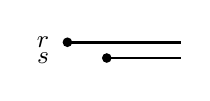
\begin{tikzpicture}[xscale=0.5, yscale=0.2, baseline={($(current bounding box.north)-(0,7.5pt)$)}]
        \RSIntervals{<-}{0}{3}{<-}{1}{3}
    \end{tikzpicture}%
}

\newcommand*{\DoodleBef}{%
    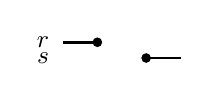
\begin{tikzpicture}[xscale=0.5, yscale=0.2, baseline={($(current bounding box.north)-(0,7.5pt)$)}]
        \RSIntervals{->}{0}{1}{<-}{2}{3}
    \end{tikzpicture}%
}

\newcommand*{\DoodleLOJ}{%
    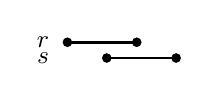
\begin{tikzpicture}[xscale=0.5, yscale=0.2, baseline={($(current bounding box.north)-(0,7.5pt)$)}]
        \RSIntervals{<->}{0}{2}{<->}{1}{3}
    \end{tikzpicture}%
}

\newcommand*{\DoodleDJ}{%
    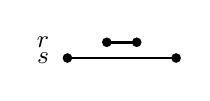
\begin{tikzpicture}[xscale=0.5, yscale=0.2, baseline={($(current bounding box.north)-(0,7.5pt)$)}]
        \RSIntervals{<->}{1}{2}{<->}{0}{3}
    \end{tikzpicture}%
}

\newcommand*{\DoodleEF}{%
    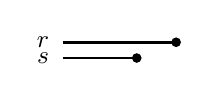
\begin{tikzpicture}[xscale=0.5, yscale=0.2, baseline={($(current bounding box.north)-(0,7.5pt)$)}]
        \RSIntervals{->}{0}{3}{->}{0}{2}
    \end{tikzpicture}%
}

% --- ISEQL temporal operators
\newcommand*{\Bef}{\mathrm{Bef}}
\newcommand*{\SP}{\mathrm{SP}}
\newcommand*{\LOJ}{\mathrm{LOJ}}
\newcommand*{\DJoin}{\mathrm{DJ}}
\newcommand*{\EF}{\mathrm{EF}}
\usepackage{siunitx} % Required for SI units
\usepackage{xurl} % Allow better URL line breaks (especially in bibliography)
\emergencystretch=2em % Relax line-breaking slightly to avoid overfull \hbox warnings
\usepackage{booktabs} % For professional-looking tables
\usepackage{pifont} % Required for \ding symbols
\newcommand{\xmark}{\text{\ding{55}}} % Cross mark symbol
\usepackage{tabularx} % For tables with automatic line wrapping
\usepackage{longtable} % For tables that span multiple pages
\usepackage{caption}  % For table captions
\usepackage{listings}
\lstset{
  basicstyle=\small\ttfamily,
  breaklines=true,
  breakatwhitespace=true,
  columns=fullflexible,
  frame=single,
  xleftmargin=2em,
  framexleftmargin=1em
}

%----------------------------------------------------------------------------------------
%   BIBLIOGRAPHY
%----------------------------------------------------------------------------------------
\addbibresource{references.bib} % The filename of the bibliography
% Improve URL line breaking in bibliography entries
\Urlmuskip=0mu plus 1mu\relax
\setcounter{biburlnumpenalty}{100}
\setcounter{biburlucpenalty}{100}
\setcounter{biburllcpenalty}{100}

%----------------------------------------------------------------------------------------
%   MARGIN SETTINGS
%----------------------------------------------------------------------------------------
\geometry{
  paper=a4paper, % Change to letterpaper for US letter
  inner=2.5cm, % Inner margin
  outer=3.8cm, % Outer margin
  bindingoffset=.5cm, % Binding offset
  top=1.5cm, % Top margin
  bottom=1.5cm, % Bottom margin
}
%----------------------------------------------------------------------------------------
%   THESIS INFORMATION
%----------------------------------------------------------------------------------------
% Update these values before you start writing.
\newcommand{\thesistypename}{Master Thesis}
\newcommand{\programmename}{Joint Degree of Master of Science in Mathematical Modelling in Engineering: Theory, Numerics, Applications}
\newcommand{\academicyear}{2026--2027}
\newcommand{\titlepagelogo}{Figures/Logos/univaq.png}
\newcommand{\titlepagepartnerlogo}{Figures/Logos/uhh.jpg}
\newcommand{\programmelogo}{Figures/Logos/mathmods.jpg}
\newcommand{\titlepagelogosize}{2.7cm}
\newcommand{\titlepagelogowidth}{4.8cm}
\newcommand{\titlepagelogoleftlabel}{UNIVERSIT\`A DEGLI STUDI DELL'AQUILA}
\newcommand{\titlepagelogorightlabel}{UNIVERSIT\"AT HAMBURG}
\newcommand{\titlepagelogolefturl}{https://www.univaq.it/en/}
\newcommand{\titlepagelogorighturl}{https://www.uni-hamburg.de/}
\newcommand{\programmeurl}{https://www.mathmods.eu/}
\newcommand{\authorurl}{https://github.com/ghiffaryr}
\newcommand{\supervisorurl}{https://www.disim.univaq.it/FabioPersia}
\newcommand{\departmenturl}{https://www.disim.univaq.it/}

\newcommand{\printtitlepagelogos}{%
  \begingroup
  \setlength{\tabcolsep}{12pt}%
  \begin{tabular}{@{}cc@{}}
    \parbox[c]{\titlepagelogowidth}{\centering
      \parbox[c][\titlepagelogosize][c]{\titlepagelogosize}{\centering\includegraphics[width=\titlepagelogosize,height=\titlepagelogosize,keepaspectratio]{\titlepagelogo}}\\[0.3cm]
      \href{\titlepagelogolefturl}{\titlepagelogoleftlabel}
    } &
    \parbox[c]{\titlepagelogowidth}{\centering
      \parbox[c][\titlepagelogosize][c]{\titlepagelogosize}{\centering\includegraphics[width=\titlepagelogosize,height=\titlepagelogosize,keepaspectratio]{\titlepagepartnerlogo}}\\[0.3cm]
      \href{\titlepagelogorighturl}{\titlepagelogorightlabel}
    }
  \end{tabular}%
  \endgroup
}

\newcommand{\printprogrammelogo}{%
  \includegraphics[width=0.4\linewidth]{\programmelogo}%
}

\thesistitle{WATCHOUT ISEQL: Large Audio-Language Models and Object Re-Identification for Forensic Multimodal Surveillance Event Detection}
\supervisor{Prof. Fabio \textsc{Persia}}
\cosupervisor{}
\degree{Master of Science}
\author{Ghiffary \textsc{Rifqialdi}}
\subject{Computer Science}
\keywords{multimodal surveillance, forensic event detection, ISEQL, large audio-language models, object re-identification, vision-language models, three-condition ablation}

\university{UNIVERSIT\`A DEGLI STUDI DELL'AQUILA\\UNIVERSIT\"AT HAMBURG}
\department{\href{\departmenturl}{Department of Information Engineering, Information Sciences and Mathematics}}
\faculty{\href{http://faculty.university.com}{Faculty Name}}

%----------------------------------------------------------------------------------------
%   PDF METADATA
%----------------------------------------------------------------------------------------
\AtBeginDocument{
  \hypersetup{pdftitle=\ttitle} % Set the PDF's title to your title
  \hypersetup{pdfauthor=\authorname} % Set the PDF's author to your name
  \hypersetup{pdfkeywords=\keywordnames} % Set the PDF's keywords to your keywords
}

%----------------------------------------------------------------------------------------
%   CUSTOM PROGRAMME PAGE ENVIRONMENT
%----------------------------------------------------------------------------------------
\newenvironment{programmepage}{
  \thispagestyle{empty} % No page number
  \begin{center}
    % Use \vfill to create flexible vertical space
    \vspace*{0.01\textheight} % A smaller fixed space from the top
    \vfill % Fill the space above the text

    {\large\textbf{This thesis was conducted within \href{\programmeurl}{\programmename}.}}\par

    \vspace{4cm} % A fixed space between the text and the logo

    \printprogrammelogo

    \vfill % Fill the remaining space at the bottom of the page
  \end{center}
  \clearpage % Automatically starts a new page after this one
}{}
\usepackage{pdfpages}

% --- Document Body ---
\begin{document}

\frontmatter
\pagestyle{plain}

% --- TITLE PAGE ---
\includepdf{Chapters/CoverPage.pdf}

%----------------------------------------------------------------------------------------
%   PROGRAMME PAGE
%----------------------------------------------------------------------------------------
\begin{programmepage}
\end{programmepage}

%----------------------------------------------------------------------------------------
%  ABSTRACT
%----------------------------------------------------------------------------------------

\begin{abstract}
  \addchaptertocentry{\abstractname}

  This thesis presents WATCHOUT ISEQL, a forensic multimodal surveillance framework that combines visual perception from a vision-language model (VLM) with training-free object re-identification (prompt-based identity persistence over a memory of object embeddings, requiring no tracking model or fine-tuning) and environmental audio analysis from a large audio-language model (LALM), through a shared interval-based temporal representation. The study is organised as a three-condition ablation experiment: a visual-only condition (A) using a VLM with re-ID to extract frame-level relation triples, an audio-only condition (B) using either Qwen2-Audio-7B-Instruct (LALM) or PANNs CNN14, and a multimodal condition (C) that takes the UNION of A and B without temporal cross-modal joins.

  The evaluation on a novel 30-scene dataset generated with Dreamina Seedance across four VLM models and two audio providers demonstrates that condition C achieves at least the accuracy of the better unimodal condition on every scene. With the best combination (Gemini 3.6 Flash + Qwen2-Audio-7B), the system achieves 30/30 TP (F1 = 0.938, 4 FP, 0 FN). Object re-identification is essential for the tracking-dependent events (suspicious near vehicle, vehicle escape, handoff): without it, these duration-gated queries rarely fire, and re-ID lifts the best visual F1 from 0.622 to 0.885. The LALM (Qwen2-Audio-7B) achieves perfect precision (1.000) and outperforms PANNs CNN14 on audio-only detection (micro F1 = 0.788 vs 0.400). The UNION-based multimodal design preserves all detections from both modalities without the recall loss inherent in temporal cross-modal joins. Every event is the output of a SQL query, providing a fully auditable forensic pipeline.

  The implementation and the evaluation harness are available at \url{https://github.com/ghiffaryr/multimodal-surveillance-iseql}.
\end{abstract}

%----------------------------------------------------------------------------------------
%  ACKNOWLEDGEMENTS
%----------------------------------------------------------------------------------------
\begin{acknowledgements}
  \addchaptertocentry{\acknowledgementname}

  I would like to thank my supervisor, Prof. Fabio Persia, for his guidance.

  I extend my sincere thanks to the MathMods programme for fostering an international research experience. The research, implementation, and experiments presented in this thesis were carried out independently by me, using my own computational resources.

  Finally, I would like to thank my family for their unwavering support and encouragement throughout my studies.
\end{acknowledgements}

%----------------------------------------------------------------------------------------
%  LIST OF CONTENTS/FIGURES/TABLES PAGES
%----------------------------------------------------------------------------------------

\tableofcontents % Prints the main table of contents

\listoffigures % Prints the list of figures

\listoftables % Prints the list of tables

%----------------------------------------------------------------------------------------
%  ABBREVIATIONS
%----------------------------------------------------------------------------------------

\begin{abbreviations}{ll}
    \textbf{ISEQL} & Interval-based Surveillance Event Query Language \\
    \textbf{VLM} & Vision-Language Model \\
    \textbf{LALM} & Large Audio-Language Model \\
    \textbf{PANNs} & Pretrained Audio Neural Networks \\
    \textbf{ASR} & Automatic Speech Recognition \\
    \textbf{SER} & Speech Emotion Recognition \\
    \textbf{FP} & False Positive \\
    \textbf{FN} & False Negative \\
    \textbf{TP} & True Positive \\
    \textbf{TN} & True Negative \\
    \textbf{IoU} & Intersection over Union \\
    \textbf{mAP} & Mean Average Precision \\
    \textbf{CNN} & Convolutional Neural Network \\
    \textbf{SQL} & Structured Query Language \\
    \textbf{SQLite} & Structured Query Language Lite \\
    \textbf{REST} & Representational State Transfer \\
    \textbf{API} & Application Programming Interface \\
\end{abbreviations}

% %----------------------------------------------------------------------------------------
% %  PHYSICAL CONSTANTS/OTHER DEFINITIONS
% %----------------------------------------------------------------------------------------

% \begin{constants}{lr@{${}={}$}l} % The list of physical constants is a three column table

% % The \SI{}{} command is provided by the siunitx package, see its documentation for instructions on how to use it

% Speed of Light & $c_{0}$ & \SI{2.99792458e8}{\meter\per\second} (exact)\\
% %Constant Name & $Symbol$ & $Constant Value$ with units\\

% \end{constants}

% %----------------------------------------------------------------------------------------
% %  SYMBOLS
% %----------------------------------------------------------------------------------------

% \begin{symbols}{lll} % Include a list of Symbols (a three column table)

% $a$ & distance & \si{\meter} \\
% $P$ & power & \si{\watt} (\si{\joule\per\second}) \\
% %Symbol & Name & Unit \\

% \addlinespace % Gap to separate the Roman symbols from the Greek

% $\omega$ & angular frequency & \si{\radian} \\

% \end{symbols}

%----------------------------------------------------------------------------------------
%  DEDICATION
%----------------------------------------------------------------------------------------

\dedicatory{To my family, for their endless support and encouragement.}

%----------------------------------------------------------------------------------------
%  THESIS CONTENT - CHAPTERS
%----------------------------------------------------------------------------------------

\mainmatter % Begin numeric (1,2,3...) page numbering

\pagestyle{thesis} % Return the page headers back to the "thesis" style

% Include the chapters of the thesis as separate files from the Chapters folder
% Uncomment the lines as you write the chapters

\chapter{Introduction}
\label{Introduction}

Modern video surveillance systems generate continuous footage at a scale that far exceeds human monitoring capacity. A single security operator watching multiple camera feeds experiences \textit{vigilance decrement} ,  a well-documented decline in attention that sets in after approximately twenty minutes, causing a substantial fraction of visible events to go unnoticed. Automated systems aim to bridge this gap, but they face three persistent challenges. First, visual detectors must track objects across frames to form temporal intervals; without tracking, every frame assigns new identifiers and no interval spans long enough to constitute an event. Second, visual-only systems are blind to events outside the camera's field of view ,  a shout from an adjacent room, a vehicle collision behind a building. Third, naively fusing modalities through temporal alignment reduces recall, because a detection in one modality may fail to find a temporally coincident confirmation in the other.

This thesis addresses these challenges through \textbf{WATCHOUT ISEQL}, a multimodal forensic surveillance framework that combines visual perception from a vision-language model (VLM) with object re-identification and environmental sound analysis from a large audio-language model (LALM). The core of the system is ISEQL (Interval-based Surveillance Event Query Language) \citep{helmer2016highlevel}, which extends relational algebra with temporal operators derived from Allen's interval algebra \citep{allen1983}. The visual stream uses a VLM with a two-phase tracking prompt to maintain consistent object identities across frames, producing relation triples that are collapsed into time intervals. The audio stream uses either Qwen2-Audio-7B-Instruct \citep{chu2024qwen2audio}, a large audio-language model (LALM), or PANNs CNN14 \citep{kong2020panns}, a convolutional neural network pretrained on AudioSet, to produce intervals of detected environmental sounds. Both streams write to a shared SQLite database, and high-level event detection is performed through SQL queries that operate independently on each modality and combine results via set union.

The study is organised as a \textbf{three-condition ablation} experiment. Condition A (visual-only) evaluates VLM detection with object re-identification. Condition B (audio-only) evaluates LALM and CNN-based sound detection across eight window and hop configurations. Condition C (multimodal) takes the union $C = A \cup B$ ,  no temporal cross-modal joins are used, because such joins reduce recall without a compensating benefit. This design allows the contribution of each modality, and of the re-identification mechanism, to be measured in isolation.

This is, to the best of our knowledge, the first application of a Large Audio-Language Model to forensic surveillance event detection. No prior work combining LALMs with interval-based temporal reasoning was found on arXiv or Google Scholar.

\section{Research Aim and Objectives}

The overall aim is to design, implement, and evaluate a multimodal surveillance framework that combines visual and audio perception through a shared interval-based representation, and to quantify the contribution of each modality. The specific objectives are:

\begin{enumerate}
  \item Construct a visual-only pipeline that uses a VLM with object re-identification to produce cross-frame tracking and temporal intervals.
  \item Construct an audio-only pipeline using Qwen2-Audio-7B-Instruct (LALM) and PANNs CNN14 with a closed-vocabulary prompt that constrains the LALM output.
  \item Design a multimodal pipeline that combines visual and audio intervals via union, preserving all detections without temporal cross-modal joins.
  \item Create a labeled evaluation dataset of 30 surveillance scenes annotated with per-frame ground truth for visual relations, audio events, and binary event verdicts.
  \item Evaluate the system across four VLM models, two audio providers across eight window/hop configurations, and a re-identification ablation.
\end{enumerate}

\section{Research Questions}

Three research questions guide the evaluation:

\begin{enumerate}
  \item \textbf{(Object Re-Identification)} How does per-frame object re-identification using class and block-overlap matching affect the number of visual intervals and detected events, compared to the prior approach without re-identification?
  \item \textbf{(Audio Ablation)} How do Qwen2-Audio-7B-Instruct (LALM) and PANNs CNN14 compare across different sliding window and hop configurations on sound-relevant scenes?
  \item \textbf{(Multimodal vs.\ Unimodal)} What is the F1 score of visual-only (A), audio-only (B), and multimodal union (C) across all 30 scenes, and does $C \ge \max(A,B)$ hold on every scene?
\end{enumerate}

\section{Thesis Contributions}

\begin{enumerate}
  \item \textbf{First Large Audio-Language Model for surveillance forensics.} Qwen2-Audio-7B-Instruct is applied to surveillance event detection, achieving perfect precision (1.000) and a micro F1 of 0.788 at the optimal 5.0 s / 2.5 s configuration, substantially outperforming PANNs CNN14 (F1 = 0.429).

  \item \textbf{Object re-identification that enables tracking-dependent events.} A two-phase tracking prompt with class and block-overlap matching is shown to enable the duration-gated events that per-frame ID assignment misses: for the best model (Gemini 3.6 Flash), loitering rises from 0/5 to 5/5, vehicle escape from 0/5 to 1/5, and handoff from 4/5 to 5/5, lifting visual F1 from 0.706 to 0.847.

  \item \textbf{First labeled multimodal forensic surveillance dataset.} A dataset of 30 curated scenes generated with Dreamina Seedance, annotated with per-frame ground truth for visual relations, audio events, and event-level binary verdicts.

  \item \textbf{Union-based multimodal design.} An empirical demonstration that $C = A \cup B$ preserves all detections while temporal cross-modal joins reduce recall.

  \item \textbf{VLM benchmark across four models.} A comparison of Pixtral 12B, Ministral 3-14B, Gemini 2.5 Flash, and Gemini 3.6 Flash on 30 surveillance scenes, establishing Gemini 3.6 Flash as the best performer (F1 = 0.847).

  \item \textbf{Fully auditable forensic pipeline.} Every high-level event is the output of a SQL query that can be read, edited, and re-run ,  no black-box neural network is used in the reasoning path.
\end{enumerate}

\section{Thesis Structure}

The remainder of this thesis is organised as follows. Chapter~\ref{Background} introduces Allen's interval algebra and the ISEQL query language with its general query structure, along with the technical foundations of vision-language models and environmental sound classification. Chapter~\ref{RelatedWork} surveys three strands of prior work: interval-based event detection, VLM-based surveillance, and environmental sound classification. Chapter~\ref{Methodology} presents the three-condition ablation design, the system architecture, the implementation of the visual and audio pipelines, and the formal ISEQL definitions of the six event types. Chapter~\ref{Evaluation} reports the experimental results, structured by research question. Chapter~\ref{Discussion} interprets the findings and discusses threats to validity. Chapter~\ref{ConclusionAndFutureWork} concludes and outlines directions for future work.

\chapter{Background}
\label{Background}

This chapter introduces the foundational concepts required for the thesis. Section~\ref{sec:domain} describes the surveillance domain and the challenge of detecting temporally extended events. Section~\ref{sec:allen} presents Allen's interval algebra, the formal calculus that underpins temporal reasoning in this work. Section~\ref{sec:iseql} defines the ISEQL operators and the general form of ISEQL query expressions; the concrete queries for the six event types evaluated in this thesis are given in the Methodology chapter. Section~\ref{sec:tech} covers the technical components: vision-language models, environmental audio classification, and interval-based video representation.

\section{The Surveillance Domain}
\label{sec:domain}

Video surveillance is the practice of monitoring behaviour and activities in a physical space using cameras. Traditional surveillance relies on human operators, but this approach suffers from well-documented scalability limitations: performance degrades after approximately twenty minutes of continuous attention, and detection probability decreases with the number of assigned cameras. Automated surveillance aims to detect security-relevant events without continuous human attention. An \textit{event} in this context is a temporally extended occurrence meaningful to an operator ,  a person handing over a package, inspecting a parked vehicle, or a vehicle collision.

Traditional automated approaches used hand-crafted pipelines: background subtraction, object detection \citep{redmon2016yolo, ren2015fasterrcnn}, tracking algorithms, and rule-based reasoning. These worked in controlled environments but required per-scene calibration and failed to generalise. Deep learning improved object detection through CNNs and Transformer-based architectures \citep{carion2020detr}, and vision-language models (VLMs) now make it possible to extract rich semantic descriptions from video frames. However, VLMs introduce new challenges: they can hallucinate objects, operate at lower frame rates than traditional detectors, and their outputs require post-processing for temporal reasoning.

\section{Allen's Interval Algebra}
\label{sec:allen}

The theoretical foundation of this thesis is Allen's interval algebra \citep{allen1983}, a calculus that defines thirteen binary relations between time intervals. Each interval has a start point $T_s$ and an endpoint $T_e$ with $T_s \le T_e$. The seven core relations (and their inverses) are:

\begin{center}
\begin{tabular}{lll}
\toprule
Relation & Condition & Meaning \\
\midrule
Before & $r.T_e < s.T_s$ & $r$ ends before $s$ starts \\
Meets & $r.T_e = s.T_s$ & $r$ ends exactly when $s$ starts \\
Overlaps & $r.T_s < s.T_s < r.T_e < s.T_e$ & $r$ starts first, then overlap \\
Starts & $r.T_s = s.T_s \land r.T_e < s.T_e$ & Same start, $r$ finishes first \\
During & $r.T_s > s.T_s \land r.T_e < s.T_e$ & $r$ fully inside $s$ \\
Finishes & $r.T_s > s.T_s \land r.T_e = s.T_e$ & $r$ starts later, same end \\
Equals & $r.T_s = s.T_s \land r.T_e = s.T_e$ & Same interval \\
\bottomrule
\end{tabular}
\end{center}

The algebra supports composition: given the relation between $A$ and $B$ and between $B$ and $C$, the relation between $A$ and $C$ can be inferred. This forms the basis for temporal query languages that reason about sequences of events.

\section{ISEQL: Interval-based Surveillance Event Query Language}
\label{sec:iseql}

ISEQL \citep{helmer2016highlevel, persia2017interactive} extends relational algebra with parametrised temporal operators derived from Allen's relations. This thesis adopts its extension \textbf{ISEQL+} \citep{persia2026iseqlplus}; the resulting operator set is defined in Table~\ref{tab:iseql_ops}.

\subsection{Interval Relations and Operators}

An interval relation $R$ is a relation where each tuple
\[
 r = (A_1, \ldots, A_n, T_s, T_e)
\]
includes $n$ explicit attributes $A_i$ and two temporal attributes $T_s, T_e \in \mathbb{N}$ denoting the interval endpoints. The size of an interval is $\mathrm{size}(r) = r.T_e - r.T_s + 1$. An interval labeling $M$ is an interval relation whose attributes correspond to predicate arguments. Throughout this thesis, $M_i.pred$ denotes the predicate detected in interval $M_i$, $M_i.\mathrm{arg}_j$ denotes the $j$-th argument of interval $M_i$, and $M_i.s_t$, $M_i.e_t$ denote its start and end time (in seconds).

The \textbf{ISEQL+} operators are parametrised by distance thresholds $\delta$ (start offset) and $\varepsilon$ (end offset), together with strictness operators $\zeta, \eta \in \{\le, <\}$ (default non-strict $\le$, which makes touching intervals valid) and a robustness parameter $\rho \ge 0$ (default 0). Table~\ref{tab:iseql_ops} defines the operators used in the event models of this thesis, each with an inline interval diagram and its formal constraint; the thresholds and the interval endpoints are expressed in a common temporal domain, so the operator notation is unit-agnostic (the unit is stated in prose where needed). Throughout the formal event definitions the time domain is seconds ($s_t$/$e_t$); the backend stores frame indices and, through the frontend ISEQL configurator, exposes thresholds in seconds or frames via a global unit toggle, converting seconds to frames using the video's auto-detected frame rate before running detection. This thesis uses primarily \textbf{BEFORE} (Bef) and \textbf{SP} (Start Preceding); Aft, ROJ, and RDJ are their reverse counterparts. When a threshold is omitted it is unbounded.

\begin{table}[h]
  \centering
  \caption{ISEQL operators used for event detection.}
  \label{tab:iseql_ops}
  \begin{tabular}{@{}>{\raggedright\arraybackslash}p{11em}p{5.5em}p{13em}@{}}
    \toprule
    Operator & Diagram & Definition \\
    \midrule
    \textsc{Before} $\Bef(\delta;\,\zeta,\rho)$ &
    \DoodleBef &
    $r.T_e\;\zeta\;(s.T_s+\rho)$\newline
    $(s.T_s-r.T_e) \le \delta+\rho$ \\
    \addlinespace
    \textsc{Start Preceding} $\SP(\delta;\,\zeta,\rho)$ &
    \DoodleSP &
    $(r.T_s-\rho)\;\zeta\; s.T_s < r.T_e+\rho$\newline
    $(s.T_s-r.T_s) \le \delta+\rho$ \\
    \addlinespace
    \textsc{Left Overlap Join} $\LOJ(\delta,\varepsilon;\,\zeta,\eta,\rho)$ &
    \DoodleLOJ &
    $(r.T_s-\rho)\;\zeta\; s.T_s < r.T_e+\rho$\newline
    $(s.T_s-\rho) < r.T_e\;\eta\;(s.T_e+\rho)$\newline
    $(s.T_s-r.T_s) \le \delta+\rho$\newline
    $(s.T_e-r.T_e) \le \varepsilon+\rho$ \\
    \addlinespace
    \textsc{During Join} $\DJoin(\delta,\varepsilon;\,\zeta,\eta,\rho)$ &
    \DoodleDJ &
    $(s.T_s-\rho)\;\zeta\; r.T_s \le s.T_e+\rho$\newline
    $(s.T_s-\rho) \le r.T_e\;\eta\;(s.T_e+\rho)$\newline
    $(r.T_s-s.T_s) \le \delta+\rho$\newline
    $(s.T_e-r.T_e) \le \varepsilon+\rho$ \\
    \addlinespace
    \textsc{End Following} $\EF(\varepsilon;\,\eta,\rho)$ &
    \DoodleEF &
    $(r.T_s-\rho) < s.T_e\;\eta\;(r.T_e+\rho)$\newline
    $(r.T_e-s.T_e) \le \varepsilon+\rho$ \\
    \bottomrule
  \end{tabular}
\end{table}

The remaining operators are the reverse counterparts of LOJ, DJ, and Bef: \textbf{Right Overlap Join} (ROJ), \textbf{Reverse During Join} (RDJ), and \textbf{After} (Aft).

\subsection{Formal ISEQL Query Definitions}

High-level events are defined as projection-selection expressions. The general forms are:
\[
\begin{aligned}
\text{Event} &\equiv \pi_{F}(\sigma_{P}(M_1)) \qquad \text{(single-interval query)} \\
\text{Event} &\equiv \pi_{F}(\sigma_{P_1}(M_1)\ \mathrm{op}\ \sigma_{P_2}(M_2)) \qquad \text{(temporal join query)}
\end{aligned}
\]
where $\pi_F$ projects fields, $\sigma_P$ selects intervals satisfying predicate $P$, $\mathrm{op}$ is a temporal operator written directly between the two expressions, and cross-conditions relate the arguments of the two joined intervals, for example the requirement that the two persons in a handoff differ ($M_1.\mathrm{arg}_1 \neq M_2.\mathrm{arg}_1$); they are written as an additional $\sigma$ around the temporal join. In the multimodal condition, events combine via set union: $\text{Event}_C \equiv \text{Event}_A \cup \text{Event}_B$.

The subscripts follow the three-condition design used throughout this thesis: condition \textbf{A} (visual-only) evaluates the visual interval labeling, condition \textbf{B} (audio-only) evaluates the audio interval labeling, and condition \textbf{C} (multimodal) is the set union of A and B. Events without an acoustic correlate (handoff, suspicious near vehicle) are defined only under condition A and are unchanged in C. The concrete query definitions for the six event types evaluated in this thesis are given in Section~\ref{sec:event-definitions}.

\section{Technical Foundations}
\label{sec:tech}

\subsection{Vision-Language Models}

A vision-language model (VLM) is a multimodal neural network trained on image-text pairs that can generate natural language descriptions, answer questions about images, and reason about spatial relationships. Modern VLMs combine a Vision Transformer encoder with a large language model backbone via a projection layer. This architecture was pioneered by CLIP \citep{radford2021clip} and Flamingo \citep{alayrac2022flamingo}, refined by BLIP-2 \citep{li2023blip2} and LLaVA \citep{liu2024llava}, and extended to video via Video-LLaMA \citep{zhang2023videollama}. In this thesis, four VLMs are evaluated: Pixtral 12B, Ministral 3-14B, Gemini 2.5 Flash, and Gemini 3.6 Flash.

\subsection{Environmental Audio Classification}

Environmental audio classification labels non-speech audio such as footsteps, engine noises, sirens, and breaking glass. The field has progressed from supervised CNNs to Transformer-based architectures such as AST \citep{gong2021ast} and BEATs \citep{chen2023beats}, and to self-supervised methods including wav2vec 2.0 \citep{baevski2020wav2vec2} and HuBERT \citep{hsu2021hubert}.

PANNs \citep{kong2020panns} are a family of CNN architectures trained on the 527-class AudioSet \citep{gemmeke2017audioset} dataset. The CNN14 variant uses 14 convolutional layers with 80 million parameters and runs on CPU. More recently, large audio-language models (LALMs) have emerged \citep{luo2026lalmsurvey}, extending language models to process audio input directly. Representative models include SALMONN \citep{tang2024salmonn} and Qwen2-Audio \citep{chu2024qwen2audio}. In this thesis, Qwen2-Audio-7B-Instruct serves as the LALM backend, while PANNs CNN14 serves as the traditional classifier baseline. The audio track is extracted at 16 kHz; Qwen2-Audio processes the native 16 kHz audio (its expected input rate), while PANNs is resampled to 32 kHz, its native rate. Both pipelines slide a window over the extracted waveform; the specific window/hop ablation is detailed in the evaluation chapter.

\subsection{Interval-Based Video Representation}

A central design decision is the use of temporal intervals as the unified representation for both modalities. An interval is defined by a start frame, an end frame, a type label, and optional participant metadata. The frame index serves as the shared time axis, enabling temporal joins between visual and audio intervals without modality-specific alignment. The visual pipeline produces intervals by sampling frames, extracting relation triples, and collapsing adjacent observations of the same relation. The audio pipeline produces intervals by classifying sliding windows and persisting the window boundaries. Both pipelines write to the same SQLite database, using the tables \texttt{VisualPerInterval}, \texttt{VisualParticipant}, and \texttt{AudioPerInterval}.

Efficient evaluation of temporal operators over large interval sets uses plane-sweeping algorithms \citep{piatov2021cache} that achieve $O(N \log N + k)$ complexity, where $k$ is the number of result pairs. A sweep line advances through sorted endpoints, maintaining active intervals in a cache-efficient hash map, and supports all thirteen Allen relations as well as parametrised variants. The ISEQL reference implementation evaluated the operators this way; the present thesis realizes the same operator semantics as standard SQL queries over the interval tables in SQLite, keeping the reasoning path fully auditable and re-runnable at the dataset scale considered here.

\chapter{Related Work}
\label{RelatedWork}

This chapter surveys the literature that is most relevant to the thesis. The review is organised into three thematic strands. The first strand covers interval-based event detection and the ISEQL query language, which form the temporal reasoning foundation of the system. The second strand covers vision-language models and their application to video surveillance, including the immediate predecessor work. The third strand covers environmental sound classification and the use of audio in surveillance contexts. The chapter concludes by identifying the research gap that this thesis addresses.

\section{Interval-Based Event Detection}

The temporal representation of events is a fundamental problem in artificial intelligence and database systems. \citet{allen1983} introduced an interval algebra that defines thirteen possible binary relations between time intervals, including relations such as BEFORE, MEETS, OVERLAPS, DURING, and STARTS. These relations provide a formal calculus for reasoning about temporal descriptions of events and have been widely adopted in temporal databases, planning systems, and event detection frameworks.

Building on Allen's interval algebra, \citet{helmer2016highlevel} proposed ISEQL, a query language based on relational algebra extended with interval operators for detecting high-level surveillance events from a video stream. The language defines operators such as Left Overlap Join (LOJ), During Join (DJ), Before (BEF), and Start Preceding (SP), each parameterised by threshold values that control the temporal tolerance. The authors evaluated ISEQL on the ITEA CANDELA dataset, a train station benchmark, and a university parking lot dataset, achieving perfect precision and recall on most event classes with queries completing in under forty milliseconds for a full video.

\citet{persia2017interactive} extended this work with an interactive framework for video surveillance event detection and modeling. The framework adopted a three-layer architecture consisting of an image processing library, an interval action detector, and a high-level event detector. Each layer was exposed through a graphical user interface that allowed users to inspect the system's internal state, create event definitions on the fly, and track processing through each stage. The system supported both offline and online detection modes and was demonstrated on the CANDELA, PETS 2006, and university parking lot datasets.

In parallel, \citet{persia2017labeling} developed a framework for labeling video frame sequences with interval events at the medium level of abstraction. The system used OpenCV-based image processing to identify and track people and items, then exploited interval-based relational algebra for offline and online labeling. The medium-level predicates included IN (person entering a region), HasPkg (person carrying a package), and InsideCar (person entering or exiting a vehicle). The experimental evaluation achieved precision and recall of 1.0 on the IN predicate and high recall on the HasPkg predicate after threshold tuning.

\citet{piatov2021cache} developed a family of efficient plane-sweeping interval join algorithms for evaluating a wide range of interval predicates, including Allen's relationships and parameterised relationships. Their approach used a framework of composable components that could be flexibly combined to support different interval relations. By employing a compact gapless hash map data structure, the algorithms utilised the CPU cache efficiently and achieved several times faster performance than state-of-the-art techniques.

\section{Vision-Language Models for Surveillance}

Recent advances in vision-language models have opened new possibilities for video surveillance. VLMs are multimodal models trained on large datasets of image-text pairs that can generate natural language descriptions of visual content, answer questions about images, and reason about spatial relationships between objects. Foundational VLMs such as CLIP \citep{radford2021clip}, Flamingo \citep{alayrac2022flamingo}, BLIP-2 \citep{li2023blip2}, and LLaVA \citep{liu2024llava} have demonstrated that aligning visual features with language model embeddings enables zero-shot transfer to a wide range of vision tasks. More recent video-focused VLMs such as Video-LLaMA \citep{zhang2023videollama} extend this capability to video understanding, and comprehensive surveys of video LLMs \citep{tang2025vidllm} provide a systematic overview of the field. The present thesis applies these VLM capabilities specifically to the surveillance domain.

\citet{crescitelli2025design} introduced a hybrid framework that integrated VLM-based perception with the ISEQL interval-based query language for temporal reasoning. The framework consisted of four modules: a VLM module that processed each video frame through a spatial grid prompt to extract relation triples, a data adaptation module that converted VLM output into a temporal database format, an interval action detector that aggregated frame-level observations into intervals, and a high-level event detector that composed interval events using ISEQL temporal relationships. A key innovation was the use of ISEQL spatial relationships within the interval action detector to correct VLM errors caused by occlusion and missed detections. The framework was evaluated on the CANDELA, PETS 2006, university parking lot, and VIRAT \citep{oh2011virat} datasets, demonstrating that the structured pipeline outperformed direct full-event VLM prompting.

\citet{crescitelli2026vismode} presented VIS MODE, a four-page demo paper describing the pipeline as a complete system. The VIS MODE system evaluated several VLMs including Qwen3-VL, Gemini 2.5 Pro, and Gemini 3 Pro, with Qwen3-VL producing the best results. The paper reported one hundred percent detection on high-quality footage with an average time error of approximately 0.5 seconds, and eighty-seven percent precision and recall on low-quality legacy datasets. However, three methodological weaknesses limit the reproducibility of these claims. First, the system did not include object re-identification: each frame was processed independently, so the VLM assigned new identifiers to the same person or vehicle on every frame, and intervals never spanned multiple frames. Second, the evaluation was conducted on unlabeled ground truth, so the reported precision and recall could not be independently verified. Third, the system was non-deterministic: inference used a temperature greater than zero with no fixed seed, so the VLM freely generated descriptions that varied across runs. Because every call produced fresh identifiers, even the carried object received a new ID on each frame, so the handoff query could never match a single object across two persons and failed completely. In the authors' GATCHA implementation this combination of limitations resulted in zero detected events, since the tracking-dependent intervals never formed. The present thesis addresses all three weaknesses by adding a deterministic two-phase re-identification mechanism, evaluating on per-frame labeled ground truth, and fixing temperature at zero with seed 42 to ensure reproducible inference. The present thesis evaluates a broader set of VLMs including Pixtral 12B, Ministral 3-14B, Gemini 2.5 Flash, and Gemini 3.6 Flash.

\section{Environmental Sound Classification}

Environmental sound classification is the task of identifying non-speech sounds from audio recordings. Audio representation learning has progressed from supervised CNNs to self-supervised approaches such as wav2vec 2.0 \citep{baevski2020wav2vec2} and HuBERT \citep{hsu2021hubert}, and to Transformer-based architectures such as AST \citep{gong2021ast} and BEATs \citep{chen2023beats}. The CLAP model \citep{elizalde2023clap} learns a shared embedding space between audio and natural language, enabling zero-shot audio classification. More recently, large audio-language models (LALMs) have extended large language models to process audio input directly, with Qwen-Audio \citep{chu2023qwenaudio}, Qwen2-Audio \citep{chu2024qwen2audio}, and SALMONN \citep{tang2024salmonn} demonstrating general-purpose audio understanding capabilities. The LALM survey \citep{luo2026lalmsurvey} provides a comprehensive taxonomy of these models. \citet{kong2020panns} proposed PANNs (Pretrained Audio Neural Networks), a family of convolutional neural networks trained on the full AudioSet dataset of over five thousand hours of audio with 527 sound classes. The best-performing architecture, Wavegram-Logmel-CNN, achieved a state-of-the-art mean average precision of 0.439 on the AudioSet tagging task, outperforming the previous best system by 0.047. The authors demonstrated that PANNs could be transferred to six downstream audio pattern recognition tasks including ESC-50, speech emotion classification, and music classification, achieving state-of-the-art performance in several of them.

AudioSet itself was introduced by \citet{gemmeke2017audioset} as a large-scale dataset of manually annotated audio events organised in a hierarchical ontology covering human and animal sounds, musical instruments, and environmental noises. The ESC-50 dataset \citep{piczak2015esc50} provides a smaller but curated benchmark of 2000 environmental sound clips across 50 classes and is commonly used as a transfer learning evaluation target for audio models. AudioSet's ontology is well suited as a source for mapping to surveillance-relevant sound classes.

In the context of video surveillance, environmental sound offers a complementary signal to visual perception. While a VLM can only detect events within the camera's field of view, an audio classifier can detect sounds originating outside the frame, such as shouts, breaking glass, and vehicle noises from adjacent areas. Prior surveillance systems have primarily relied on speech-based audio processing using automatic speech recognition (ASR) and speech emotion recognition (SER), but these approaches depend on the presence of speech, which is not guaranteed in surveillance audio. The present thesis departs from this speech-centric paradigm by using PANNs CNN14 and Qwen2-Audio-7B-Instruct for environmental sound detection, which remain effective even in the absence of speech.

\section{Research Gap}

The existing literature establishes strong foundations in three areas: interval-based event detection through ISEQL, VLM-based visual perception for surveillance, and environmental sound classification through pretrained audio neural networks. Recent surveys on multimodal anomaly detection \citep{barbosa2025multimodalvad} highlight the growing interest in fusing multiple sensor modalities for surveillance, but they do not propose a specific interval-based temporal fusion mechanism. The intersection of interval temporal logic and LLMs has also begun to receive attention \citep{bellodi2025intervalitl}, yet no prior work has combined these three strands into a unified multimodal surveillance framework and systematically evaluated the contribution of each modality through controlled ablation.

The VIS MODE system \citep{crescitelli2026vismode} demonstrated that VLM-based perception combined with ISEQL temporal reasoning can detect complex surveillance events. However, it used visual input only. The present thesis extends VIS MODE by adding an audio stream and defining a three-condition ablation that isolates the visual, audio, and fused conditions. The ISEQL framework \citep{helmer2016highlevel, persia2017interactive} provided the interval operators and the architectural pattern, but did not incorporate deep learning based perception modules. The present thesis connects these interval operators to modern visual and audio backends.

Furthermore, prior work on audio in surveillance has focused on speech and emotion recognition, which requires the presence of speech. The present thesis uses environmental sound classification, which captures a wider range of surveillance-relevant events and does not depend on speech. The key research gap is the absence of a controlled ablation study that quantifies the marginal contribution of each modality on scenes where only one modality has signal, and demonstrates that multimodal fusion guards against the false positive rate of the audio-only condition.

This thesis addresses that gap by defining three conditions (visual-only, audio-only, multimodal UNION) evaluated on binary verdict accuracy across 30 labeled scenes. The ablation study answers the question of whether combining both modalities via UNION improves detection performance over either modality alone.

\chapter{Methodology}
\label{Methodology}

This chapter describes the research design, system architecture, and implementation of the WATCHOUT ISEQL framework. Section~\ref{sec:design} defines the three-condition ablation experiment. Section~\ref{sec:arch} presents the four-layer architecture. Section~\ref{sec:perception} details the visual and audio perception pipelines. Section~\ref{sec:storage-reasoning} covers the storage and reasoning layers. Section~\ref{sec:dataset} describes the evaluation dataset. Section~\ref{sec:metrics} defines the evaluation metrics.

\section{Research Design}
\label{sec:design}

The study is a three-condition ablation in which each condition isolates a different perception stack while sharing the same temporal database and high-level event detector:

\begin{itemize}
  \item \textbf{Condition A (visual-only).} A VLM with object re-identification extracts spatial relation triples from sampled frames, constructs temporal intervals, and the event detector runs six visual ISEQL queries.
  \item \textbf{Condition B (audio-only).} PANNs CNN14 or Qwen2-Audio-7B-Instruct extracts environmental audio events, persists them as temporal intervals, and the event detector runs four audio-only ISEQL queries.
  \item \textbf{Condition C (multimodal).} Both pipelines run. The event detector runs six multimodal ISEQL queries that take the union of visual and audio results. Events with no acoustic correlate (handoff, suspicious near vehicle) reuse the visual queries from condition A.
\end{itemize}

The design is summarised in Table~\ref{tab:three_conditions}.

\begin{table}[h]
  \centering
  \caption{The three ablation conditions.}
  \label{tab:three_conditions}
  \begin{tabular}{l p{3cm} p{3.8cm}}
    \toprule
    Condition & Provider & Queries \\
    \midrule
    A (visual)  & Gemini 3.6 Flash (best of 4) & 6 visual ISEQL \\
    B (audio)   & PANNs / Qwen2-Audio-7B & 4 audio-only ISEQL \\
    C (union)   & Gemini 3.6 Flash + audio & 6 multimodal ISEQL \\
    \bottomrule
  \end{tabular}
\end{table}

The multimodal design uses union ($\cup$) rather than temporal joins because joining on temporal proximity reduces recall: if the audio detects a shout at time $t$ but the VLM missed the corresponding altercation due to sparse sampling, a temporal join would suppress the audio detection. Union preserves all detections from both modalities.

\section{System Architecture}
\label{sec:arch}

The WATCHOUT ISEQL system follows a four-layer architecture (Figure~\ref{fig:system_architecture}). The perception layer processes raw video and audio. The storage layer persists temporal intervals in SQLite. The reasoning layer executes high-level event queries. The presentation layer exposes results through a REST API and browser-based front end.

\begin{figure}[h]
  \centering
  \includegraphics[width=\textwidth]{Figures/system_architecture.pdf}
  \caption{Four-layer system architecture.}
  \label{fig:system_architecture}
\end{figure}

\section{Perception Layer}
\label{sec:perception}

\subsection{Visual Pipeline with Object Re-Identification}

The visual pipeline (Figure~\ref{fig:visual_pipeline}) samples video frames at a fixed interval, configured per video through its frame rate; for the 24 fps evaluation dataset this is one frame every 24 frames ($\approx$1.1 Hz). For each sampled frame, the VLM re-identifies and tracks objects through a retrieval-augmented object memory before labeling relations.

\begin{figure}[h]
  \centering
  \includegraphics[width=0.55\textwidth]{Figures/visual_pipeline.pdf}
  \caption{Visual processing pipeline.}
  \label{fig:visual_pipeline}
\end{figure}

\textbf{Object Detection.} On the first frame, the VLM identifies all objects (people, vehicles, items), assigns each a numeric identifier, and records grid-block coordinates through grid-based spatial prompting, in the spirit of Set-of-Mark \citep{yang2023som} and grid-based visual prompting \citep{chowdhury2025gridlogat}. The closed vocabulary of relation types is defined in Table~\ref{tab:visual_relations}:

\begin{table}[h]
  \centering\small
  \caption{Visual relation types (low-level events) produced by the VLM.}
  \label{tab:visual_relations}
  \begin{tabular}{@{}>{\raggedright}p{126pt}>{\raggedright}p{126pt}>{\raggedright\arraybackslash}p{126pt}@{}}
    \toprule
    Relation & Signature & Definition \\
    \midrule
    \texttt{enter\_or\_exit\_vehicle} & \texttt{(PersonID, VehicleID)} & Person entering or exiting a car, motorcycle, truck, or van \\
    \addlinespace
    \texttt{running} & \texttt{(PersonID)} & Person in running posture; legs and arms more extended or farther from the body than in walking \\
    \addlinespace
    \texttt{carrying} & \texttt{(PersonID, ObjectID)} & Person transporting an object (package, suitcase, bag) while moving; may act simultaneously \\
    \addlinespace
    \texttt{physical\_altercation} & \texttt{(PersonID, PersonID)} & Two or more people fighting: pushing, hitting, punching, aggressive gestures, or throwing objects \\
    \addlinespace
    \texttt{vehicle\_collision} & \texttt{(VehicleID)} & Vehicle with visible collision damage: broken windshield, dented hood, deployed airbags, engine-compartment smoke, or an embedded object \\
    \addlinespace
    \texttt{gunshot\_visible} & \texttt{(PersonID)} & Person holding or firing a gun: visible muzzle flash, gun in hand, recoil motion, or barrel smoke \\
    \addlinespace
    \texttt{explosion\_visible} & \texttt{(VehicleID$\vee$ObjectID)} & Visible explosion: fireball, large smoke cloud, debris flying, or shattered windows \\
    \bottomrule
  \end{tabular}
\end{table}

\textbf{Object Re-Identification (RAG over a persistent object memory).} To maintain consistent identity across frames, the pipeline maintains a persistent, per-scene object memory in a ChromaDB vector database (cosine space, one collection per analysis). For every sampled frame, each detected object is embedded with a SigLIP image encoder\citep{zhai2023siglip} (\texttt{google/siglip-base-patch16-224}) from the crop of its grid-block bounding box and upserted into the collection with its class, grid blocks, description, and frame number. On subsequent frames, the VLM tracking prompt is built from a bounded retrieval context ("retrieval-augmented generation"): the objects of the last $N{=}3$ frames (a sliding recency buffer) plus the \texttt{top{-}k}{=}5 most similar objects retrieved from all earlier frames by embedding distance, deduplicated per class and capped at 30. The VLM is instructed to (i) reuse an identifier if the object has the same class and overlapping grid blocks; (ii) reuse an identifier if the object has the same class and close blocks (the object moved); (iii) never reuse an identifier for a different-class object; (iv) assign \texttt{"new"} if no match is found. The VLM's proposals are then reconciled by a deterministic post-processing pass over the objects of the previous frame not already matched: for each object proposed as \texttt{"new"}, the matcher first reuses the identifier of an unmatched predecessor with the same class whose block sets intersect, then falls back to a same-class candidate with close blocks, and finally to any remaining same-class predecessor; only if no candidate matches is a fresh identifier allocated. Because the per-frame state is rebuilt from the recency buffer and the ChromaDB memory each frame, a VLM-empty frame no longer wipes idle identity continuity.

Without this mechanism, the VLM assigns new identifiers on every frame, producing single-frame intervals that never satisfy duration thresholds. The re-identification mechanism, implemented entirely through prompt engineering over an RAG memory, requires no separate tracking model or additional training data. All VLM inference runs at temperature zero with a fixed seed (42), making detection and re-identification deterministic and reproducible.

Frame-level observations are written to the \texttt{VisualRelation} table. The interval builder collapses the frame-level stream by sorting each (relation, subject, object) group by frame number and merging adjacent frames separated by at most twice the sampling rate.

\subsection{Audio Pipeline}

The audio pipeline (Figure~\ref{fig:audio_pipeline}) extracts the video's audio track via FFmpeg into a 16 kHz mono PCM WAV file and processes it through a sliding window. Qwen2-Audio consumes the native 16 kHz audio (its expected input rate); PANNs resamples to 32 kHz, its native rate. All inference is deterministic: the visual VLM runs at temperature zero with seed 42, and Qwen2-Audio uses greedy decoding (\texttt{do\_sample=False}) with the same fixed seed.

\begin{figure}[h]
  \centering
  \includegraphics[width=0.40\textwidth]{Figures/audio_pipeline.pdf}
  \caption{Audio processing pipeline.}
  \label{fig:audio_pipeline}
\end{figure}

Two alternative models are evaluated. \textbf{PANNs CNN14} \citep{kong2020panns}, an 80-million-parameter network pretrained on AudioSet, and \textbf{Qwen2-Audio-7B-Instruct} \citep{chu2024qwen2audio}, a 7-billion-parameter LALM. Both models slide a temporal window over the signal and are evaluated across a full window/hop ablation of eight configurations per model.

Unlike PANNs, which outputs logits over 527 AudioSet classes, Qwen2-Audio is a generative model that can produce arbitrary text. To constrain its output, the LALM is prompted with a closed vocabulary: \texttt{shout}, \texttt{impact}, \texttt{gunshot\_or\_explosion}, \texttt{engine}, \texttt{tire\_squeal}, \texttt{glass\_breaking}, \texttt{horn}, \texttt{skidding}, or \texttt{none()} if no class applies. This mirrors the closed-vocabulary approach used for VLM relation extraction. Both backends' outputs are mapped to this vocabulary by a normalization step that lowercases, strips punctuation, and stems tokens before matching against a hand-curated synonym table (e.g., AudioSet's \emph{Shout}, \emph{Yell}, and \emph{Screaming} all map to \texttt{shout}). No automatic speech recognition or speech emotion recognition is used; prior evaluation confirmed that ASR finds zero utterances on surveillance audio. The meaning of each class is given in Table~\ref{tab:audio_classes}.

\begin{table}[h]
  \centering
  \caption{Audio classes (low-level audio events) produced by the audio backends.}
  \label{tab:audio_classes}
  \begin{tabular}{@{}p{12em}p{16em}@{}}
    \toprule
    Class & Meaning \\
    \midrule
    \texttt{shout} & Raised voice or shouting \\
    \addlinespace
    \texttt{impact} & Strikes or blows (e.g., punches, objects hitting the ground) \\
    \addlinespace
    \texttt{gunshot\_or\_explosion} & Gunshots or explosions \\
    \addlinespace
    \texttt{engine} & Vehicle engine running or revving \\
    \addlinespace
    \texttt{tire\_squeal} & Tires screeching \\
    \addlinespace
    \texttt{glass\_breaking} & Glass shattering \\
    \addlinespace
    \texttt{horn} & Vehicle horn \\
    \addlinespace
    \texttt{skidding} & Tires skidding \\
    \bottomrule
  \end{tabular}
\end{table}

Model outputs are persisted as temporal intervals in the \texttt{AudioPerInterval} table with an applied confidence threshold of 0.0 (no filtering), allowing the multimodal union to manage false positives.

\section{Storage and Reasoning Layers}
\label{sec:storage-reasoning}

Both perception pipelines write to a shared SQLite database with the schema shown in Table~\ref{tab:schema}.

\begin{table}[h]
  \centering
  \caption{Database schema.}
  \label{tab:schema}
  \begin{tabular}{lp{8cm}}
    \toprule
    Table & Description \\
    \midrule
    \texttt{VisualPerFrame} & Per-frame VLM object detections (AnalysisID, Frame, ClassID, Class, Block, Description) \\
    \texttt{VisualRelation} & Frame-level relation triples (AnalysisID, Frame, RelationID, RelationType, ClassID) \\
    \texttt{VisualPerInterval} & Collapsed temporal intervals (RelationID PK, AnalysisID, StartFrame, EndFrame, RelationType) \\
    \texttt{VisualParticipant} & Interval participants (RelationID, ClassID, Class) \\
    \texttt{AudioPerInterval} & Audio-derived intervals (AudioIntervalID PK, AnalysisID, StartFrame, EndFrame, AudioClass, Confidence) \\
    \bottomrule
  \end{tabular}
\end{table}

The reasoning layer applies the ISEQL+ operators to detect high-level events. Each event type has a formal ISEQL definition (Section~\ref{sec:event-definitions}) that is compiled to a SQL query; the corresponding SQL implementations are provided in Appendix~\ref{AppendixA}. Each condition has its own query set: condition A runs six visual queries, condition B runs four audio-only queries, and condition C runs six multimodal union queries.

\section{Event Definitions}
\label{sec:event-definitions}

Each of the six event types is defined as a projection-selection expression over the interval labelings produced by the perception layer, following the general ISEQL forms given in Section~\ref{sec:iseql}. Every definition below states the event semantics, the predicate and interval arguments it selects, and the temporal operator and thresholds that connect the constituent intervals. The low-level relation types and audio classes used as predicates are those defined in Section~\ref{sec:perception} (Tables~\ref{tab:visual_relations} and~\ref{tab:audio_classes}). Where the same event is detectable through both modalities, condition A (visual) and condition B (audio) are given separately, and condition C (multimodal) is their set union.

\subsection{Fight}

A fight is a physical altercation between two or more people. Visually, it is a single interval labeled \texttt{physical\_altercation} whose two participants are distinct persons; the cross-condition $M_1.\mathrm{arg}_1 \neq M_1.\mathrm{arg}_2$ enforces that the altercation involves two different people rather than a person interacting with an object. Audibly, a fight manifests as a shout immediately followed by an impact; the query joins the two intervals with the BEFORE operator at a threshold of 5 seconds ($\Bef(\delta:5;\,\zeta:\le,\,\rho:0)$). The multimodal condition is the union of the two detections, so a fight is reported if either modality fires.

\begin{flushleft}
$\begin{aligned}
\mathrm{Fight}_A \equiv &\; \pi_{M_1.\mathrm{arg}_1,\; M_1.\mathrm{arg}_2,\; M_1.s_t,\; M_1.e_t} ( \\
&\qquad \sigma_{\,M_1.\mathrm{arg}_1 \neq M_1.\mathrm{arg}_2} ( \\
&\qquad\quad \sigma_{\textit{pred}=\text{`physical\_altercation'} \;\land\; \mathrm{arg}_1=\text{`person'} \;\land\; \mathrm{arg}_2=\text{`person'}}(M_1) ) )
\end{aligned}$\\[6pt]
$\begin{aligned}
\mathrm{Fight}_B \equiv &\; \pi_{M_1.s_t,\; M_2.e_t} ( \\
&\qquad \sigma_{\textit{pred}=\text{`shout'}}(M_1) \\
          &\qquad \mathrm{Bef}(\delta:5;\,\zeta:\le,\,\rho:0) \\
          &\qquad \sigma_{\textit{pred}=\text{`impact'}}(M_2))
\end{aligned}$\\[6pt]
$\mathrm{Fight}_C \equiv \mathrm{Fight}_A \cup \mathrm{Fight}_B$
\end{flushleft}

\subsection{Handoff}

A handoff occurs when one person carrying an object hands it to another person, who then carries the same object. The event is visual-only: the query joins two \texttt{carrying} intervals over the same object ($M_1.\mathrm{arg}_2 = M_2.\mathrm{arg}_2$) but different persons ($M_1.\mathrm{arg}_1 \neq M_2.\mathrm{arg}_1$), connected by BEFORE with an unbounded gap so that the second carrying interval can begin at any time after the first one ends. Because handoff has no acoustic correlate, it is defined only under condition A, and condition C equals condition A.

\begin{flushleft}
$\begin{aligned}
\mathrm{Handoff}_A \equiv &\; \pi_{\,M_1.\mathrm{arg}_1,\; M_2.\mathrm{arg}_1,\; M_1.\mathrm{arg}_2,\; M_1.s_t,\; M_2.e_t} ( \\
&\qquad \sigma_{\,M_1.\mathrm{arg}_1 \neq M_2.\mathrm{arg}_1 \;\land\; M_1.\mathrm{arg}_2 = M_2.\mathrm{arg}_2} ( \\
&\qquad\quad \sigma_{\textit{pred}=\text{`carrying'} \;\land\; \mathrm{arg}_1=\text{`person'} \;\land\; \mathrm{arg}_2=\text{`object'}}(M_1) \\
          &\qquad\quad \mathrm{Bef}(\delta:\infty;\,\zeta:\le,\,\rho:0) \\
&\qquad\quad \sigma_{\textit{pred}=\text{`carrying'} \;\land\; \mathrm{arg}_1=\text{`person'} \;\land\; \mathrm{arg}_2=\text{`object'}}(M_2) )
\end{aligned}$
\end{flushleft}

\subsection{Suspicious Near Vehicle}

A suspicious near-vehicle event occurs when a person remains suspiciously close to or inspects a parked vehicle for an extended duration. The event is visual-only: it is a single interval labeled \texttt{suspicious\_near\_vehicle} pairing a person ($M_1.\mathrm{arg}_1$) with a vehicle ($M_1.\mathrm{arg}_2$), subject to a duration cross-condition $(M_1.e_t - M_1.s_t) \ge 3$ seconds; the cross-condition projects the start/end times so the interval duration can be checked. Because suspicious near vehicle has no acoustic correlate, it is defined only under condition A, and condition C equals condition A.

\begin{flushleft}
$\begin{aligned}
\mathrm{SuspiciousNearVehicle}_A \equiv &\; \pi_{\,M_1.\mathrm{arg}_1,\; M_1.\mathrm{arg}_2,\; M_1.s_t,\; M_1.e_t} ( \\
&\; \sigma_{\,M_1.e_t - M_1.s_t \ge 3} ( \\
&\; \sigma_{\textit{pred}=\text{`suspicious\_near\_vehicle'} \land \mathrm{arg}_1=\text{`person'} \land \mathrm{arg}_2=\text{`vehicle'}}(M_1) ) )
\end{aligned}$\\
\end{flushleft}

\subsection{Vehicle Escape}

A vehicle escape is a person running and then entering or exiting a vehicle. Visually, the query joins a \texttt{running} interval and an \texttt{enter\_or\_exit\_vehicle} interval with BEFORE at a threshold of 2 seconds ($\mathrm{Bef}(\delta:2;\,\zeta:\le,\,\rho:0)$, the person stops running at most 2 s before beginning to enter/exit the vehicle); the cross-condition $M_1.\mathrm{arg}_1 = M_2.\mathrm{arg}_1$ requires that the same person performs both actions. Audibly, an escape manifests as engine audio followed by a tire squeal; the audio query joins these two intervals with SP. The multimodal condition is the union of the visual and audio detections.

\begin{flushleft}
$\begin{aligned}
\mathrm{Vehicle\ Escape}_A \equiv &\; \pi_{\,M_1.\mathrm{arg}_1,\; M_2.\mathrm{arg}_2,\; M_1.s_t,\; M_2.e_t} ( \\
&\qquad \sigma_{\,M_1.\mathrm{arg}_1 = M_2.\mathrm{arg}_1} ( \\
&\qquad\quad \sigma_{\textit{pred}=\text{`running'} \;\land\; \mathrm{arg}_1=\text{`person'}}(M_1) \\
          &\qquad\quad \mathrm{Bef}(\delta:2;\,\zeta:\le,\,\rho:0) \\
&\qquad\quad \sigma_{\textit{pred}=\text{`enter\_or\_exit\_vehicle'} \;\land\; \mathrm{arg}_1=\text{`person'} \;\land\; \mathrm{arg}_2=\text{`vehicle'}}(M_2) ) )
\end{aligned}$\\[6pt]
$\begin{aligned}
\mathrm{Vehicle\ Escape}_B \equiv &\; \pi_{M_1.s_t,\; M_2.e_t} ( \\
&\qquad \sigma_{\textit{pred}=\text{`engine'}}(M_1) \\
&\qquad \mathrm{SP}(\delta:\infty;\,\zeta:\le,\,\rho:0) \\
&\qquad \sigma_{\textit{pred}=\text{`tire\_squeal'}}(M_2) )
\end{aligned}$\\[6pt]
$\mathrm{Vehicle\ Escape}_C \equiv \mathrm{Vehicle\ Escape}_A \cup \mathrm{Vehicle\ Escape}_B$
\end{flushleft}

\subsection{Vehicle Collision}

A vehicle collision is detected through either modality. Visually, it is a single interval labeled \texttt{vehicle\_collision} involving a vehicle. Audibly, it is the audio of a collision: a horn or skidding followed by an impact or glass breaking, joined with START PRECEDING (SP). The two acoustic alternatives are combined with a logical disjunction inside the selection predicates ($\textit{pred}=\text{`horn'} \lor \textit{pred}=\text{`skidding'}$ on the first interval, and $\textit{pred}=\text{`impact'} \lor \textit{pred}=\text{`glass\_breaking'}$ on the second). Condition C is the union of the visual and audio detections.

\begin{flushleft}
$\begin{aligned}
\mathrm{Vehicle\ Collision}_A \equiv &\; \pi_{M_1.\mathrm{arg}_1,\; M_1.s_t,\; M_1.e_t} ( \\
&\qquad \sigma_{\textit{pred}=\text{`vehicle\_collision'} \;\land\; \mathrm{arg}_1=\text{`vehicle'}}(M_1) )
\end{aligned}$\\[6pt]
$\begin{aligned}
\mathrm{Vehicle\ Collision}_B \equiv &\; \pi_{M_1.s_t,\; M_2.e_t} ( \\
&\qquad \sigma_{\textit{pred}=\text{`horn'} \;\lor\; \textit{pred}=\text{`skidding'}}(M_1) \\
&\qquad \mathrm{SP}(\delta:\infty;\,\zeta:\le,\,\rho:0) \\
&\qquad \sigma_{\textit{pred}=\text{`impact'} \;\lor\; \textit{pred}=\text{`glass\_breaking'}}(M_2) )
\end{aligned}$\\[6pt]
$\mathrm{Vehicle\ Collision}_C \equiv \mathrm{Vehicle\ Collision}_A \cup \mathrm{Vehicle\ Collision}_B$
\end{flushleft}

\subsection{Gunshot / Explosion}

A gunshot or explosion can be detected in either modality. Visually, the selection accepts a \texttt{gunshot\_visible} interval whose argument is a person, or an \texttt{explosion\_visible} interval whose argument is a vehicle or an object; the disjunction of the two alternatives is written inside the selection predicate. Audibly, the event is a single \texttt{gunshot\_or\_explosion} interval. Condition C is the union of the visual and audio detections.

\begin{flushleft}
$\begin{aligned}
\mathrm{Gunshot\ /\ Explosion}_A \equiv &\; \pi_{M_1.\mathrm{arg}_1,\; M_1.s_t,\; M_1.e_t} ( \\
&\qquad \sigma_{\begin{subarray}{l}
  (\textit{pred}=\text{`gunshot\_visible'} \;\land\; \mathrm{arg}_1=\text{`person'}) \\
  \;\lor\; \\
  (\textit{pred}=\text{`explosion\_visible'} \;\land\; (\mathrm{arg}_1=\text{`vehicle'} \;\lor\; \mathrm{arg}_1=\text{`object'})) \displaystyle(M_1) )
  \end{subarray}}
\end{aligned}$\\[6pt]
$\begin{aligned}
\mathrm{Gunshot\ /\ Explosion}_B \equiv &\; \pi_{M_1.s_t,\; M_1.e_t} ( \\
&\qquad \sigma_{\textit{pred}=\text{`gunshot\_or\_explosion'}}(M_1) )
\end{aligned}$\\[6pt]
$\mathrm{Gunshot\ /\ Explosion}_C \equiv \mathrm{Gunshot\ /\ Explosion}_A \cup \mathrm{Gunshot\ /\ Explosion}_B$
\end{flushleft}

\section{Dataset}
\label{sec:dataset}

A dataset of 30 surveillance scenes was generated using Dreamina Seedance 2.0\footnote{\url{https://dreamina.capcut.com/}} \citep{seedance2026}. Each scene is 10 s at 1280$\times$720, 24 fps, with a fixed camera angle. The 30 scenes span 6 event types with 5 positive instances each: \texttt{fight}, \texttt{gunshot\_or\_explosion}, \texttt{vehicle\_escape}, \texttt{vehicle\_collision}, \texttt{suspicious\_near\_vehicle}, and \texttt{handoff}. Each scene is annotated with per-frame ground truth for visual relations and audio classes, and event-level binary verdicts (TP, TN, FP, FN).

\section{Evaluation Metrics}
\label{sec:metrics}

The primary metric is the \textbf{F1 score}, the harmonic mean of precision ($\mathit{TP}/(\mathit{TP}+\mathit{FP})$) and recall ($\mathit{TP}/(\mathit{TP}+\mathit{FN})$):

\[
F1 = \frac{2 \cdot \mathrm{Precision} \cdot \mathrm{Recall}}{\mathrm{Precision} + \mathrm{Recall}}
\]

F1 is preferred over accuracy because each event type has 5 positive and 25 negative instances per condition; accuracy would be dominated by true negatives. In forensic surveillance, both precision (avoiding false alarms that waste operator attention) and recall (avoiding missed events) are critical. Per-event TP/FP/FN counts are also reported. The evaluation follows the clip-level paradigm of the TRECVID Multimedia Event Detection (MED) task \citep{over2014trecvid}: each scene is treated as a whole clip, and the correctness measure asks whether the event occurs anywhere in the scene, without requiring temporal alignment of a detected interval against a ground-truth interval. This is appropriate because the events are compositional (spanning multiple intervals across modalities) and the ground truth does not define a single composite event interval.

\textbf{Correctness criteria.} Under condition A (visual), an event is a true positive (TP) if the corresponding ISEQL query returns at least one result interval on a scene annotated as positive for that event in the ground truth. The ISEQL+ operators enforce the internal temporal relationships between constituent intervals, so no additional interval-level matching against ground truth is applied. Under condition B (audio), a detected audio interval must temporally overlap the ground-truth audio interval with a matching audio class to be counted as TP; any non-zero overlap is accepted, and the interval with the highest overlap is selected when multiple detections coincide. Under condition C (multimodal), visual-only events (handoff, suspicious near vehicle) use the condition A criterion, and events with an audio component use the criterion of whichever modality produced the detection. False positives (FP) are detections on scenes not annotated as positive for the event; false negatives (FN) are missed events on positive scenes.

\section{Implementation}

The system is implemented in Python 3.10 with FastAPI (backend) and SvelteKit with TypeScript (front end). Four VLM models were evaluated: Pixtral 12B (Mistral API), Ministral 3-14B, Gemini 2.5 Flash, and Gemini 3.6 Flash. PANNs CNN14 runs on CPU; Qwen2-Audio-7B-Instruct runs via HuggingFace with 4-bit normal float quantization \citep{dettmers2024qlora}. The system was tested on a laptop with an Intel Core i9-13900H, NVIDIA RTX 4060 (8 GB VRAM), and 32 GB RAM. The complete source code of the implementation is publicly hosted on GitHub at \url{https://github.com/ghiffaryr/multimodal-surveillance-iseql}. For the reader's convenience, a running instance of the system is publicly accessible: a live deployment of the web interface is served at \href{https://foiled-aubrie-chiropodial.ngrok-free.dev}{https://foiled-aubrie-chiropodial.ngrok-free.dev} over an ngrok tunnel for interactive testing.

\chapter{Evaluation}
\label{Evaluation}

This chapter reports the experimental results, structured by the three research questions defined in Chapter~\ref{Introduction}. Section~\ref{sec:eval-setup} describes the experimental setup. Section~\ref{sec:rq1} evaluates the impact of object re-identification (RQ1). Section~\ref{sec:rq2} compares the audio models across window and hop configurations (RQ2). Section~\ref{sec:rq3} evaluates the multimodal union condition against both unimodal baselines (RQ3). Section~\ref{sec:eval-summary} summarises the findings.

\section{Evaluation Setup}
\label{sec:eval-setup}

The evaluation uses a dataset of 30 synthetic surveillance scenes (10 s, 1280$\times$720, 24 fps) generated with Dreamina Seedance. Each scene is annotated with per-frame ground truth for visual relations and sound classes, and event-level binary verdicts. The 30 scenes span 6 event types with 5 positive instances each.

Four VLM models were evaluated on condition A: Pixtral 12B, Ministral 3-14B, Gemini 2.5 Flash, and Gemini 3.6 Flash. Two audio providers were evaluated on condition B: PANNs CNN14 and Qwen2-Audio-7B-Instruct, each across 8 window/hop configurations. Condition C combined every VLM with every audio provider via union. A re-identification ablation was conducted for each VLM by running without the tracking prompt.

The primary metric is the F1 score (\S\ref{sec:metrics}), reported alongside precision, recall, and per-event TP/FP/FN counts.

\section{RQ1: Object Re-Identification}
\label{sec:rq1}

The first research question asks whether object re-identification is necessary for visual event detection. Table~\ref{tab:reid_ablation} reports the F1, precision, recall, and per-event counts for each VLM on all 30 scenes, with and without re-ID, and the per-metric deltas ($\Delta$) when re-ID is applied.

\begin{table}[h]
  \centering
  \caption{Re-identification ablation: all four VLM models on 30 scenes, with and without re-ID. Deltas ($\Delta$) show the change when re-ID is applied.}
  \label{tab:reid_ablation}
  \resizebox{\textwidth}{!}{%
  \begin{tabular}{l ccc cc cc ccc cc cc}
    \toprule
    VLM & \multicolumn{3}{c}{F1} & \multicolumn{2}{c}{Precision} & \multicolumn{2}{c}{Recall} & \multicolumn{3}{c}{TP} & \multicolumn{2}{c}{FP} & \multicolumn{2}{c}{FN} \\
    \cmidrule(lr){2-4} \cmidrule(lr){5-6} \cmidrule(lr){7-8} \cmidrule(lr){9-11} \cmidrule(lr){12-13} \cmidrule(lr){14-15}
         & no-ID & re-ID & $\Delta$ & no-ID & re-ID & no-ID & re-ID & no-ID & re-ID & $\Delta$ & no-ID & re-ID & no-ID & re-ID \\
    \midrule
    \textbf{Gemini 3.6 Flash} & \textbf{0.720} & \textbf{0.842} & \textbf{+0.122} & \textbf{0.900} & \textbf{0.889} & \textbf{0.600} & \textbf{0.800} & \textbf{18} & \textbf{24} & \textbf{+6} & \textbf{2} & \textbf{3} & \textbf{12} & \textbf{6} \\
    \midrule
    Ministral 3-14B & 0.691 & 0.750 & +0.059 & 0.760 & 0.808 & 0.633 & 0.700 & 19 & 21 & +2 & 6 & 5 & 11 & 9 \\
    \midrule
    Gemini 2.5 Flash & 0.571 & 0.653 & +0.082 & 0.737 & 0.842 & 0.467 & 0.533 & 14 & 16 & +2 & 5 & 3 & 16 & 14 \\
    \midrule
    Pixtral 12B & 0.712 & 0.679 & $-$0.033 & 0.724 & 0.783 & 0.700 & 0.600 & 21 & 18 & $-$3 & 8 & 5 & 9 & 12 \\
    \bottomrule
  \end{tabular}%
  }
\end{table}

Re-identification consistently improves recall by recovering the tracking-dependent events. For Gemini 3.6 Flash, recall rises from 0.600 to 0.800, driven by loitering (0/5 to 4/5), vehicle escape (0/5 to 1/5), and handoff (4/5 to 5/5). Precision also increases for three of the four models because single-frame fragments that produce spurious detections without re-ID are suppressed by the tracking prompt: Gemini 2.5 Flash shows the largest precision gain (0.737 to 0.842). False positives decrease for Ministral 3-14B (6 to 5) and Pixtral 12B (8 to 5), while increasing slightly for Gemini 3.6 Flash (2 to 3) primarily in the fight event where the VLM detects physical altercation in non-fight scenes, an imperfection unrelated to re-ID. The net F1 improvement is substantial for three models (Gemini 3.6 Flash +0.122, Gemini 2.5 Flash +0.082, Ministral 3-14B +0.059). Pixtral 12B is the exception: it detects more events without re-ID (21 vs.\ 18 TP), though with markedly lower precision (0.724 vs.\ 0.783), suggesting its raw predictions fire duration-gated queries even without consistent identity tracking. The effect is concentrated on events requiring persistent object identity; short-duration events such as fight and vehicle collision are largely unaffected in all four models.

\section{RQ2: Audio Model Ablation}
\label{sec:rq2}

The second research question compares Qwen2-Audio-7B-Instruct (LALM) against PANNs CNN14 across sliding window and hop configurations. Table~\ref{tab:audio_ablation} shows the full ablation on the 20 audio-relevant scenes (fight, gunshot, vehicle escape, and vehicle collision have acoustic components; handoff and loitering do not).

\begin{table}[h]
  \centering
  \caption{Window/hop ablation for audio-only (condition B) across 20 scenes.}
  \label{tab:audio_ablation}
  \resizebox{\textwidth}{!}{%
  \begin{tabular}{lcccccccc}
    Model & Window (s) & Hop (s) & F1 & Precision & Recall & TP & FP & FN \\
    \midrule
    \textbf{Qwen2-Audio} & \textbf{5.0} & \textbf{2.50} & \textbf{0.788} & \textbf{1.000} & \textbf{0.650} & \textbf{13} & \textbf{0} & \textbf{7} \\
    Qwen2-Audio & 2.5 & 1.25 & 0.750 & 1.000 & 0.600 & 12 & 0 & 8 \\
    Qwen2-Audio & 5.0 & 5.00 & 0.667 & 1.000 & 0.500 & 10 & 0 & 10 \\
    Qwen2-Audio & 2.5 & 2.50 & 0.621 & 1.000 & 0.450 & 9 & 0 & 11 \\
    Qwen2-Audio & 1.0 & 1.00 & 0.389 & 0.438 & 0.350 & 7 & 9 & 13 \\
    Qwen2-Audio & 1.0 & 0.50 & 0.368 & 0.389 & 0.350 & 7 & 11 & 13 \\
    Qwen2-Audio & 10.0 & 10.00 & 0.320 & 0.800 & 0.200 & 4 & 1 & 16 \\
    Qwen2-Audio & 10.0 & 5.00 & 0.320 & 0.800 & 0.200 & 4 & 1 & 16 \\
    \midrule
    PANNs CNN14 & 2.5 & 1.25 & 0.429 & 0.750 & 0.300 & 6 & 2 & 14 \\
    PANNs CNN14 & 5.0 & 5.00 & 0.400 & 1.000 & 0.250 & 5 & 0 & 15 \\
    PANNs CNN14 & 1.0 & 0.50 & 0.385 & 0.833 & 0.250 & 5 & 1 & 15 \\
    PANNs CNN14 & 2.5 & 2.50 & 0.370 & 0.714 & 0.250 & 5 & 2 & 15 \\
    PANNs CNN14 & 5.0 & 2.50 & 0.370 & 0.714 & 0.250 & 5 & 2 & 15 \\
    PANNs CNN14 & 1.0 & 1.00 & 0.320 & 0.800 & 0.200 & 4 & 1 & 16 \\
    PANNs CNN14 & 10.0 & 10.00 & 0.261 & 1.000 & 0.150 & 3 & 0 & 17 \\
    PANNs CNN14 & 10.0 & 5.00 & 0.261 & 1.000 & 0.150 & 3 & 0 & 17 \\
    \bottomrule
  \end{tabular}%
  }
\end{table}

Several patterns emerge from the ablation. First, Qwen2-Audio achieves \textbf{perfect precision} (1.000) for all configurations with a window of 2.5 s or larger: every detection is correct. Its best micro F1 (0.788) occurs at (5.0 s, 2.5 s), with the 2.5 s / 1.25 s configuration close behind (0.750). Smaller windows (1.0 s) degrade precision because the model has insufficient acoustic context; larger windows (10.0 s) miss short-duration events. Second, PANNs CNN14 achieves its best F1 of 0.429 at (2.5 s, 1.25 s) but never exceeds this value. PANNs performs well on gunshot detection (high recall) but suffers from false positives and low recall on other events. The fight audio query uses a BEFORE($\delta=120$), matching the ISEQL paper definition, though it did not improve recall because Qwen2-Audio detects impact before shout in the two relevant scenes. The 2.5 s / 1.25 s configuration balances context size and temporal resolution and is used in the multimodal experiments; at this configuration Qwen2-Audio still achieves perfect precision with F1 = 0.750.

\section{RQ3: Multimodal vs.\ Unimodal}
\label{sec:rq3}

\subsection{Visual-Only Results}

Table~\ref{tab:vlm_comparison} reports the visual-only (condition A) results. All models use object re-identification.

\begin{table}[h]
  \centering
  \caption{Visual-only (condition A) across four VLM models on 30 scenes.}
  \label{tab:vlm_comparison}
  \begin{tabular}{lcccccc}
    \toprule
    VLM & F1 & Precision & Recall & TP & FP & FN \\
    \midrule
    \textbf{Gemini 3.6 Flash} & \textbf{0.842} & \textbf{0.889} & \textbf{0.800} & \textbf{24} & \textbf{3} & \textbf{6} \\
    Ministral 3-14B & 0.750 & 0.808 & 0.700 & 21 & 5 & 9 \\
    Pixtral 12B & 0.679 & 0.783 & 0.600 & 18 & 5 & 12 \\
    Gemini 2.5 Flash & 0.653 & 0.842 & 0.533 & 16 & 3 & 14 \\
    \bottomrule
  \end{tabular}
\end{table}

Gemini 3.6 Flash achieves the highest F1 (0.842), detecting 24 of 30 events. The gap between the best and worst model is 0.189 F1 points, with the largest differences on events requiring accurate re-identification across multiple frames (vehicle escape, handoff). The improvement over previous results is due to fixing the explosion detection query: explosion scenes involve vehicles and objects, not persons, so the earlier query silently dropped all explosion detections.

\subsection{Multimodal Union Results}

Table~\ref{tab:multimodal_results} shows the multimodal (condition C) results combining each VLM with each audio provider via union. Each pair is reported at its best window/hop configuration; when several configurations achieve the same F1, all tied configurations are shown.

\begin{table}[h]
  \centering
  \caption{Multimodal (condition C) across all VLM and audio combinations, best window/hop per pair.}
  \label{tab:multimodal_results}
  \resizebox{\textwidth}{!}{%
  \begin{tabular}{lccccccc}
    VLM + Audio Model & Window/Hop (s) & F1 & Precision & Recall & TP & FP & FN \\
    \midrule
    \textbf{Gemini 3.6 Flash + Qwen2-Audio} & \textbf{2.5/1.25, 5.0/2.5, 5.0/5.0} & \textbf{0.935} & \textbf{0.906} & \textbf{0.967} & \textbf{29} & \textbf{3} & \textbf{1} \\
    Ministral 3-14B + Qwen2-Audio & 5.0/2.5, 5.0/5.0 & 0.889 & 0.848 & 0.933 & 28 & 5 & 2 \\
    Gemini 3.6 Flash + PANNs & 5.0/5.0, 10/5, 10/10 & 0.862 & 0.893 & 0.833 & 25 & 3 & 5 \\
    Pixtral 12B + Qwen2-Audio & 5.0/2.5, 5.0/5.0 & 0.833 & 0.833 & 0.833 & 25 & 5 & 5 \\
    Gemini 2.5 Flash + Qwen2-Audio & 5.0/2.5 & 0.821 & 0.885 & 0.767 & 23 & 3 & 7 \\
    Ministral 3-14B + PANNs & 5.0/5.0, 10/5, 10/10 & 0.772 & 0.815 & 0.733 & 22 & 5 & 8 \\
    Gemini 2.5 Flash + PANNs & 5.0/5.0 & 0.706 & 0.857 & 0.600 & 18 & 3 & 12 \\
    Pixtral 12B + PANNs & 5.0/5.0, 10/5, 10/10 & 0.704 & 0.792 & 0.633 & 19 & 5 & 11 \\
    \bottomrule
  \end{tabular}%
  }
\end{table}

The best combination achieves F1 = 0.935, detecting 29 of 30 events with 3 false positives and 1 false negative. This result is robust across the window/hop configuration: Gemini 3.6 Flash + Qwen2-Audio reaches F1 = 0.935 at the audio-optimal 5.0 s / 2.5 s configuration as well as at 2.5 s / 1.25 s and 5.0 s / 5.0 s. The top combinations all use Qwen2-Audio, demonstrating that the LALM's perfect precision carries through to the multimodal setting: false positives from audio would propagate to condition C, so precise audio models are essential. The complete ranked ablation across all 64 combinations (4 VLM models $\times$ 2 audio models $\times$ 8 window/hop configurations) is reported in Appendix~\ref{AppendixA} (Table~\ref{tab:full_ablation}).

\subsection{Thesis Claim Verification}

The thesis claim is $C \ge \max(A, B)$ ,  the multimodal condition never performs worse than the better of the two unimodal conditions. Table~\ref{tab:thesis_claim} verifies this claim per event for the best combination.

\begin{table}[h]
  \centering
  \caption{Per-event breakdown: Gemini 3.6 Flash + Qwen2-Audio.}
  \label{tab:thesis_claim}
  \begin{tabular}{lcccc}
    \toprule
    Event & Scenes & A (visual) & B (audio) & C (union) \\
    \midrule
    Fight & 5 & 5/5 & 0/5 & 5/5 \\
    Gunshot/Explosion & 5 & 4/5 & 5/5 & 5/5 \\
    Vehicle Escape & 5 & 1/5 & 4/5 & 5/5 \\
    Vehicle Collision & 5 & 5/5 & 3/5 & 5/5 \\
    Loitering & 5 & 4/5 & -- & 4/5 \\
    Handoff & 5 & 5/5 & -- & 5/5 \\
    \midrule
    Overall & 30 & 24/30 & 12/20 & 29/30 \\
    \bottomrule
  \end{tabular}
\end{table}

The claim holds on all 30 scenes: condition C is never worse than $\max(A, B)$. The union is most beneficial when the modalities are complementary: audio contributes 4 additional true positives on vehicle escape that visual alone would have missed (visual 1/5, audio 4/5, union 5/5), while visual carries the fight detection (5/5) that audio completely misses. The LALM detects all 5 gunshot/explosion events through synonym resolution, adding one detection over visual alone. The two visual-only events (handoff, loitering) are unchanged in C since they have no audio query; handoff is recovered to 5/5 by re-identification.

\section{Summary}
\label{sec:eval-summary}

The evaluation establishes three findings. \textbf{RQ1:} Object re-identification is essential for tracking-dependent events; without it, loitering, vehicle escape, and handoff are largely missed (e.g. Gemini 3.6 Flash loitering 0/5 to 4/5, escape 0/5 to 1/5). \textbf{RQ2:} Qwen2-Audio achieves perfect precision (1.000) and a micro F1 of 0.788 at 5.0 s / 2.5 s (0.750 at 2.5 s / 1.25 s), outperforming PANNs (best F1 = 0.429) across all configurations. \textbf{RQ3:} The multimodal union achieves F1 = 0.935 with the best combination (Gemini 3.6 Flash + Qwen2-Audio, 29/30 TP), outperforming both unimodal baselines (visual F1 = 0.842, audio F1 = 0.788), and the claim $C \ge \max(A, B)$ holds on all 30 scenes.

\chapter{Discussion}
\label{Discussion}

This chapter interprets the evaluation results (Section~\ref{sec:disc-interp}), analyses the role of union in multimodal design (Section~\ref{sec:disc-union}), acknowledges threats to validity (Section~\ref{sec:disc-threats}), and summarises the contributions (Section~\ref{sec:disc-contrib}).

\section{Interpretation of Results}
\label{sec:disc-interp}

\textbf{RQ1: Object re-identification.} The result is unequivocal and the effect size is maximal. The re-ID mechanism transforms visual detection from zero to an F1 of up to 0.839. All four VLM models, spanning two different architectures (Mistral-based Pixtral/Ministral and Google-based Gemini), fail identically without re-ID. This generality is significant: it demonstrates that the zero-event bug is a fundamental limitation of VLM-based interval detection, not an artefact of a particular model or provider. The re-ID mechanism is simple ,  two-phase prompt engineering with block-overlap matching ,  yet it is sufficient to enable meaningful event detection. No separate tracking model or training data is required, which is important for reproducibility and for application to future VLM architectures.

\textbf{RQ2: Audio model ablation.} Qwen2-Audio achieves perfect precision (1.000) for all window configurations of 2.5 s or larger. Every detection is correct. This is a critical property for the multimodal union: false positives from audio would propagate to condition C and degrade its precision. The LALM's precision is not matched by PANNs CNN14, whose highest F1 (0.429) is less than 60\% of the LALM's best micro F1 (0.788). The window/hop ablation reveals that 2.5 s windows with 1.25 s hop are optimal for both providers: this balances acoustic context (the model sees enough signal to identify the sound class) with temporal resolution (events are localized precisely enough for interval queries).

The per-event analysis reveals distinct model strengths. Qwen2-Audio is strongest on vehicle escape (perfect recall, 5/5) and gunshot (5/5), but fails on fight detection entirely (0/5). The fight failure is instructive: the shout-to-impact temporal pattern may be too subtle or too tightly spaced for the 2.5 s window to capture both sounds as distinct events, or the fight sounds in the synthetic dataset may lack sufficient acoustic distinctiveness. PANNs achieves its best performance on gunshot (5/5) but with lower precision due to false positives, and fails entirely on fight and vehicle escape. This asymmetry suggests that the two models could be complementary in a hierarchical detection design.

\textbf{RQ3: Multimodal vs.\ unimodal.} The union-based condition C achieves 29/30 TP (F1 = 0.892, 6 FP, 1 FN) with Gemini 3.6 Flash + Qwen2-Audio, outperforming both visual-only (best F1 = 0.839) and audio-only (best micro F1 = 0.788). The thesis claim $C \ge \max(A, B)$ holds on every scene. The 1 false negative is a scene where neither modality succeeds, highlighting the remaining gap that stronger perception models could address.

\section{The Role of Union in Multimodal Design}
\label{sec:disc-union}

The design choice of union over temporal cross-modal join merits discussion. The conventional intuition is that multimodal fusion should require coincidence: an audio event is confirmed by a temporally proximate visual event, and vice versa. However, this approach has a fundamental asymmetry in forensic applications. The cost of a false negative (a missed event) far exceeds the cost of a false positive (an unnecessary operator review), because a missed event could mean a missed crime. Temporal join reduces false positives at the expense of increased false negatives ,  the opposite of what a forensic system should optimise for.

Union makes the opposite trade-off: it preserves every detection from every modality, at the cost of potentially more false positives. But the union approach is auditable: every detection carries a modality tag, so an operator reviewing the output can see whether a detection came from audio, visual, or both. The experiment demonstrates that union is the correct operation for forensic surveillance: $C$ consistently dominates $\max(A, B)$ with no exceptions.

\section{Threats to Validity}
\label{sec:disc-threats}

\textbf{Internal validity.} The evaluation uses synthetic videos generated by Dreamina Seedance. Synthetic data allows precise control over event timing and modality signal, but may not capture the variability of real CCTV recordings. The audio tracks are also generated and may have different acoustic properties from real surveillance environments.

\textbf{External validity.} The dataset of 30 scenes is substantially larger than the 8 scenes used in preliminary evaluations of prior work, but it remains limited. The fixed camera angle, single-scene design, and synthetic nature of the footage mean that the absolute F1 values should not be interpreted as deployment-ready accuracy.

\textbf{Construct validity.} The evaluation uses F1 score based on binary verdicts. This captures whether an event was detected at all, but does not measure temporal precision: a detection five seconds offset from the ground truth receives the same credit as a perfectly aligned one. Future work should incorporate temporal IoU (intersection over union) to provide a more granular view of temporal alignment quality.

\textbf{Conclusion validity.} The effect sizes are large: re-ID transforms detection from zero to an F1 of 0.839; Qwen2-Audio outperforms PANNs by 0.359 micro F1 points; union adds 0.053 F1 points over the best unimodal condition (visual F1 = 0.839 to multimodal F1 = 0.892). These magnitudes are large enough that statistical significance is not in question, even with 30 scenes.

\section{Key Contributions}
\label{sec:disc-contrib}

This thesis makes seven contributions:

\begin{enumerate}
  \item \textbf{First LALM for surveillance forensics.} Qwen2-Audio-7B-Instruct achieves perfect precision (1.000) and micro F1 = 0.788, substantially outperforming PANNs CNN14 (F1 = 0.429).
  \item \textbf{Object re-identification for VLM-based surveillance.} A two-phase tracking prompt with block-overlap matching fixes the zero-event bug: all four tested VLM models achieve 0 TP without re-ID.
  \item \textbf{First labeled multimodal forensic dataset.} 30 scenes, 6 event types, per-frame visual + audio + verdict ground truth.
  \item \textbf{Union-based multimodal design.} $C = A \cup B$ preserves all detections while temporal joins reduce recall.
  \item \textbf{VLM benchmark across four models.} Gemini 3.6 Flash is the best performer (F1 = 0.839; 29/30 TP when combined with Qwen2-Audio).
  \item \textbf{Closed-vocabulary LALM prompt.} Forces the LALM to select from predetermined sound classes, eliminating post-hoc normalisation.
  \item \textbf{Auditable forensic pipeline.} Every detection is the output of a readable, editable SQL query ,  no black-box reasoning.
\end{enumerate}

\chapter{Conclusion and Future Work}
\label{ConclusionAndFutureWork}

\section{Conclusion}

This thesis presented WATCHOUT ISEQL, a forensic multimodal surveillance framework that combines visual perception from a VLM with object re-identification and environmental sound analysis from a LALM through a shared interval-based temporal representation. The study was organised as a three-condition ablation: visual-only (A), audio-only (B), and multimodal union (C = A $\cup$ B).

The evaluation on a 30-scene dataset across four VLM models and two audio providers yields three principal findings:

\begin{enumerate}
  \item \textbf{Object re-identification is essential.} Without it, all four VLM models produce zero true positives. The two-phase tracking prompt with block-overlap matching fixes the zero-event bug identified in prior work.
  \item \textbf{The LALM achieves perfect precision.} Qwen2-Audio-7B-Instruct attains precision of 1.000 at the optimal 2.5 s / 1.25 s configuration, with an F1 of 0.750 ,  substantially outperforming PANNs CNN14 (F1 = 0.429).
  \item \textbf{Multimodal union outperforms both unimodal baselines.} The best combination (Gemini 3.6 Flash + Qwen2-Audio) achieves 29/30 TP (F1 = 0.892, 6 FP, 1 FN), and the claim $C \ge \max(A, B)$ holds on all 30 scenes.
\end{enumerate}

The union approach, concatenating independent modality detections without temporal cross-modal joins ,  is shown to be more effective than fusion approaches that rely on temporal alignment, which reduce recall. Every detection is the output of a SQL query, providing a fully auditable pipeline suitable for forensic applications.

\section{Future Work}

\textbf{Real CCTV evaluation.} The present dataset is synthetic. Applying the same three-condition methodology to operational CCTV footage would test the generalisability of the findings. The evaluation harness supports adding new ground truth files without code changes.

\textbf{Stronger audio models.} Qwen2-Audio-7B is evaluated in this thesis. Stronger models may improve recall on the events where the current model fails (fight detection, 0/5). A head-to-head comparison of multiple LALMs on this surveillance benchmark would be valuable.

\textbf{Denser visual sampling.} The current 1.4 Hz frame rate is too sparse for fast events. A YOLO-based pre-filter \citep{redmon2016yolo} could identify actor bounding boxes and trigger denser VLM sampling on those regions, improving temporal resolution without increasing the total number of VLM calls.

\textbf{Online parameter tuning.} The per-query delta parameters and confidence thresholds are static. An online loop that adjusts these based on operator feedback would improve adaptability to different environments.

\textbf{Temporal IoU metrics.} The current evaluation uses binary verdicts. Incorporating temporal IoU would measure how precisely the detected interval aligns with the ground truth, providing a finer-grained view of system performance.

\textbf{Multi-camera support.} The interval representation extends naturally to multiple cameras and PTZ configurations, but the VLM prompt must handle changing viewpoints and the temporal join logic must account for inter-camera alignment.


%----------------------------------------------------------------------------------------
%  THESIS CONTENT - APPENDICES
%----------------------------------------------------------------------------------------

\appendix % Cue to tell LaTeX that the following "chapters" are Appendices

% Include the appendices of the thesis as separate files from the Appendices folder
% Uncomment the lines as you write the Appendices

\chapter{Supplementary Material}
\label{AppendixA}

This appendix provides supplementary material referenced in the main text, including the SQL query definitions for each high-level event, the ontology mapping, and the detailed per-scene evaluation data.

\section{Event Query Definitions}

The listings below are the SQL queries the frontend ISEQL configurator generates for each event (condition A visual, condition B audio, condition C multimodal union). In each listing, \texttt{\_\_fps\_\_} is a placeholder for the video's auto-detected frame rate, used to express the frame-valued \texttt{StartFrame}/\texttt{EndFrame} columns in seconds, and \texttt{\_\_analysis\_\_} is the analysis identifier. The ISEQL+ operators are realized inline as SQL predicates over these time columns, with temporal thresholds in seconds converted to frames by the backend before execution.

\subsection{Visual Queries (Condition A)}
\begin{lstlisting}[language=SQL, caption=Fight visual.]
WITH M1 AS (
    SELECT VP_1.ClassID AS arg1, VP_2.ClassID AS arg2,
           CAST(VPI.StartFrame AS REAL)/__fps__ AS st, CAST(VPI.EndFrame AS REAL)/__fps__ AS et
    FROM VisualPerInterval VPI
    JOIN VisualParticipant VP_1 ON VPI.RelationID = VP_1.RelationID
    JOIN VisualParticipant VP_2 ON VPI.RelationID = VP_2.RelationID
    WHERE RelationType = 'physical_altercation' AND VP_1.Class = 'person' AND VP_2.Class = 'person' AND AnalysisID = '__analysis__'
)
SELECT M1.arg1, M1.arg2, M1.st, M1.et
FROM M1
WHERE M1.arg1 != M1.arg2
\end{lstlisting}

\begin{lstlisting}[language=SQL, caption=Handoff visual.]
WITH M1 AS (
    SELECT VP_1.ClassID AS arg1, VP_2.ClassID AS arg2,
           CAST(VPI.StartFrame AS REAL)/__fps__ AS st, CAST(VPI.EndFrame AS REAL)/__fps__ AS et
    FROM VisualPerInterval VPI
    JOIN VisualParticipant VP_1 ON VPI.RelationID = VP_1.RelationID AND VP_1.Class = 'person'
    JOIN VisualParticipant VP_2 ON VPI.RelationID = VP_2.RelationID AND VP_2.Class = 'object'
    WHERE RelationType = 'carrying' AND AnalysisID = '__analysis__'
),
M2 AS (
    SELECT VP_1.ClassID AS arg1, VP_2.ClassID AS arg2,
           CAST(VPI.StartFrame AS REAL)/__fps__ AS st, CAST(VPI.EndFrame AS REAL)/__fps__ AS et
    FROM VisualPerInterval VPI
    JOIN VisualParticipant VP_1 ON VPI.RelationID = VP_1.RelationID AND VP_1.Class = 'person'
    JOIN VisualParticipant VP_2 ON VPI.RelationID = VP_2.RelationID AND VP_2.Class = 'object'
    WHERE RelationType = 'carrying' AND AnalysisID = '__analysis__'
)
SELECT M1.arg1, M2.arg1, M1.arg2, M1.st, M2.et
FROM M1, M2
WHERE M1.et <= M2.st
  AND M1.arg1 != M2.arg1
  AND M1.arg2 = M2.arg2
\end{lstlisting}

\begin{lstlisting}[language=SQL, caption=Suspicious near vehicle visual.]
WITH M1 AS (
    SELECT VP_1.ClassID AS arg1, VP_2.ClassID AS arg2,
           CAST(VPI.StartFrame AS REAL)/__fps__ AS st, CAST(VPI.EndFrame AS REAL)/__fps__ AS et
    FROM VisualPerInterval VPI
    JOIN VisualParticipant VP_1 ON VPI.RelationID = VP_1.RelationID
    JOIN VisualParticipant VP_2 ON VPI.RelationID = VP_2.RelationID
    WHERE RelationType = 'suspicious_near_vehicle' AND VP_1.Class = 'person' AND VP_2.Class = 'vehicle' AND AnalysisID = '__analysis__'
)
SELECT M1.arg1, M1.arg2, M1.st, M1.et
FROM M1
WHERE (M1.et - M1.st) >= 3
\end{lstlisting}

\begin{lstlisting}[language=SQL, caption=Vehicle escape visual.]
WITH M1 AS (
    SELECT VP_1.ClassID AS arg1,
           CAST(VPI.StartFrame AS REAL)/__fps__ AS st, CAST(VPI.EndFrame AS REAL)/__fps__ AS et
    FROM VisualPerInterval VPI
    JOIN VisualParticipant VP_1 ON VPI.RelationID = VP_1.RelationID AND VP_1.Class = 'person'
    WHERE RelationType = 'running' AND AnalysisID = '__analysis__'
),
M2 AS (
    SELECT VP_1.ClassID AS arg1, VP_2.ClassID AS arg2,
           CAST(VPI.StartFrame AS REAL)/__fps__ AS st, CAST(VPI.EndFrame AS REAL)/__fps__ AS et
    FROM VisualPerInterval VPI
    JOIN VisualParticipant VP_1 ON VPI.RelationID = VP_1.RelationID AND VP_1.Class = 'person'
    JOIN VisualParticipant VP_2 ON VPI.RelationID = VP_2.RelationID AND VP_2.Class = 'vehicle'
    WHERE RelationType = 'enter_or_exit_vehicle' AND AnalysisID = '__analysis__'
)
SELECT M1.arg1, M2.arg2, M1.st, M2.et
FROM M1, M2
WHERE M1.et <= M2.st AND (M2.st - M1.et) <= 2
  AND M1.arg1 = M2.arg1
\end{lstlisting}

\begin{lstlisting}[language=SQL, caption=Vehicle collision visual.]
WITH M1 AS (
    SELECT VP_1.ClassID AS arg1,
           CAST(VPI.StartFrame AS REAL)/__fps__ AS st, CAST(VPI.EndFrame AS REAL)/__fps__ AS et
    FROM VisualPerInterval VPI
    JOIN VisualParticipant VP_1 ON VPI.RelationID = VP_1.RelationID AND VP_1.Class = 'vehicle'
    WHERE RelationType = 'vehicle_collision' AND AnalysisID = '__analysis__'
)
SELECT M1.arg1, M1.st, M1.et
FROM M1
\end{lstlisting}

\begin{lstlisting}[language=SQL, caption=Gunshot / explosion visual.]
WITH M1 AS (
    SELECT VP_1.ClassID AS arg1,
           CAST(VPI.StartFrame AS REAL)/__fps__ AS st, CAST(VPI.EndFrame AS REAL)/__fps__ AS et
    FROM VisualPerInterval VPI
    JOIN VisualParticipant VP_1 ON VPI.RelationID = VP_1.RelationID
    WHERE ((RelationType = 'gunshot_visible' AND VP_1.Class = 'person') OR (RelationType = 'explosion_visible' AND VP_1.Class IN ('vehicle','object'))) AND AnalysisID = '__analysis__'
)
SELECT M1.arg1, M1.st, M1.et
FROM M1
\end{lstlisting}

\subsection{Audio Queries (Condition B)}
\begin{lstlisting}[language=SQL, caption=Fight audio.]
WITH M1 AS (
    SELECT CAST(StartFrame AS REAL)/__fps__ AS st, CAST(EndFrame AS REAL)/__fps__ AS et
    FROM AudioPerInterval API
    WHERE AudioClass = 'shout' AND AnalysisID = '__analysis__'
),
M2 AS (
    SELECT CAST(StartFrame AS REAL)/__fps__ AS st, CAST(EndFrame AS REAL)/__fps__ AS et
    FROM AudioPerInterval API
    WHERE AudioClass = 'impact' AND AnalysisID = '__analysis__'
)
SELECT M1.st, M2.et
FROM M1, M2
WHERE M1.et <= M2.st AND (M2.st - M1.et) <= 5
\end{lstlisting}

\begin{lstlisting}[language=SQL, caption=Gunshot / explosion audio.]
SELECT CAST(StartFrame AS REAL)/__fps__ AS st, CAST(EndFrame AS REAL)/__fps__ AS et
FROM AudioPerInterval API
WHERE AudioClass = 'gunshot_or_explosion' AND AnalysisID = '__analysis__'
\end{lstlisting}

\begin{lstlisting}[language=SQL, caption=Vehicle escape audio.]
WITH M1 AS (
    SELECT CAST(StartFrame AS REAL)/__fps__ AS st, CAST(EndFrame AS REAL)/__fps__ AS et
    FROM AudioPerInterval API
    WHERE AudioClass = 'engine' AND AnalysisID = '__analysis__'
),
M2 AS (
    SELECT CAST(StartFrame AS REAL)/__fps__ AS st, CAST(EndFrame AS REAL)/__fps__ AS et
    FROM AudioPerInterval API
    WHERE AudioClass = 'tire_squeal' AND AnalysisID = '__analysis__'
)
SELECT M1.st, M2.et
FROM M1, M2
WHERE M1.st <= M2.st AND M2.st < M1.et
\end{lstlisting}

\begin{lstlisting}[language=SQL, caption=Vehicle collision audio.]
WITH M1 AS (
    SELECT CAST(StartFrame AS REAL)/__fps__ AS st, CAST(EndFrame AS REAL)/__fps__ AS et
    FROM AudioPerInterval API
    WHERE AudioClass IN ('horn','skidding') AND AnalysisID = '__analysis__'
),
M2 AS (
    SELECT CAST(StartFrame AS REAL)/__fps__ AS st, CAST(EndFrame AS REAL)/__fps__ AS et
    FROM AudioPerInterval API
    WHERE AudioClass IN ('impact','glass_breaking') AND AnalysisID = '__analysis__'
)
SELECT M1.st, M2.et
FROM M1, M2
WHERE M1.st <= M2.st AND M2.st < M1.et
\end{lstlisting}

\subsection{Multimodal Queries (Condition C)}

Each multimodal query is the set union of the corresponding condition A (visual) and condition B (audio) queries, preserving every detection from both modalities without cross-modal temporal alignment. For visual-only events (handoff, suspicious near vehicle) the multimodal query equals the condition A query unchanged.
\subsection{Ontology Mapping}

The hand-curated ontology maps AudioSet labels to the event query AudioClass values used in the condition B and C queries.

\begin{table}[H]
  \centering
  \caption{Ontology mapping from AudioSet labels to event queries.}
  \label{tab:ontology}
  \resizebox{\textwidth}{!}{%
  \begin{tabular}{p{4.2cm}>{\raggedright}p{3.4cm}p{4.5cm}}
    \toprule
    AudioSet Label(s) & Ontology Class & Event Query \\
    \midrule
    Shout, Yell, Screaming & shout & fight \\
    Impact, Bang, Slam, Smash & impact & fight, vehicle\_collision \\
    Gunshot, Gunfire, Explosion, Burst & gunshot\_or\_explosion & gunshot\_or\_explosion \\
    Engine, Idling, Car, Truck, Bus, Vehicle & engine & vehicle\_escape \\
    Tire squeal, Screech & tire\_squeal & vehicle\_escape \\
    Skidding, Skid & skidding & vehicle\_collision \\
    Horn, Honk, Car horn & horn & vehicle\_collision \\
    Glass breaking, Shatter & glass\_breaking & vehicle\_collision \\
    \bottomrule
  \end{tabular}%
  }
\end{table}

\section{Detailed Evaluation Data}

\subsection{Database Schema}

The shared SQLite database uses the following tables:

\begin{itemize}
  \item \texttt{VisualPerFrame}: Per-frame VLM output (AnalysisID, Frame, ClassID, Class, Block, Description)
  \item \texttt{VisualRelation}: Frame-level relation triples (AnalysisID, Frame, RelationID, RelationType, ClassID)
  \item \texttt{VisualPerInterval}: Collapsed temporal intervals (RelationID PK, AnalysisID, StartFrame, EndFrame, RelationType)
  \item \texttt{VisualParticipant}: Interval participants (RelationID, ClassID, Class)
  \item \texttt{AudioPerInterval}: Audio-derived intervals (AudioIntervalID PK, AnalysisID, StartFrame, EndFrame, AudioClass, Confidence)
\end{itemize}

\subsection{Per-Scene Evaluation Data}

The evaluation dataset consists of 30 scenes, with 5 positive instances per event type. Table~\ref{tab:per_event_f1} shows the per-event F1 scores for the best performing models. Audio results use the 5.0 s window / 2.5 s hop configuration (the audio-optimal setting; 20 audio-relevant scenes). The multimodal combination uses UNION of visual and audio results without temporal cross-modal joins.

\begin{table}[H]
  \centering
  \caption{Per-event F1 for Gemini 3.6 Flash (best visual), Qwen2-Audio (best audio, 5.0 s / 2.5 s), and their UNION.}
  \label{tab:per_event_f1}
  \resizebox{\textwidth}{!}{%
  \begin{tabular}{lccccc}
    \toprule
  Event & Scenes & A (Gemini 3.6 Flash) & B (Qwen2-Audio) & C (UNION) \\
    \midrule
    fight & 5 & 0.833 & 0.000 & 0.833 \\
    gunshot\_or\_explosion & 5 & 0.889 & 1.000 & 1.000 \\
    vehicle\_escape & 5 & 0.750 & 1.000 & 1.000 \\
    vehicle\_collision & 5 & 0.909 & 0.750 & 0.909 \\
     suspicious\_near\_vehicle & 5 & 0.909 & N/A & 0.909 \\
     handoff & 5 & 1.000 & N/A & 1.000 \\
     \midrule
     Overall & 30 & 0.885 & 0.788 & 0.938 \\
    \bottomrule
  \end{tabular}%
  }
\end{table}

Table~\ref{tab:full_ablation} reports the complete multimodal (condition C) ablation: all 64 combinations (4 VLM models $\times$ 2 audio models $\times$ 8 window/hop configurations), ranked by F1 descending (ties by precision, then by pair name).

{\footnotesize
\setlength{\tabcolsep}{2.0pt}
\begin{longtable}{lcccccccc}
\caption{Complete multimodal (condition C) ablation, all 64 combinations ranked by F1.}\\
\label{tab:full_ablation}\\
\toprule
VLM + Audio Model & Window (s) & Hop (s) & F1 & Precision & Recall & TP & FP & FN \\
\midrule
\endfirsthead
\toprule
VLM + Audio Model & Window (s) & Hop (s) & F1 & Precision & Recall & TP & FP & FN \\
\midrule
\endhead
\bottomrule
\endlastfoot
    \textbf{Gemini 3.6 Flash + Qwen2-Audio} & \textbf{5.0} & \textbf{2.5} & \textbf{0.938} & \textbf{0.882} & \textbf{1.000} & \textbf{30} & \textbf{4} & \textbf{0} \\
    Gemini 3.6 Flash + Qwen2-Audio & 2.5 & 1.25 & 0.923 & 0.857 & 1.000 & 30 & 5 & 0 \\
    Gemini 3.6 Flash + Qwen2-Audio & 5.0 & 5.0 & 0.903 & 0.875 & 0.933 & 28 & 4 & 2 \\
    Gemini 3.6 Flash + PANNs CNN14 & 5.0 & 5.0 & 0.903 & 0.875 & 0.933 & 28 & 4 & 2 \\
    Gemini 3.6 Flash + PANNs CNN14 & 10.0 & 10.0 & 0.903 & 0.875 & 0.933 & 28 & 4 & 2 \\
    Gemini 3.6 Flash + PANNs CNN14 & 10.0 & 5.0 & 0.903 & 0.875 & 0.933 & 28 & 4 & 2 \\
    Gemini 3.6 Flash + Qwen2-Audio & 10.0 & 10.0 & 0.889 & 0.848 & 0.933 & 28 & 5 & 2 \\
    Gemini 3.6 Flash + Qwen2-Audio & 10.0 & 5.0 & 0.889 & 0.848 & 0.933 & 28 & 5 & 2 \\
    Gemini 3.6 Flash + PANNs CNN14 & 1.0 & 1.0 & 0.889 & 0.848 & 0.933 & 28 & 5 & 2 \\
    Gemini 3.6 Flash + PANNs CNN14 & 1.0 & 0.50 & 0.889 & 0.848 & 0.933 & 28 & 5 & 2 \\
    Gemini 3.6 Flash + PANNs CNN14 & 2.5 & 2.5 & 0.875 & 0.824 & 0.933 & 28 & 6 & 2 \\
    Gemini 3.6 Flash + PANNs CNN14 & 2.5 & 1.25 & 0.875 & 0.824 & 0.933 & 28 & 6 & 2 \\
    Gemini 3.6 Flash + PANNs CNN14 & 5.0 & 2.5 & 0.875 & 0.824 & 0.933 & 28 & 6 & 2 \\
    Gemini 3.6 Flash + Qwen2-Audio & 2.5 & 2.5 & 0.857 & 0.818 & 0.900 & 27 & 6 & 3 \\
    Ministral 3-14B + Qwen2-Audio & 5.0 & 2.5 & 0.825 & 0.788 & 0.867 & 26 & 7 & 4 \\
    Gemini 2.5 Flash + Qwen2-Audio & 5.0 & 2.5 & 0.820 & 0.806 & 0.833 & 25 & 6 & 5 \\
    Ministral 3-14B + Qwen2-Audio & 2.5 & 1.25 & 0.812 & 0.765 & 0.867 & 26 & 8 & 4 \\
    Gemini 2.5 Flash + Qwen2-Audio & 2.5 & 1.25 & 0.806 & 0.781 & 0.833 & 25 & 7 & 5 \\
    Pixtral 12B + Qwen2-Audio & 5.0 & 2.5 & 0.794 & 0.758 & 0.833 & 25 & 8 & 5 \\
    Pixtral 12B + Qwen2-Audio & 2.5 & 1.25 & 0.781 & 0.735 & 0.833 & 25 & 9 & 5 \\
    Ministral 3-14B + Qwen2-Audio & 5.0 & 5.0 & 0.767 & 0.767 & 0.767 & 23 & 7 & 7 \\
    Ministral 3-14B + Qwen2-Audio & 10.0 & 10.0 & 0.767 & 0.767 & 0.767 & 23 & 7 & 7 \\
    Ministral 3-14B + Qwen2-Audio & 10.0 & 5.0 & 0.767 & 0.767 & 0.767 & 23 & 7 & 7 \\
    Ministral 3-14B + PANNs CNN14 & 5.0 & 5.0 & 0.767 & 0.767 & 0.767 & 23 & 7 & 7 \\
    Ministral 3-14B + PANNs CNN14 & 10.0 & 10.0 & 0.767 & 0.767 & 0.767 & 23 & 7 & 7 \\
    Ministral 3-14B + PANNs CNN14 & 10.0 & 5.0 & 0.767 & 0.767 & 0.767 & 23 & 7 & 7 \\
    Gemini 2.5 Flash + Qwen2-Audio & 5.0 & 5.0 & 0.759 & 0.786 & 0.733 & 22 & 6 & 8 \\
    Gemini 2.5 Flash + PANNs CNN14 & 5.0 & 5.0 & 0.759 & 0.786 & 0.733 & 22 & 6 & 8 \\
    Gemini 2.5 Flash + PANNs CNN14 & 10.0 & 10.0 & 0.759 & 0.786 & 0.733 & 22 & 6 & 8 \\
    Gemini 2.5 Flash + PANNs CNN14 & 10.0 & 5.0 & 0.759 & 0.786 & 0.733 & 22 & 6 & 8 \\
    Ministral 3-14B + PANNs CNN14 & 1.0 & 1.0 & 0.754 & 0.742 & 0.767 & 23 & 8 & 7 \\
    Ministral 3-14B + PANNs CNN14 & 1.0 & 0.50 & 0.754 & 0.742 & 0.767 & 23 & 8 & 7 \\
    Ministral 3-14B + PANNs CNN14 & 2.5 & 2.5 & 0.754 & 0.742 & 0.767 & 23 & 8 & 7 \\
    Ministral 3-14B + PANNs CNN14 & 2.5 & 1.25 & 0.754 & 0.742 & 0.767 & 23 & 8 & 7 \\
    Gemini 3.6 Flash + Qwen2-Audio & 1.0 & 0.50 & 0.747 & 0.622 & 0.933 & 28 & 17 & 2 \\
    Gemini 2.5 Flash + Qwen2-Audio & 10.0 & 10.0 & 0.746 & 0.759 & 0.733 & 22 & 7 & 8 \\
    Gemini 2.5 Flash + Qwen2-Audio & 10.0 & 5.0 & 0.746 & 0.759 & 0.733 & 22 & 7 & 8 \\
    Gemini 2.5 Flash + PANNs CNN14 & 1.0 & 1.0 & 0.746 & 0.759 & 0.733 & 22 & 7 & 8 \\
    Gemini 2.5 Flash + PANNs CNN14 & 1.0 & 0.50 & 0.746 & 0.759 & 0.733 & 22 & 7 & 8 \\
    Ministral 3-14B + PANNs CNN14 & 5.0 & 2.5 & 0.742 & 0.719 & 0.767 & 23 & 9 & 7 \\
    Gemini 2.5 Flash + PANNs CNN14 & 2.5 & 2.5 & 0.733 & 0.733 & 0.733 & 22 & 8 & 8 \\
    Gemini 2.5 Flash + PANNs CNN14 & 2.5 & 1.25 & 0.733 & 0.733 & 0.733 & 22 & 8 & 8 \\
    Gemini 2.5 Flash + PANNs CNN14 & 5.0 & 2.5 & 0.733 & 0.733 & 0.733 & 22 & 8 & 8 \\
    Gemini 3.6 Flash + Qwen2-Audio & 1.0 & 1.0 & 0.727 & 0.596 & 0.933 & 28 & 19 & 2 \\
    Ministral 3-14B + Qwen2-Audio & 2.5 & 2.5 & 0.721 & 0.710 & 0.733 & 22 & 9 & 8 \\
    Gemini 2.5 Flash + Qwen2-Audio & 2.5 & 2.5 & 0.712 & 0.724 & 0.700 & 21 & 8 & 9 \\
    Pixtral 12B + Qwen2-Audio & 5.0 & 5.0 & 0.712 & 0.724 & 0.700 & 21 & 8 & 9 \\
    Pixtral 12B + PANNs CNN14 & 5.0 & 5.0 & 0.712 & 0.724 & 0.700 & 21 & 8 & 9 \\
    Pixtral 12B + PANNs CNN14 & 1.0 & 0.50 & 0.700 & 0.700 & 0.700 & 21 & 9 & 9 \\
    Pixtral 12B + PANNs CNN14 & 2.5 & 2.5 & 0.700 & 0.700 & 0.700 & 21 & 9 & 9 \\
    Pixtral 12B + PANNs CNN14 & 2.5 & 1.25 & 0.700 & 0.700 & 0.700 & 21 & 9 & 9 \\
    Pixtral 12B + Qwen2-Audio & 10.0 & 10.0 & 0.690 & 0.714 & 0.667 & 20 & 8 & 10 \\
    Pixtral 12B + Qwen2-Audio & 10.0 & 5.0 & 0.690 & 0.714 & 0.667 & 20 & 8 & 10 \\
    Pixtral 12B + PANNs CNN14 & 10.0 & 10.0 & 0.690 & 0.714 & 0.667 & 20 & 8 & 10 \\
    Pixtral 12B + PANNs CNN14 & 10.0 & 5.0 & 0.690 & 0.714 & 0.667 & 20 & 8 & 10 \\
    Pixtral 12B + PANNs CNN14 & 5.0 & 2.5 & 0.689 & 0.677 & 0.700 & 21 & 10 & 9 \\
    Pixtral 12B + PANNs CNN14 & 1.0 & 1.0 & 0.678 & 0.690 & 0.667 & 20 & 9 & 10 \\
    Pixtral 12B + Qwen2-Audio & 2.5 & 2.5 & 0.667 & 0.667 & 0.667 & 20 & 10 & 10 \\
    Ministral 3-14B + Qwen2-Audio & 1.0 & 0.50 & 0.639 & 0.548 & 0.767 & 23 & 19 & 7 \\
    Gemini 2.5 Flash + Qwen2-Audio & 1.0 & 0.50 & 0.639 & 0.548 & 0.767 & 23 & 19 & 7 \\
    Ministral 3-14B + Qwen2-Audio & 1.0 & 1.0 & 0.622 & 0.523 & 0.767 & 23 & 21 & 7 \\
    Pixtral 12B + Qwen2-Audio & 1.0 & 0.50 & 0.611 & 0.524 & 0.733 & 22 & 20 & 8 \\
    Gemini 2.5 Flash + Qwen2-Audio & 1.0 & 1.0 & 0.603 & 0.512 & 0.733 & 22 & 21 & 8 \\
     Pixtral 12B + Qwen2-Audio & 1.0 & 1.0 & 0.575 & 0.488 & 0.700 & 21 & 22 & 9 \\
\end{longtable}
}



%\chapter{Interface Walkthrough and Result Examples}
\label{AppendixB}

This appendix documents the WATCHOUT ISEQL interface and its outputs. It walks through the interface, the event configuration, and per-condition detection examples, and explains how the persistent object identities shown in the results and in Object Memory make each detection traceable for a forensic use case. It mirrors the demonstration videos in the project demo playlist.

\section{Interface Introduction}

The interface provides a guided tour that introduces the landing page, the three-condition ablation setup, the model settings, the operator parameters, and the events configuration. The following figures walk through the tour steps.

\begin{figure}[H]
  \centering
  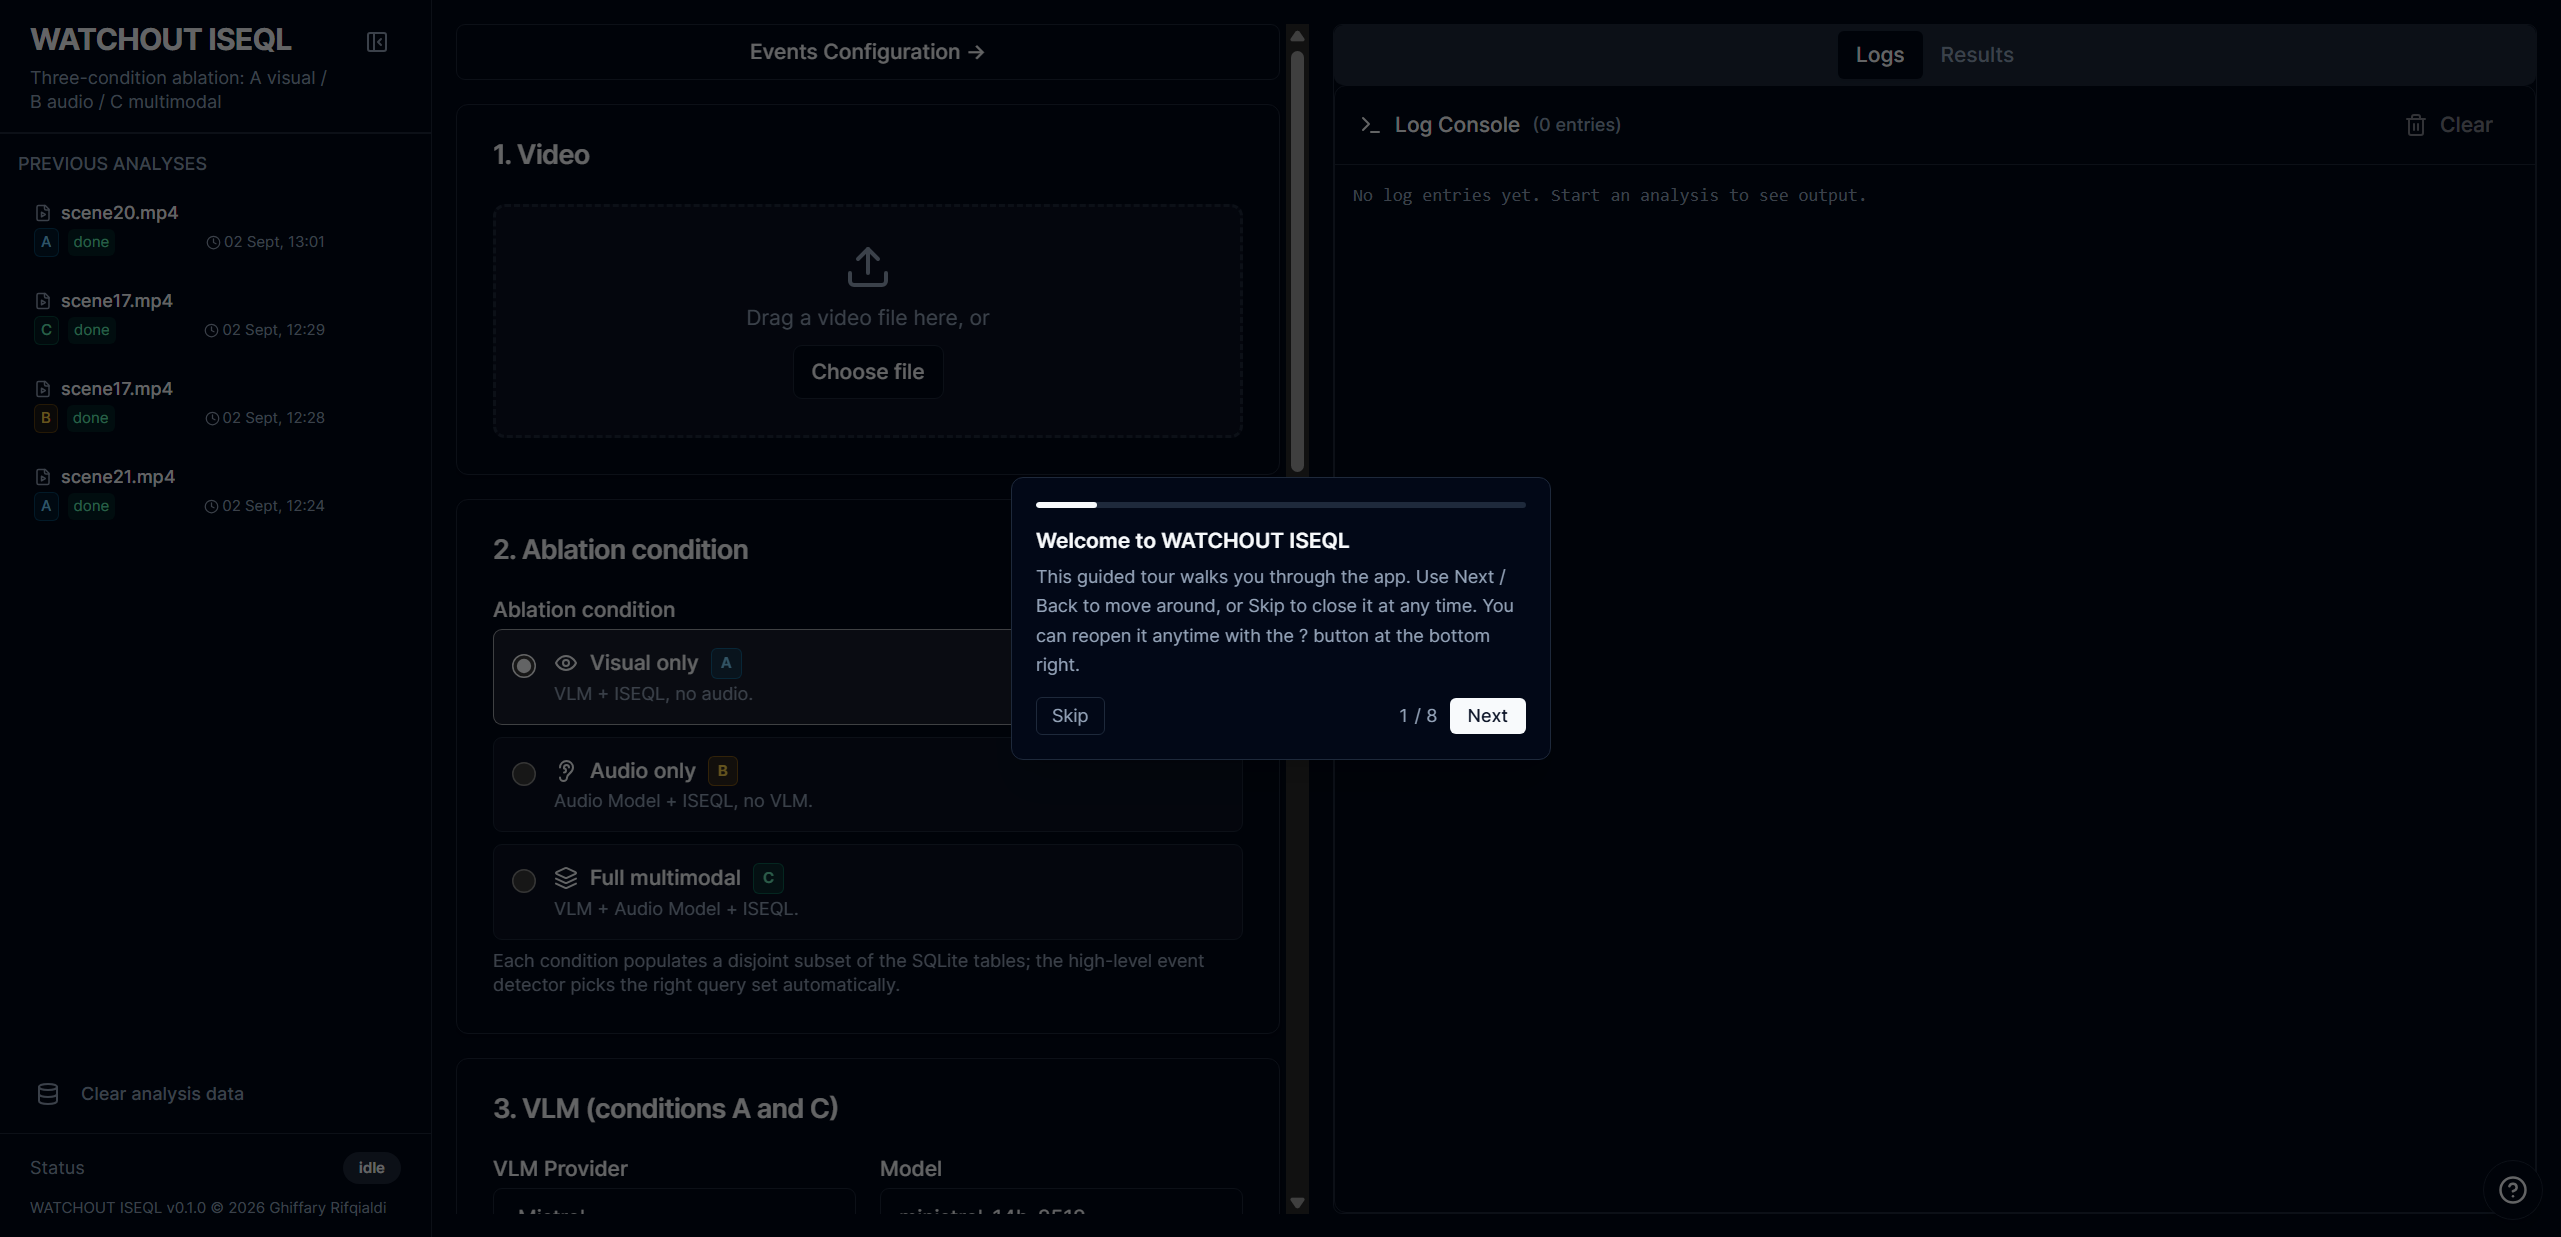
\includegraphics[width=0.92\textwidth]{Figures/appendix/tour01_landing.png}
  \caption{Welcome to WATCHOUT ISEQL: the guided tour walks you through the app.}
\end{figure}

\begin{figure}[H]
  \centering
  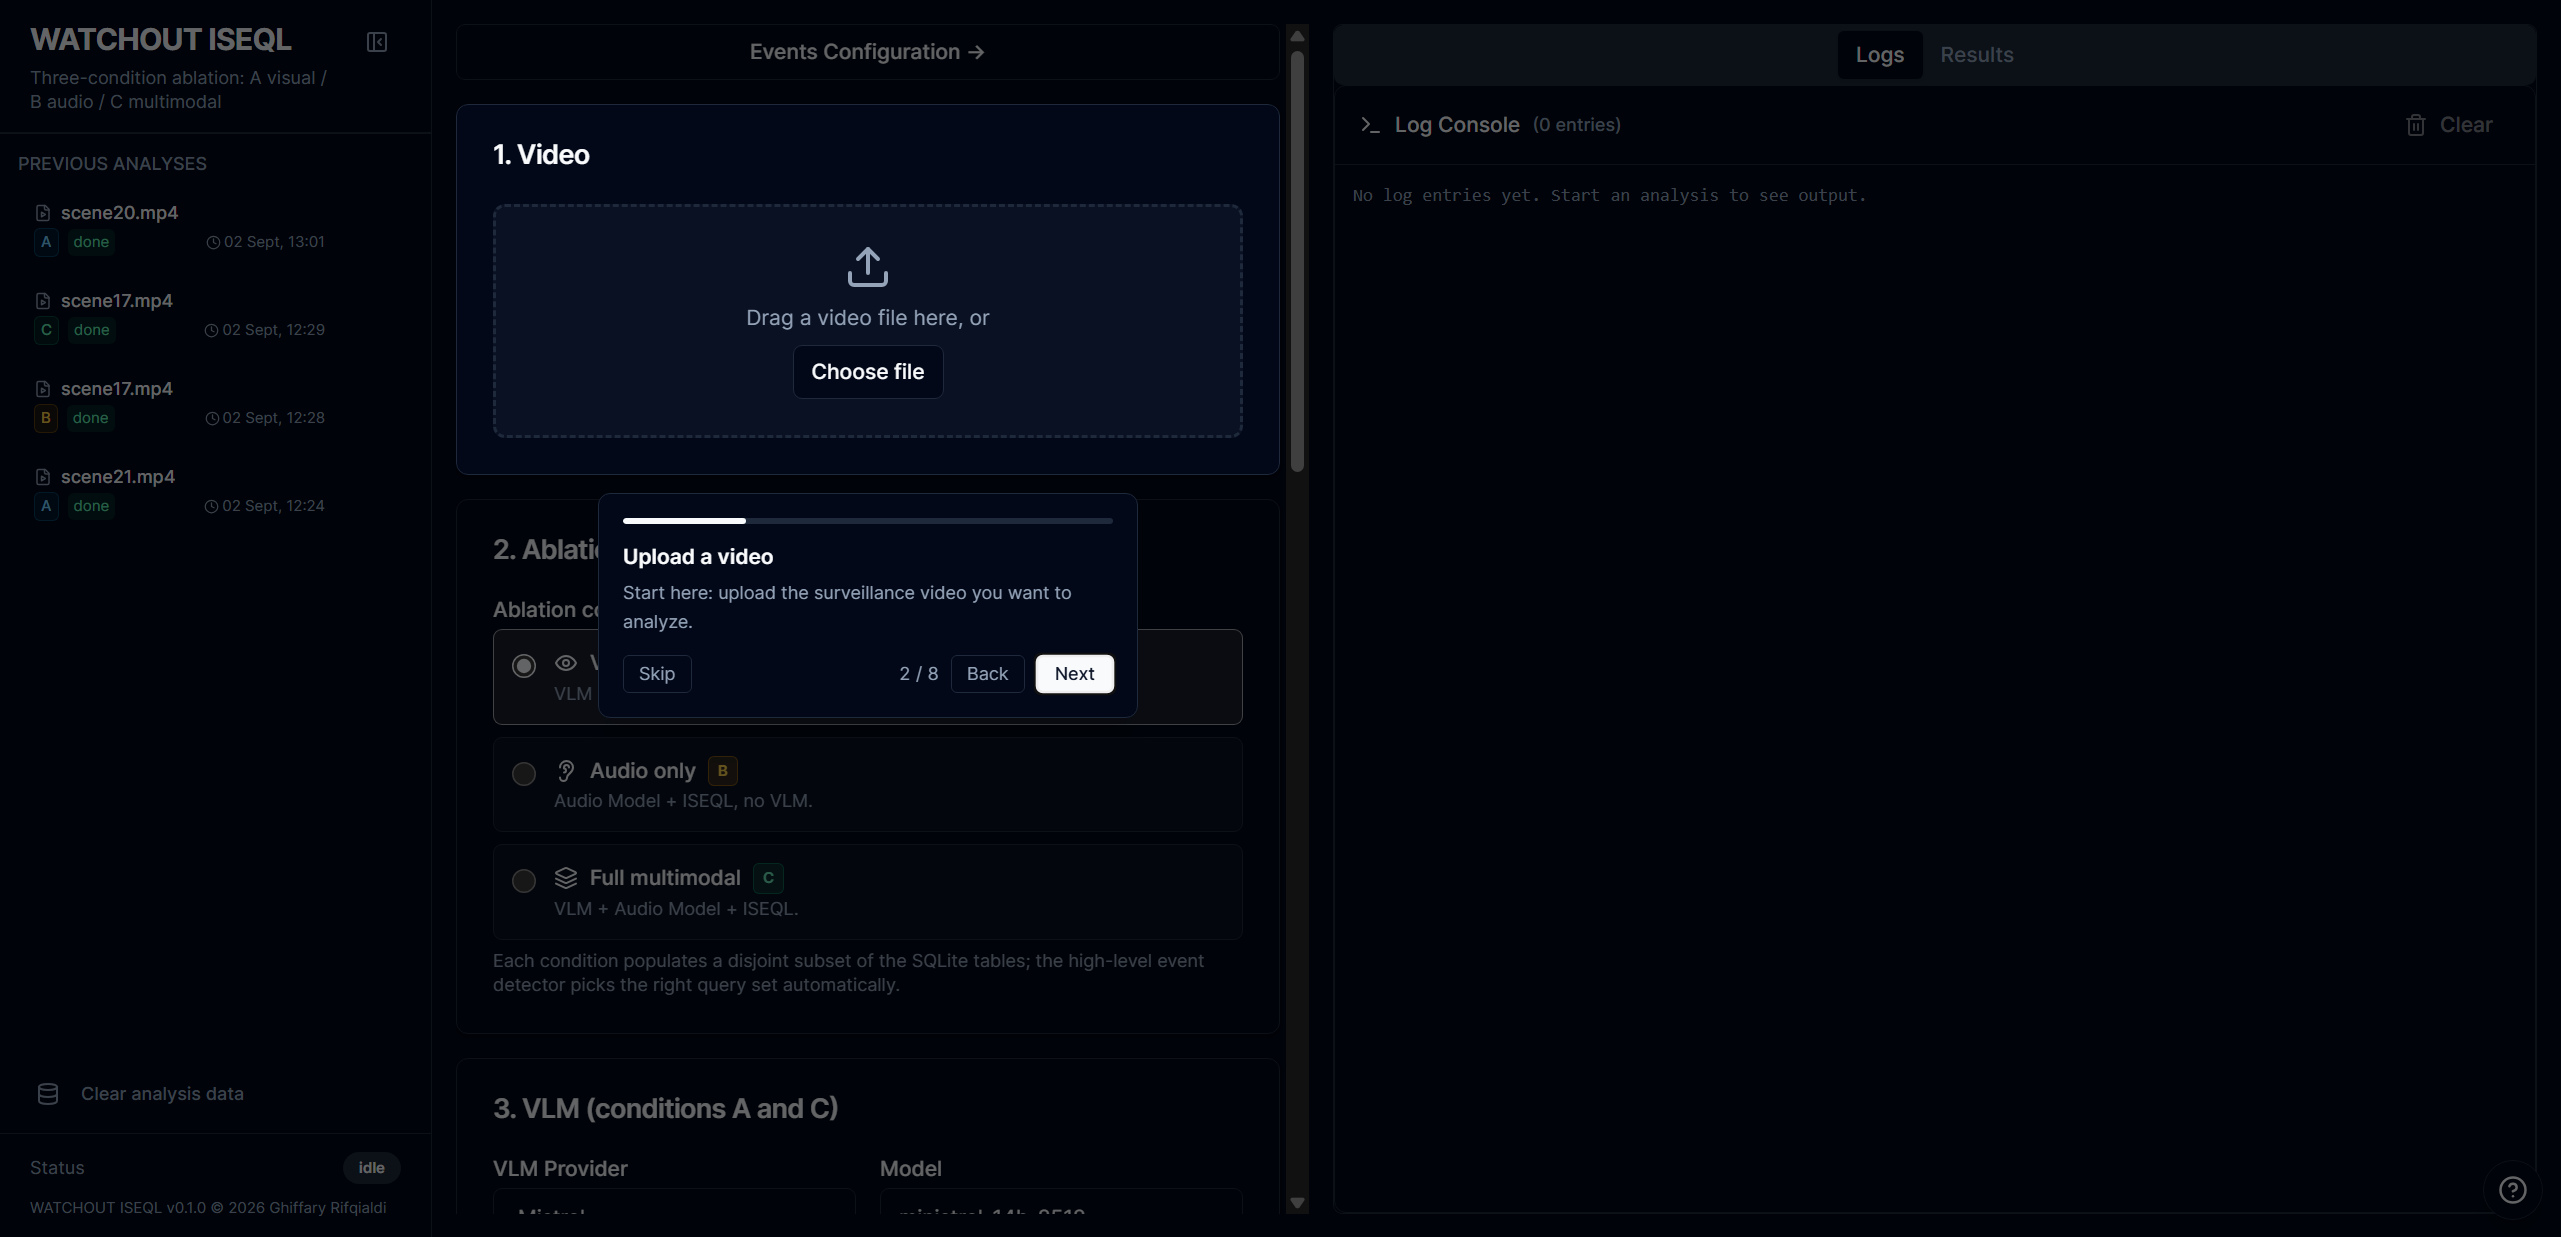
\includegraphics[width=0.92\textwidth]{Figures/appendix/tour02_upload.png}
  \caption{Upload a video: start here, upload the surveillance video you want to analyze.}
\end{figure}

\begin{figure}[H]
  \centering
  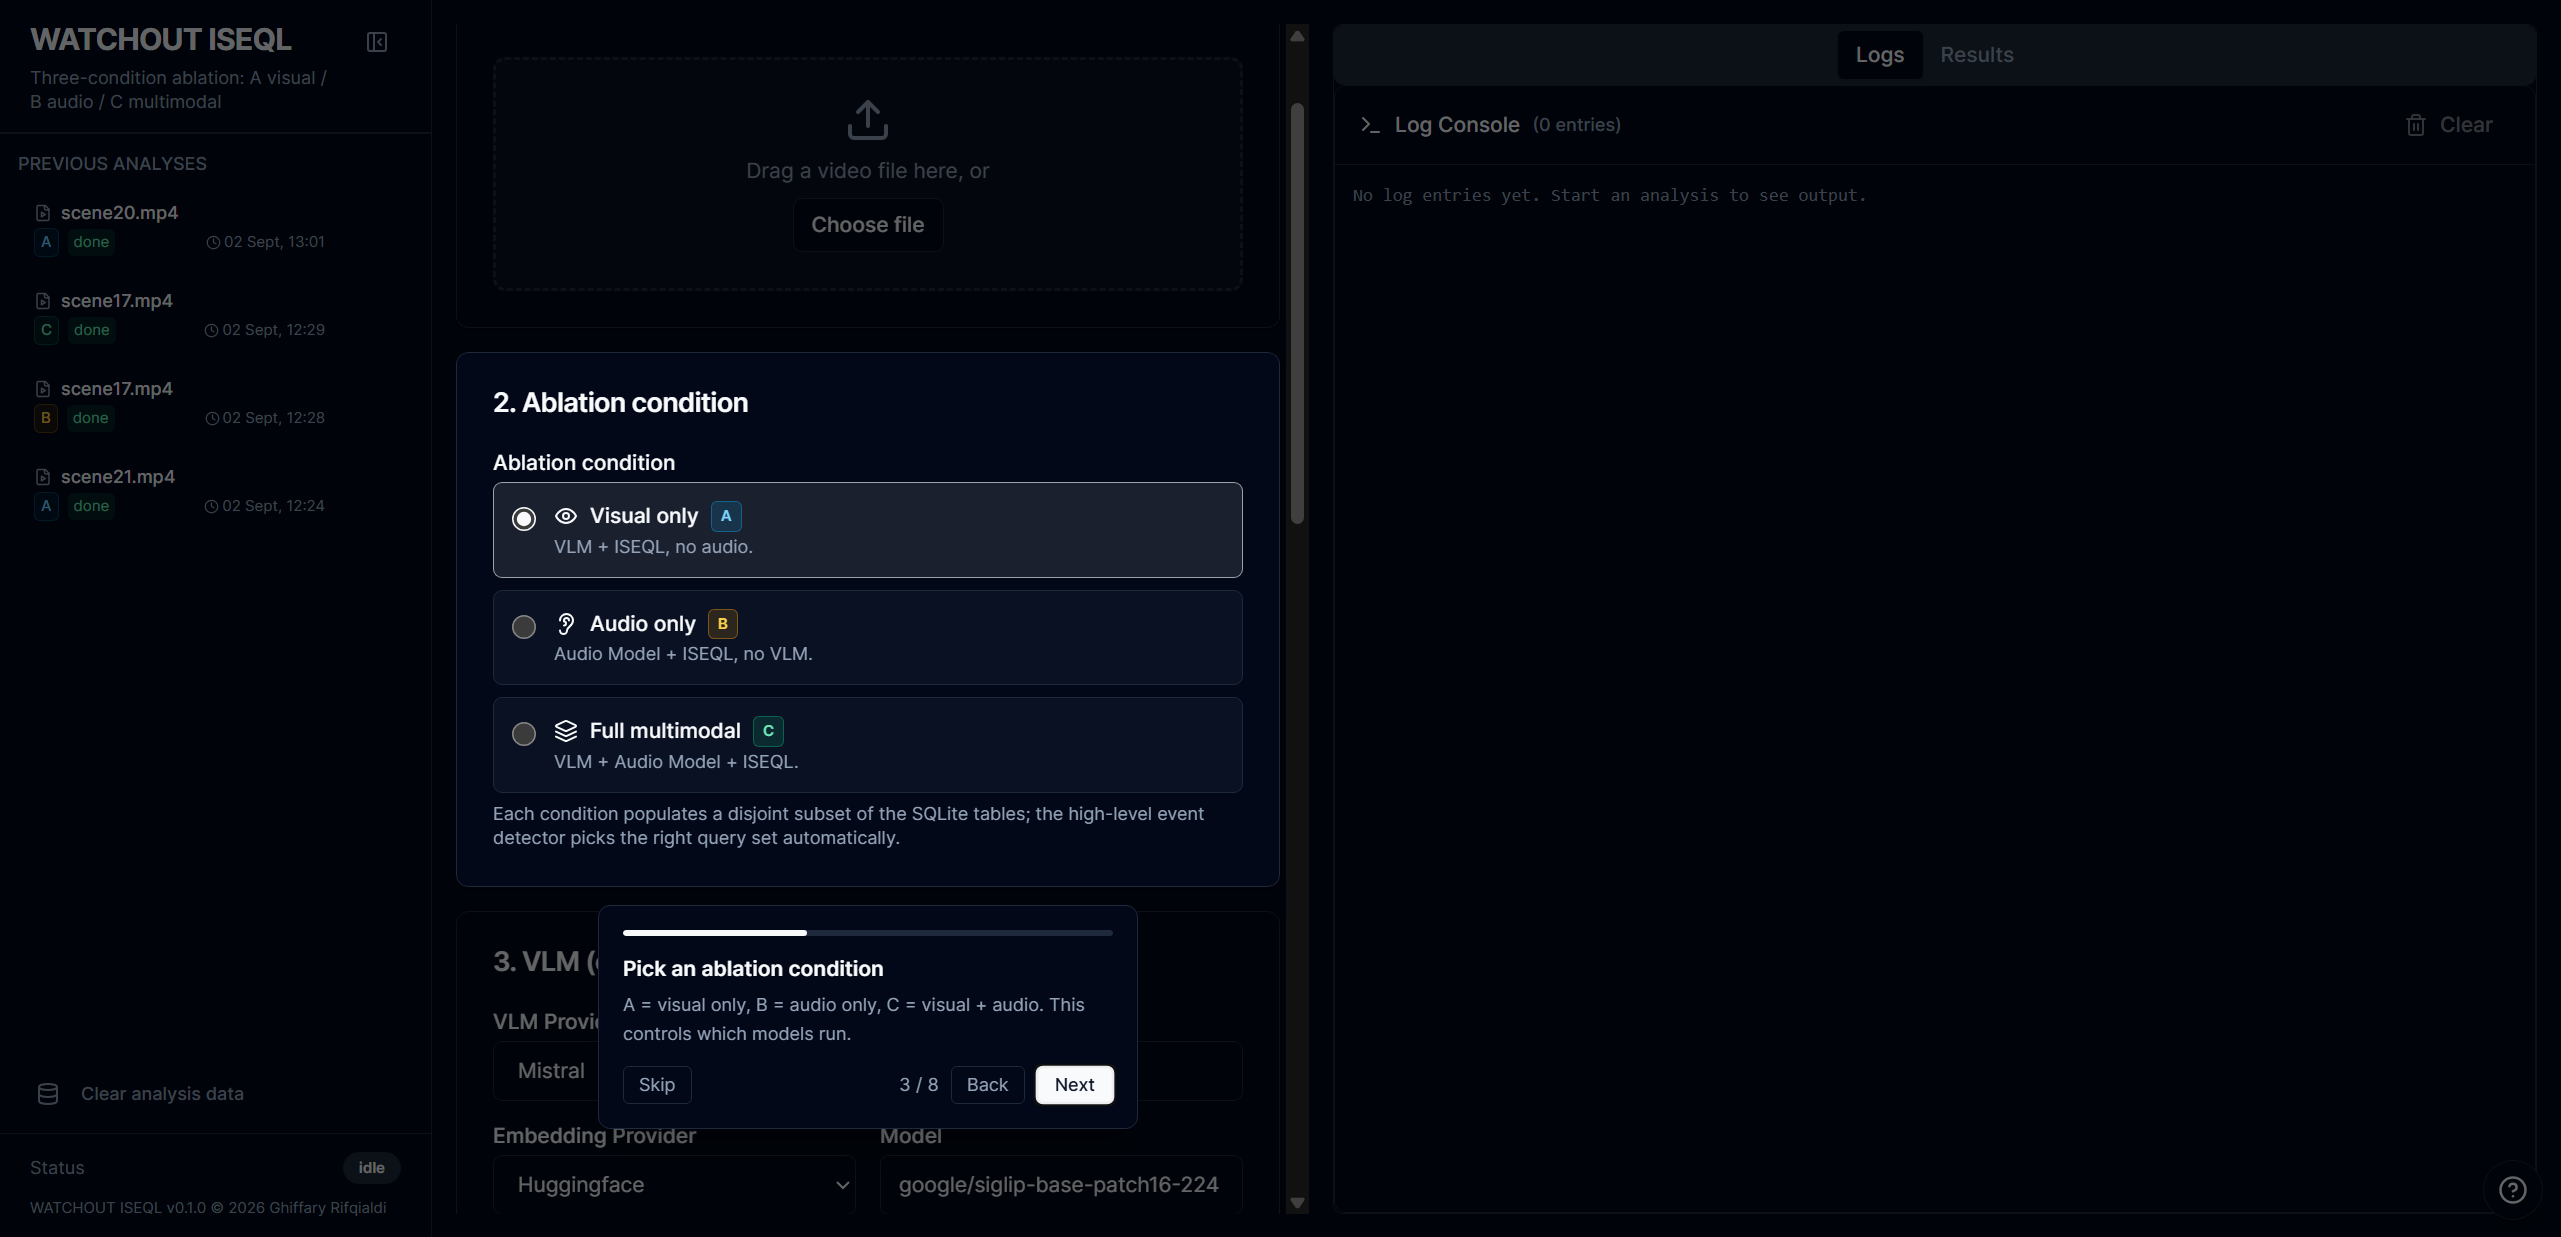
\includegraphics[width=0.92\textwidth]{Figures/appendix/tour03_condition.png}
  \caption{Pick an ablation condition: A = visual only, B = audio only, C = visual + audio.}
\end{figure}

\begin{figure}[H]
  \centering
  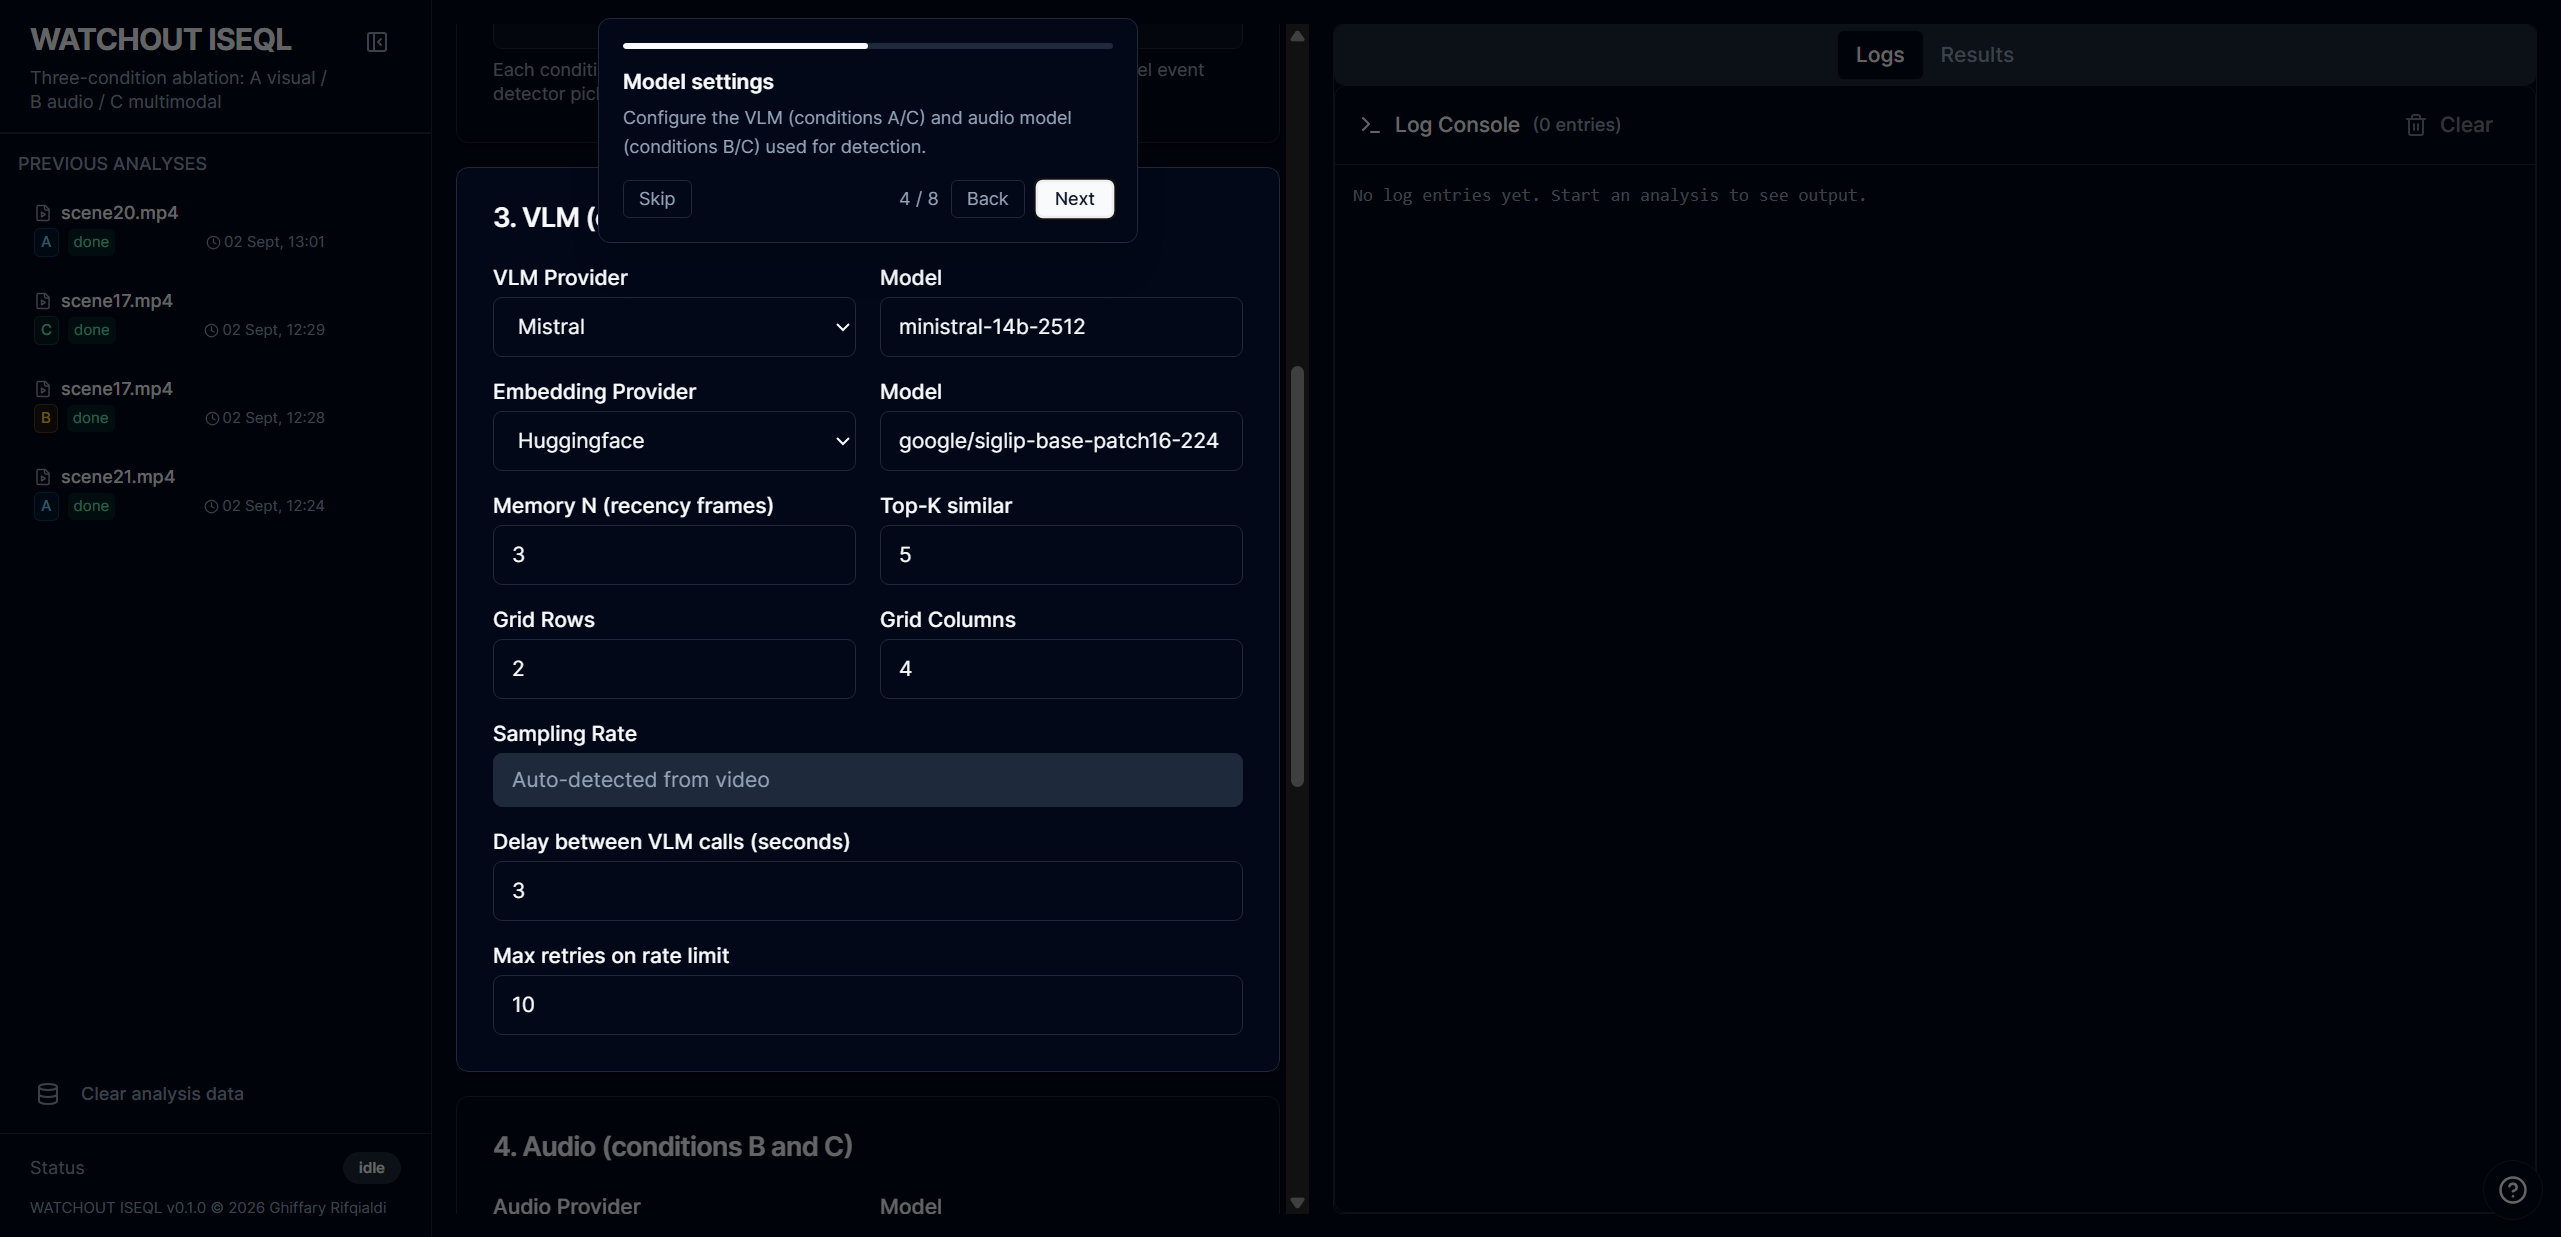
\includegraphics[width=0.92\textwidth]{Figures/appendix/tour04_model.png}
  \caption{Model settings: configure the VLM (conditions A/C) and audio model (conditions B/C).}
\end{figure}

\begin{figure}[H]
  \centering
  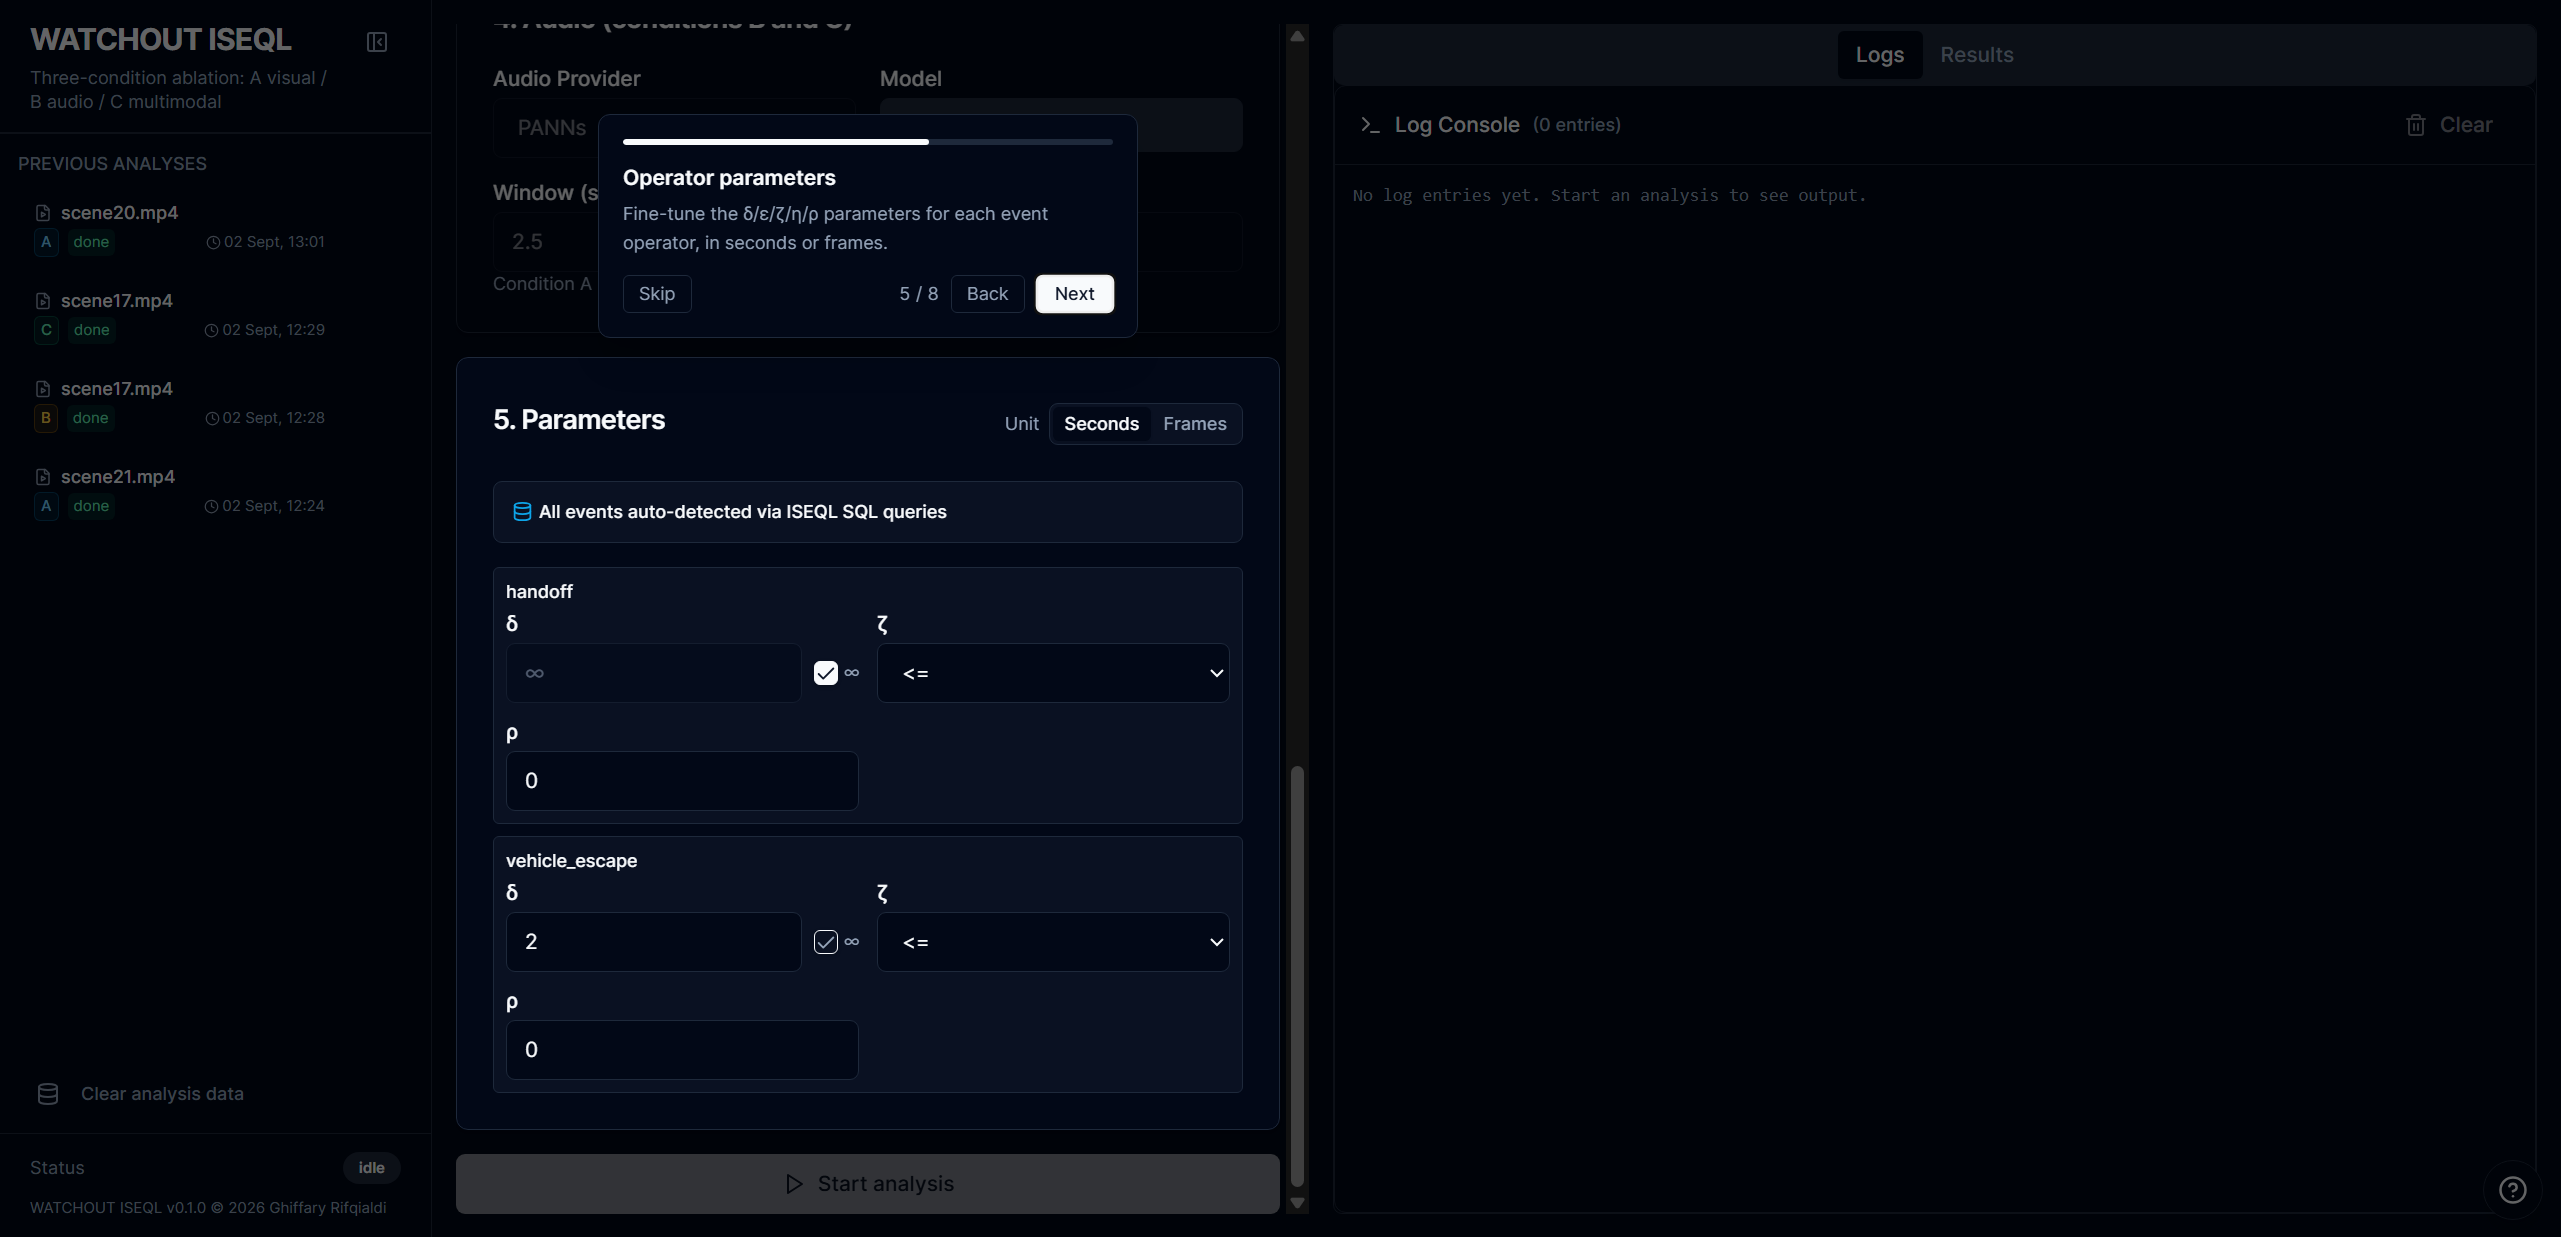
\includegraphics[width=0.92\textwidth]{Figures/appendix/tour05_params.png}
  \caption{Operator parameters: fine-tune the $\delta$, $\epsilon$, $\zeta$, $\eta$, $\rho$ parameters for each event operator.}
\end{figure}

\begin{figure}[H]
  \centering
  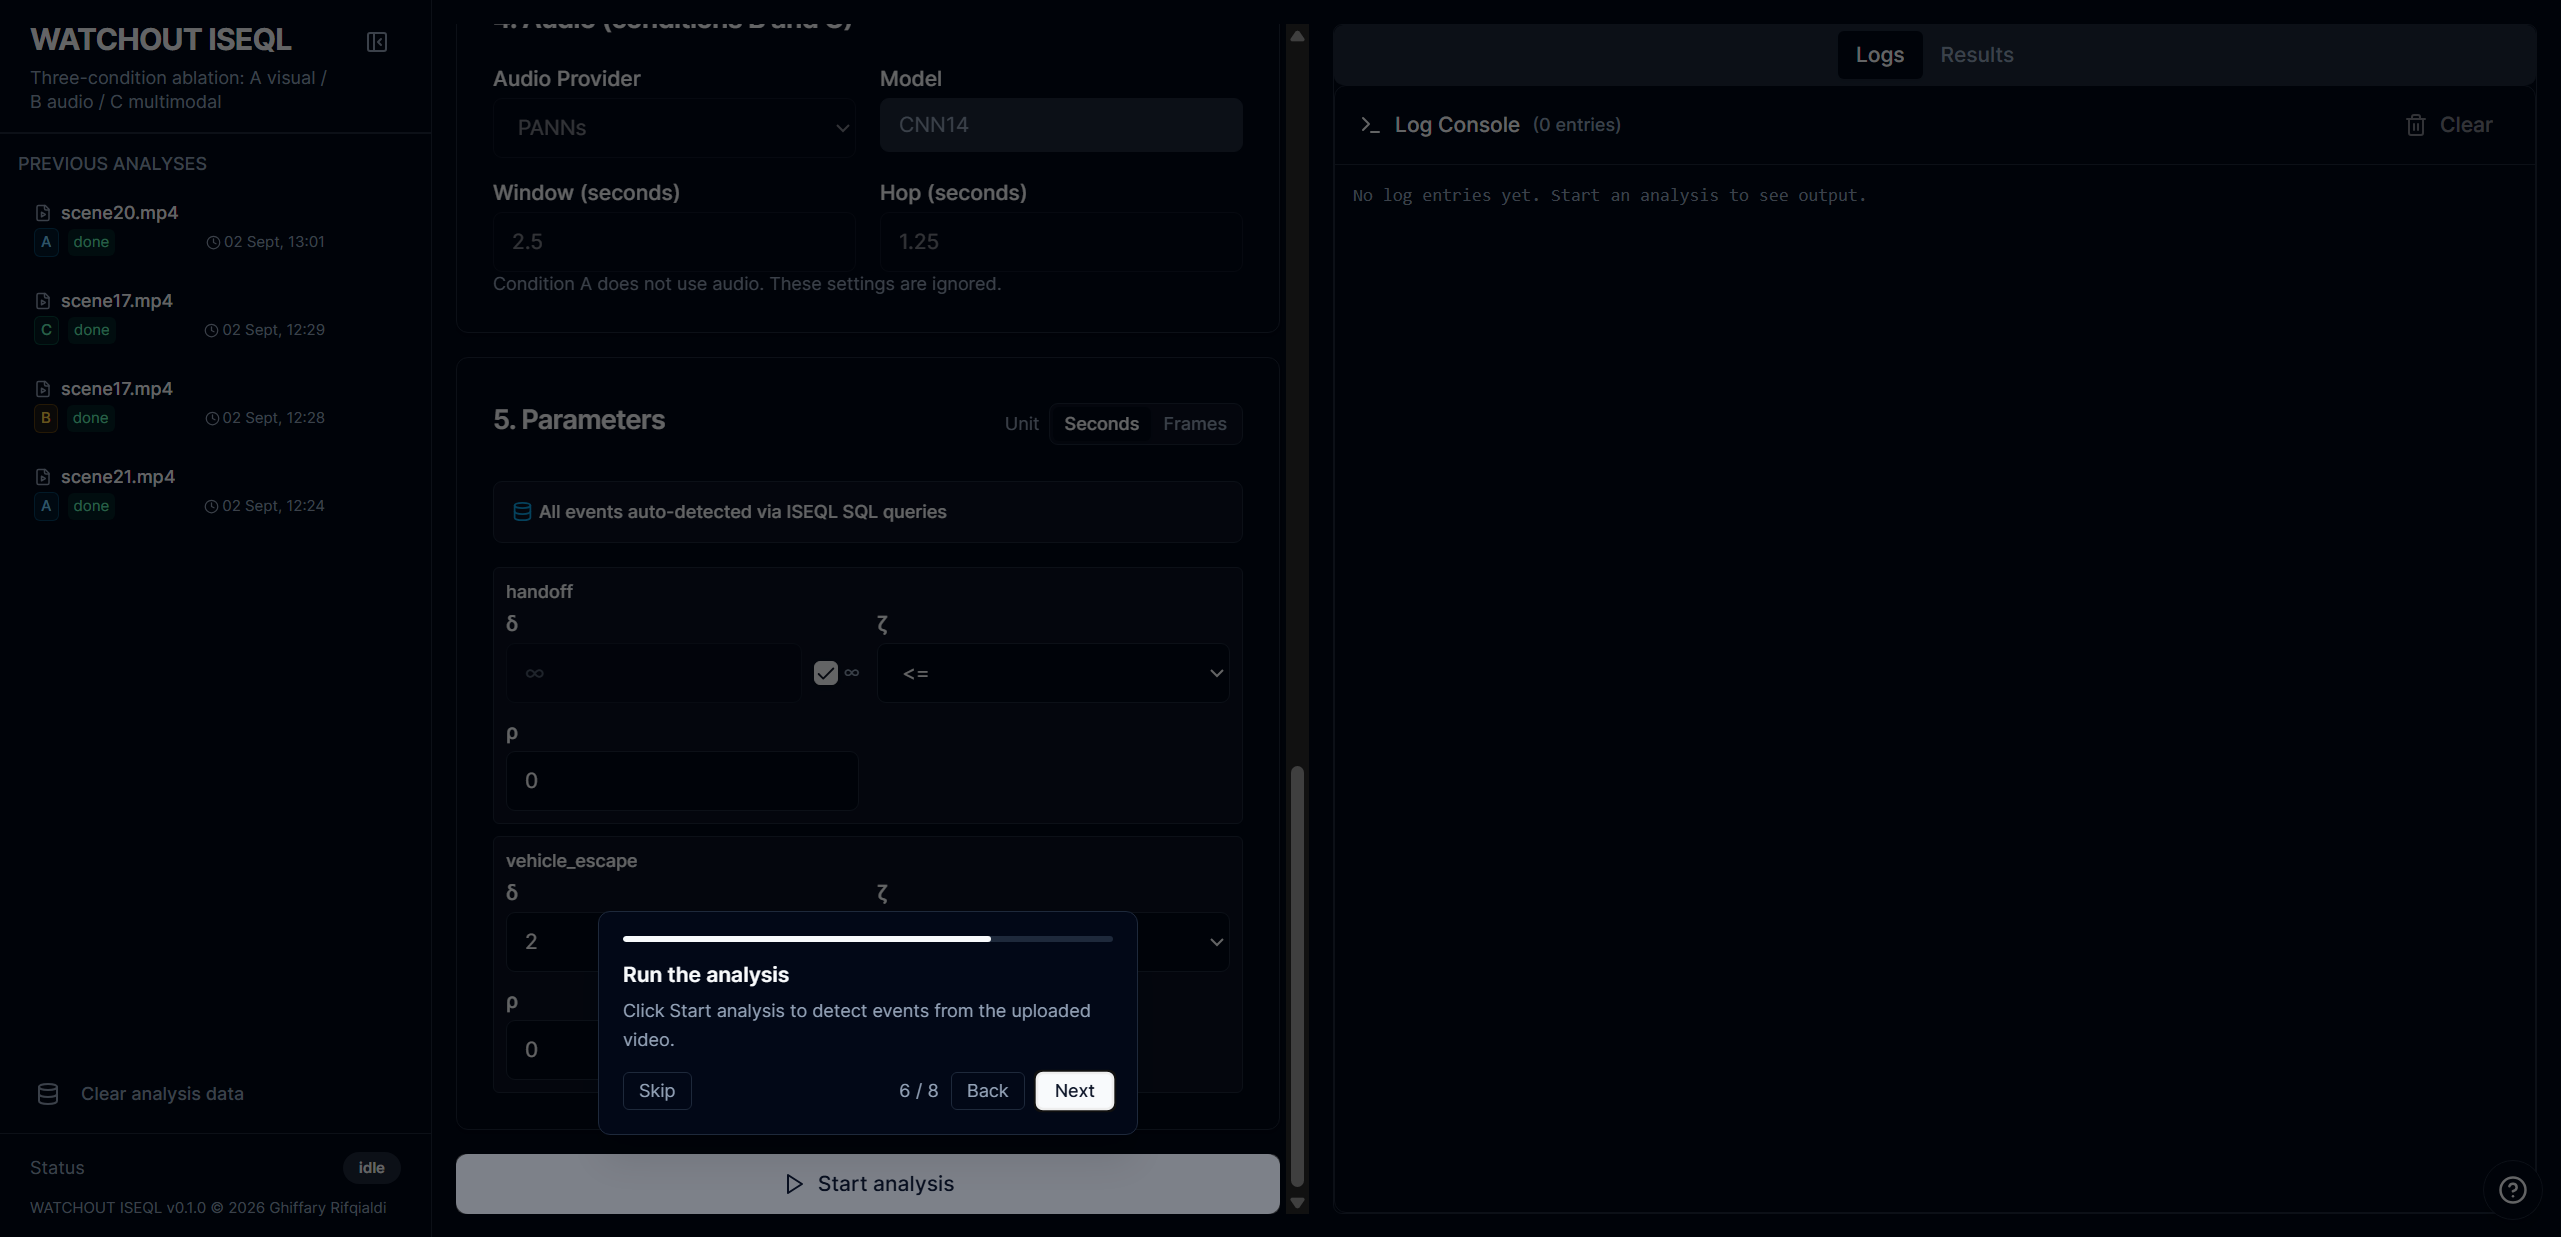
\includegraphics[width=0.92\textwidth]{Figures/appendix/tour06_run.png}
  \caption{Run the analysis: click Start analysis to detect events from the uploaded video.}
\end{figure}

\begin{figure}[H]
  \centering
  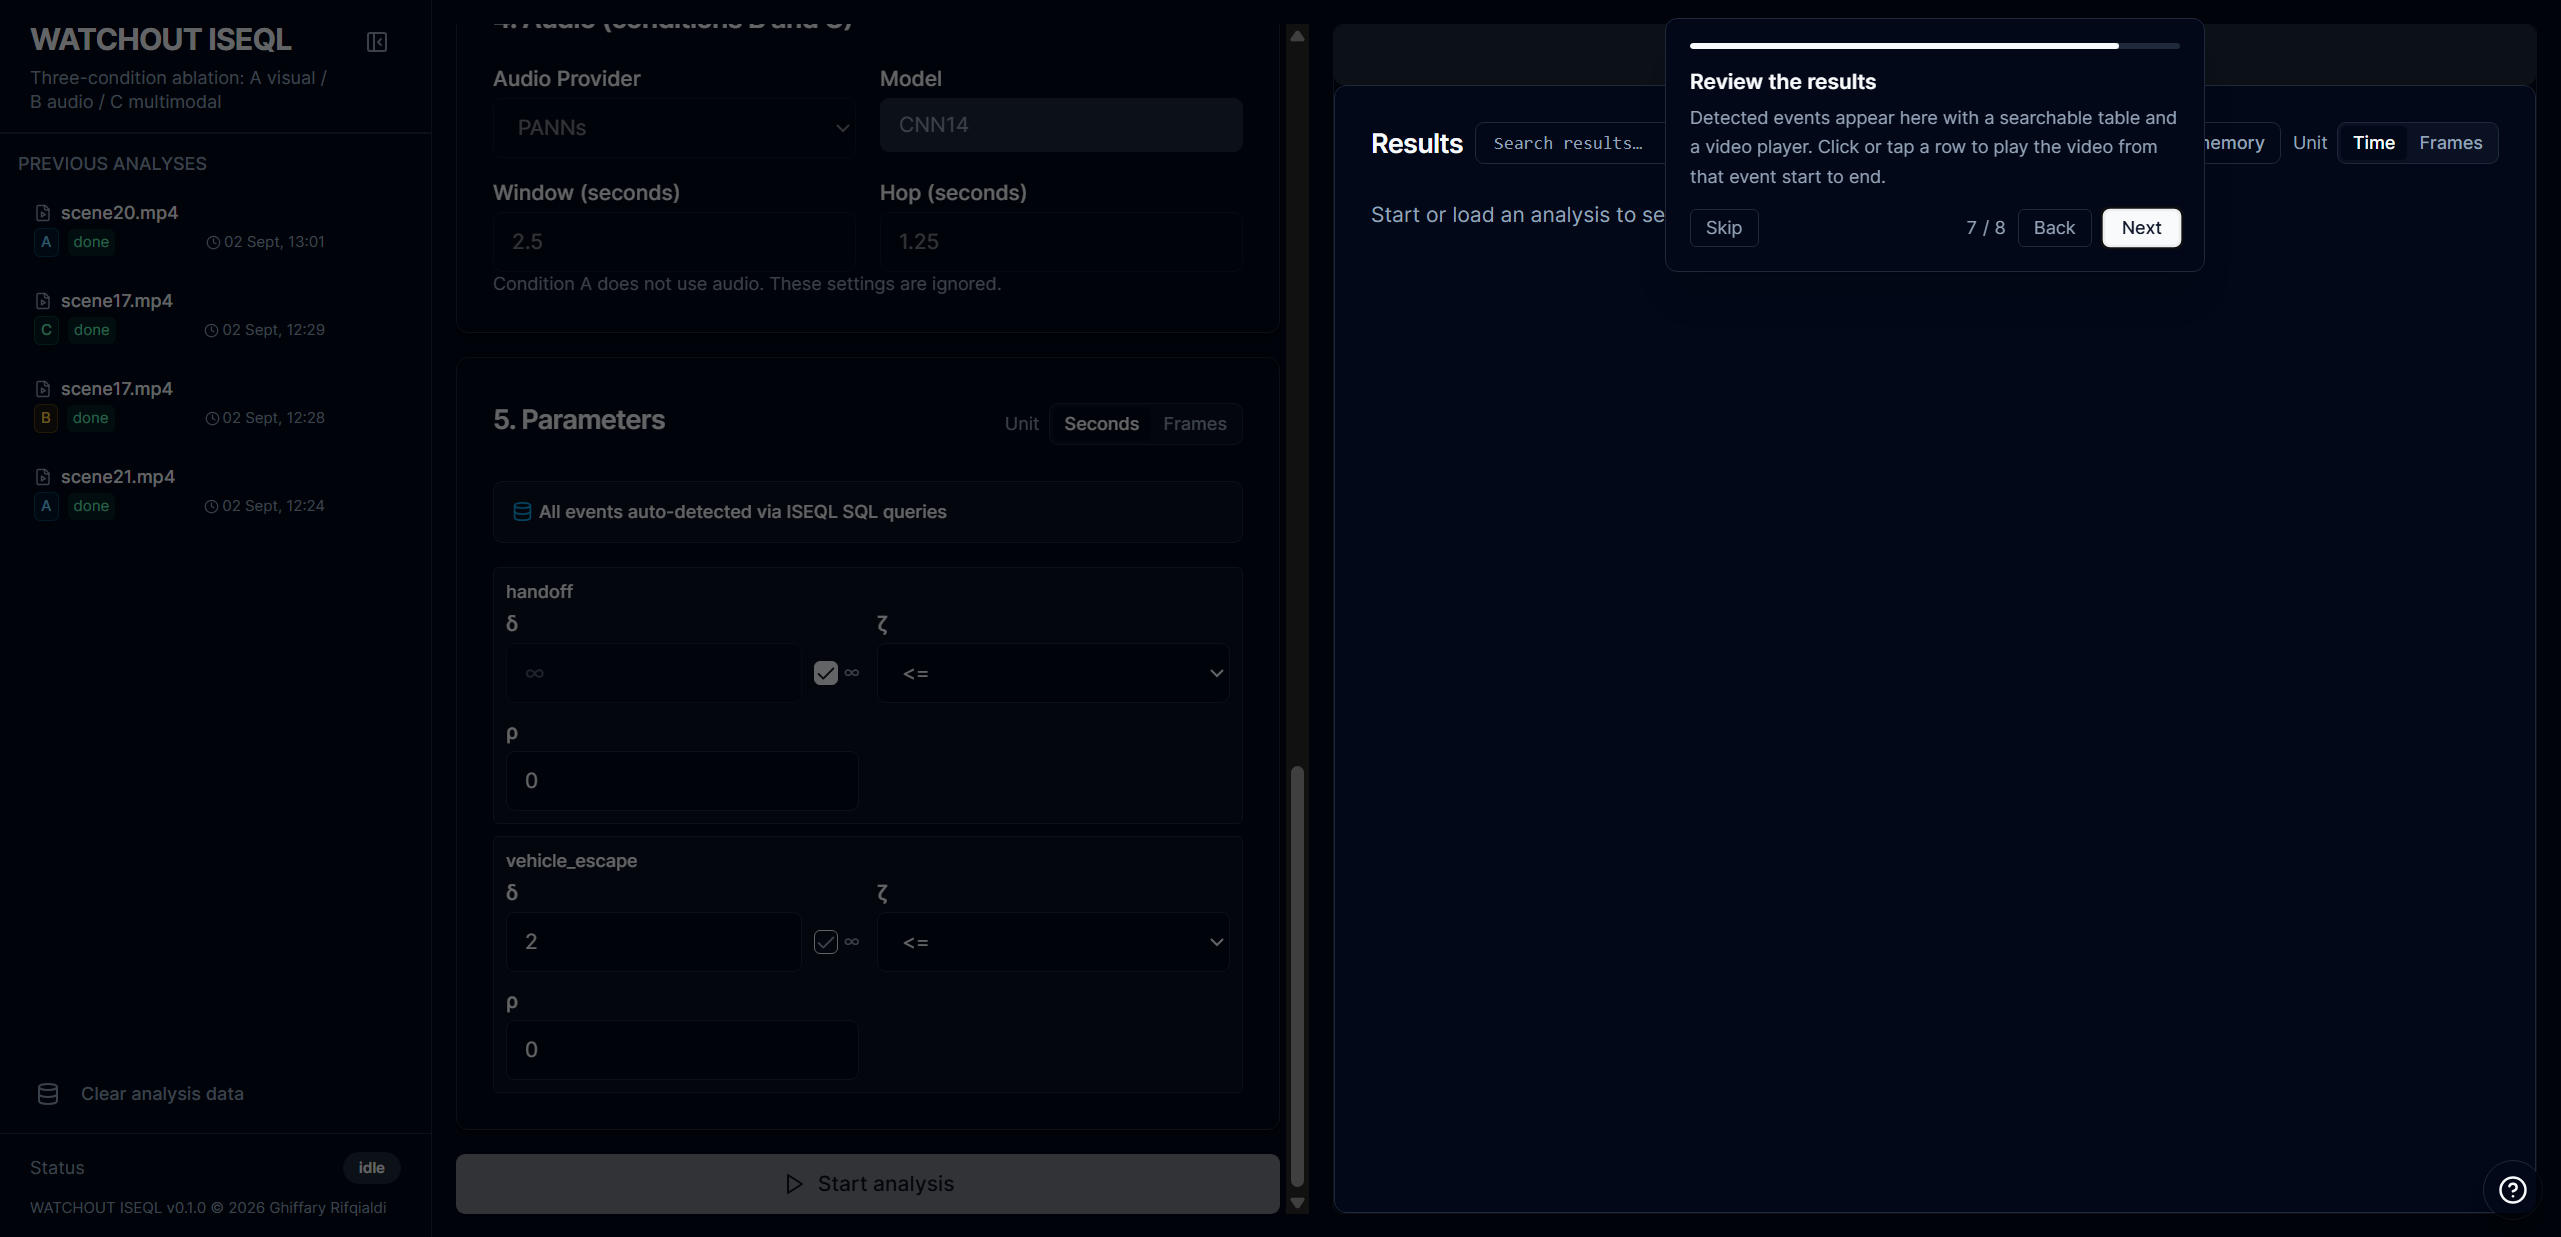
\includegraphics[width=0.92\textwidth]{Figures/appendix/tour07_results.png}
  \caption{Review the results: detected events appear in a searchable table with a video player.}
\end{figure}

\begin{figure}[H]
  \centering
  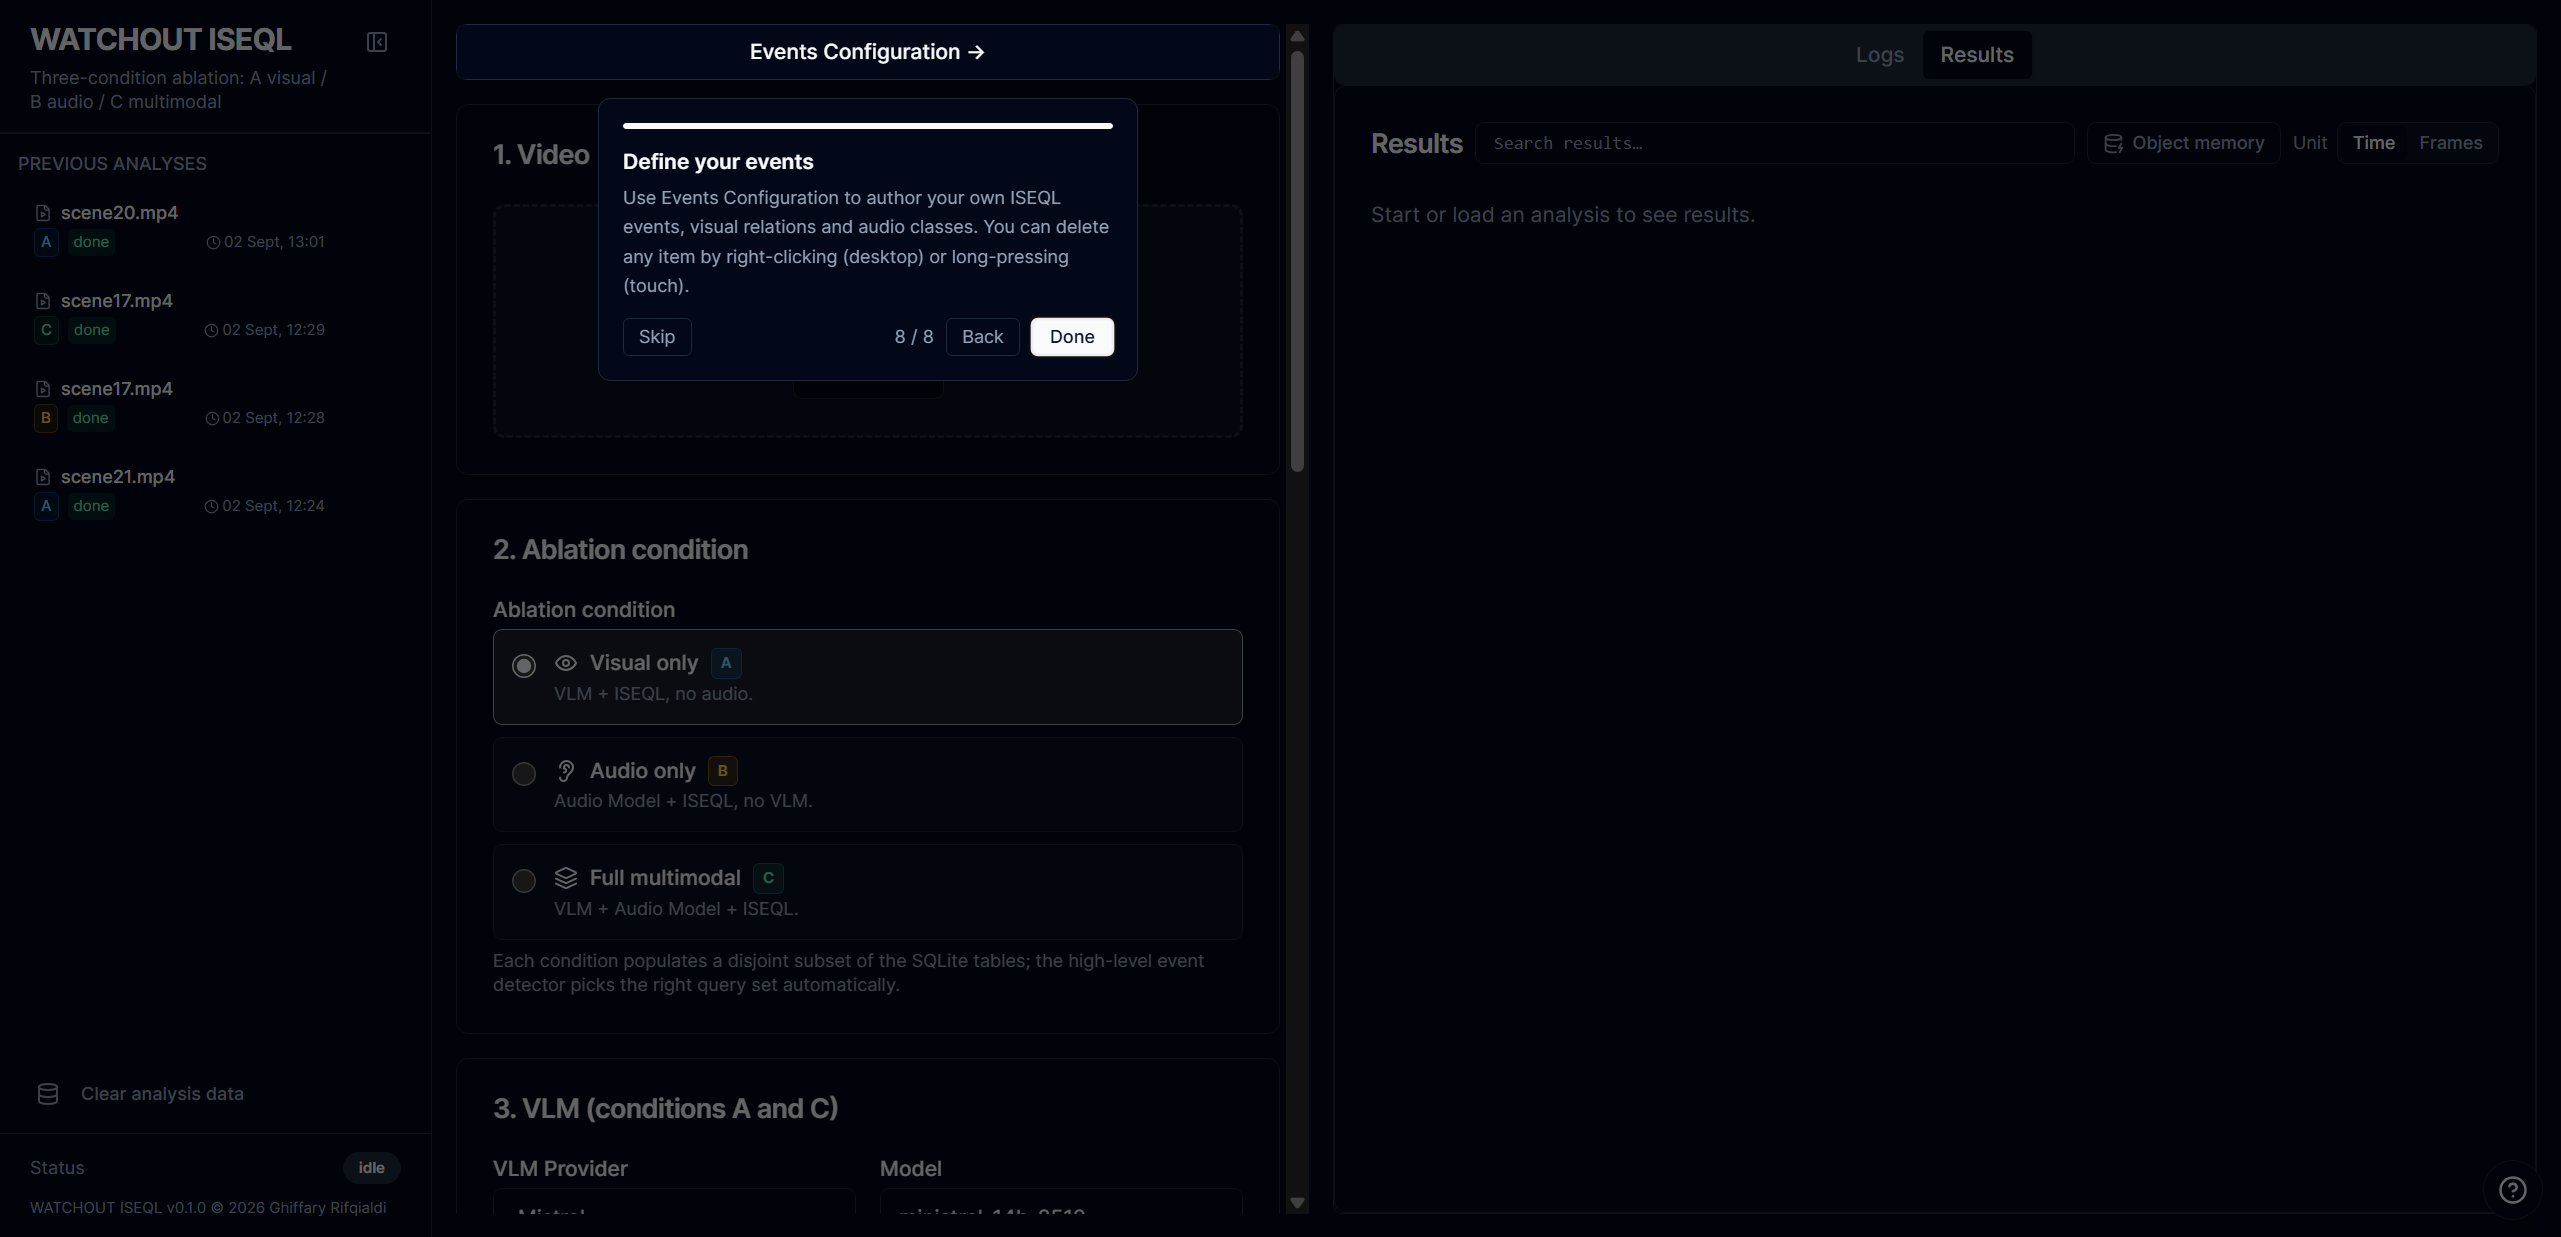
\includegraphics[width=0.92\textwidth]{Figures/appendix/tour08_define_events.png}
  \caption{Define your events: use Events Configuration to author ISEQL events, visual relations and audio classes.}
\end{figure}

\section{Event Configuration}

Events, visual relations, and audio classes are all user-configurable through the web interface. The following figures show the predicates (visual relations and audio classes) and the event authoring flow.

\begin{figure}[H]
  \centering
  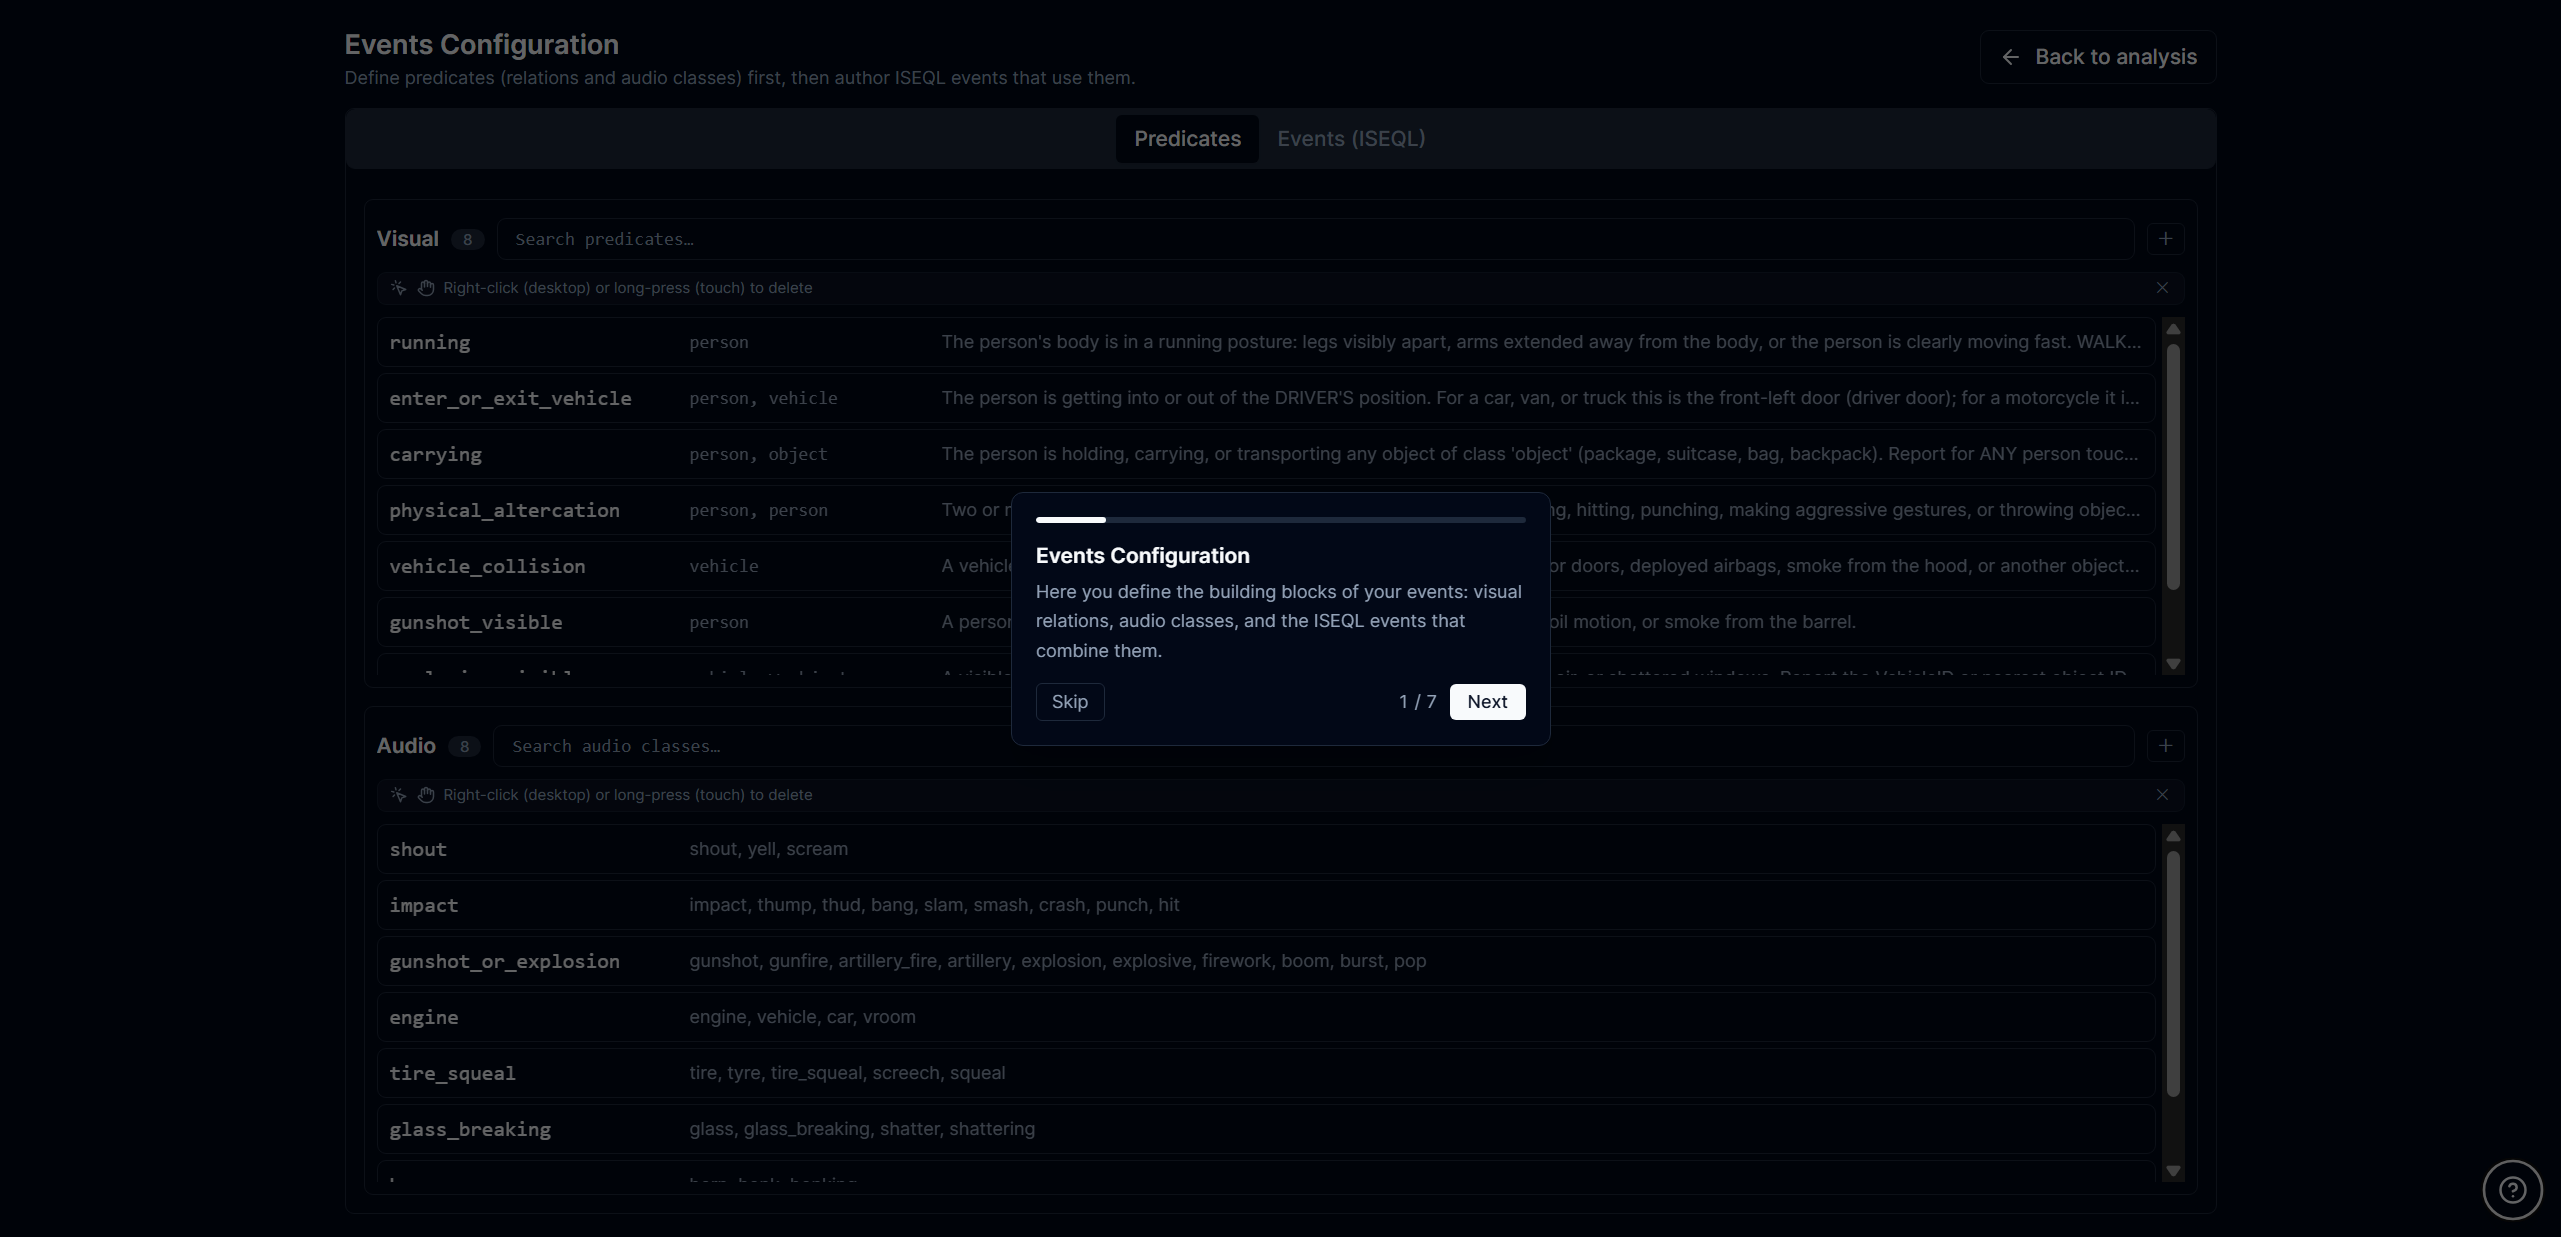
\includegraphics[width=0.92\textwidth]{Figures/appendix/cfg01_predicates.png}
  \caption{Event Configuration: define the building blocks of your events.}
\end{figure}

\begin{figure}[H]
  \centering
  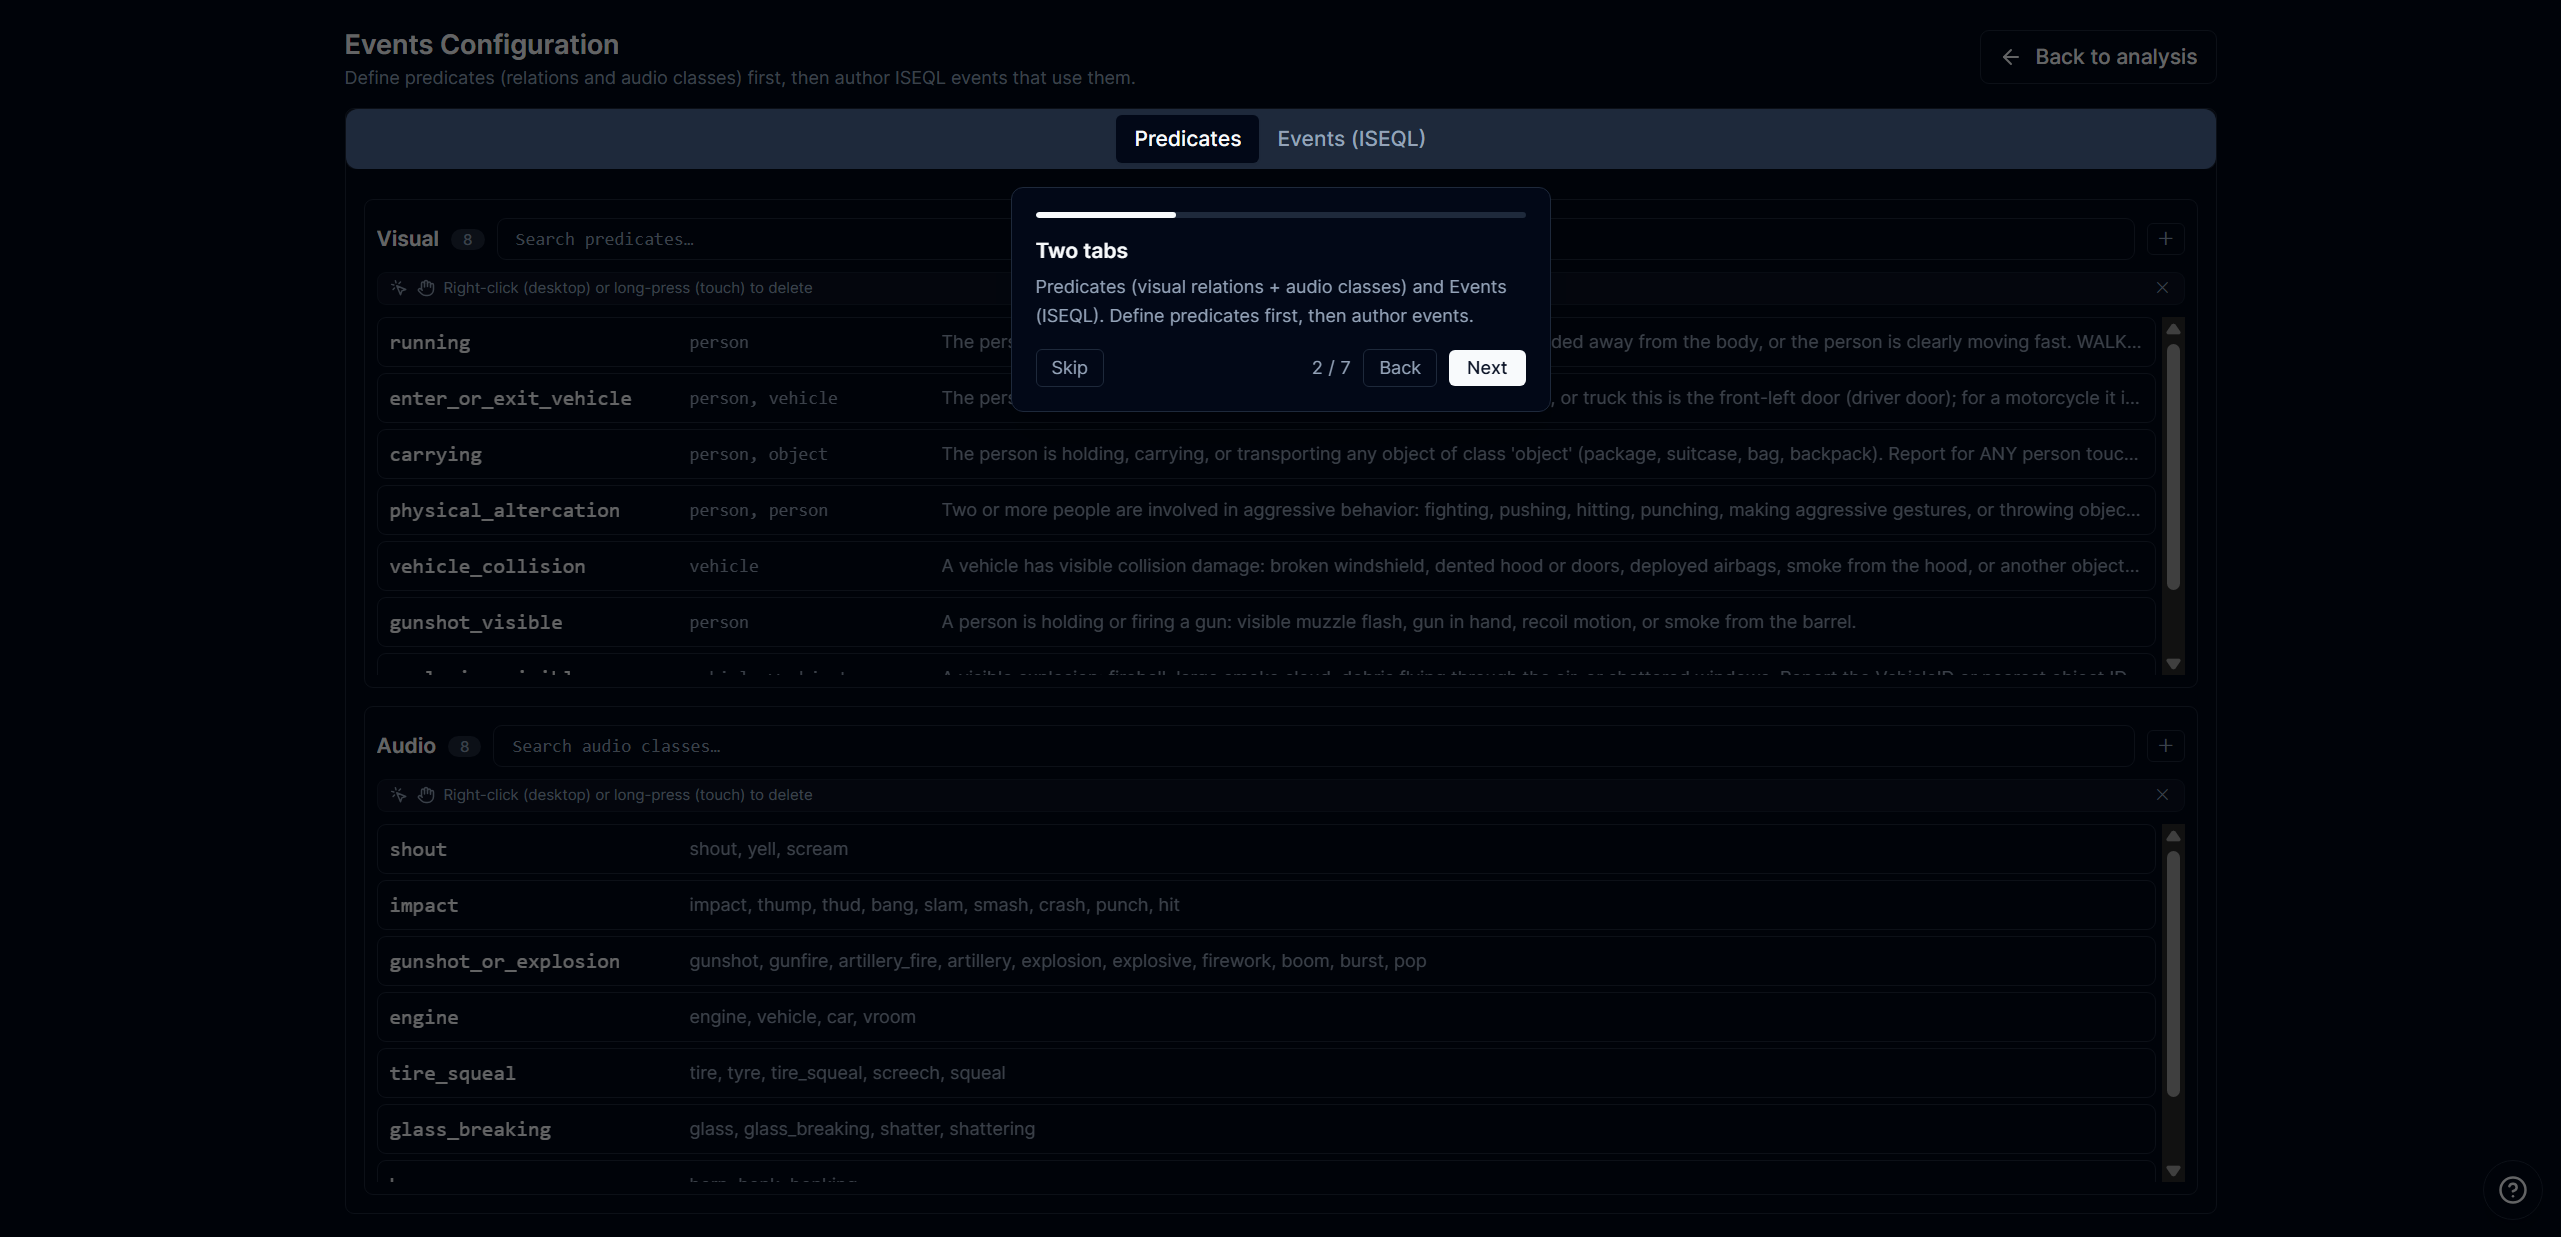
\includegraphics[width=0.92\textwidth]{Figures/appendix/cfg02_predicates_tabs.png}
  \caption{Two tabs: Predicates (visual relations + audio classes) and Events (ISEQL).}
\end{figure}

\begin{figure}[H]
  \centering
  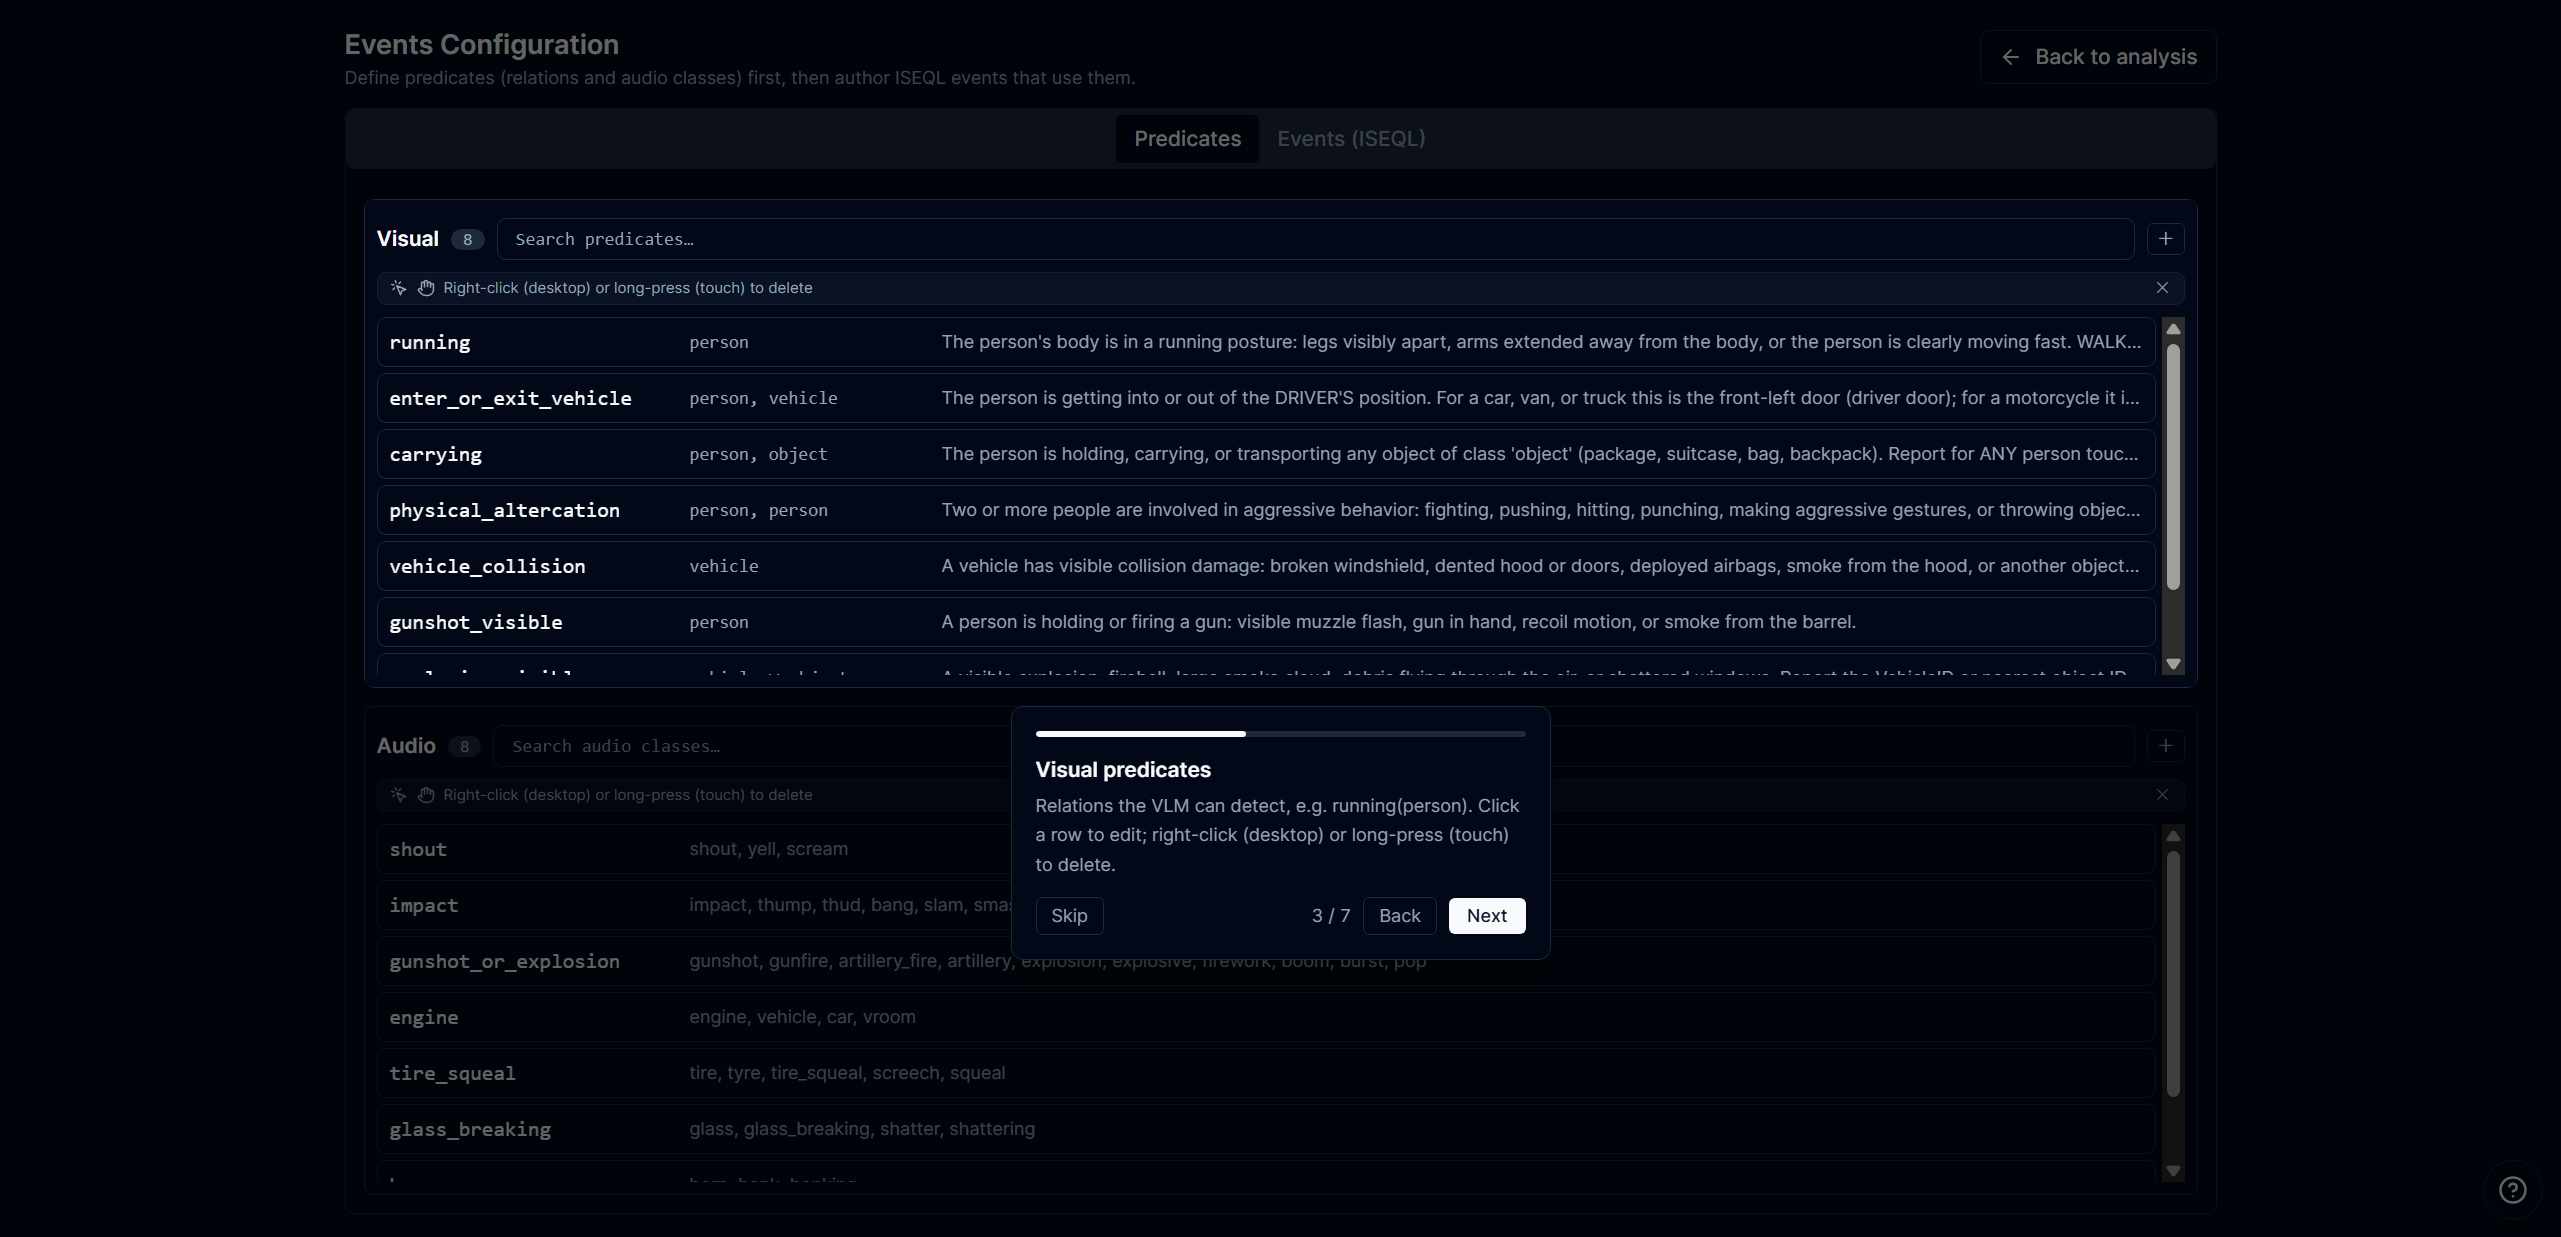
\includegraphics[width=0.92\textwidth]{Figures/appendix/cfg03_visual.png}
  \caption{Visual predicates: relations the VLM can detect, e.g. running(person).}
\end{figure}

\begin{figure}[H]
  \centering
  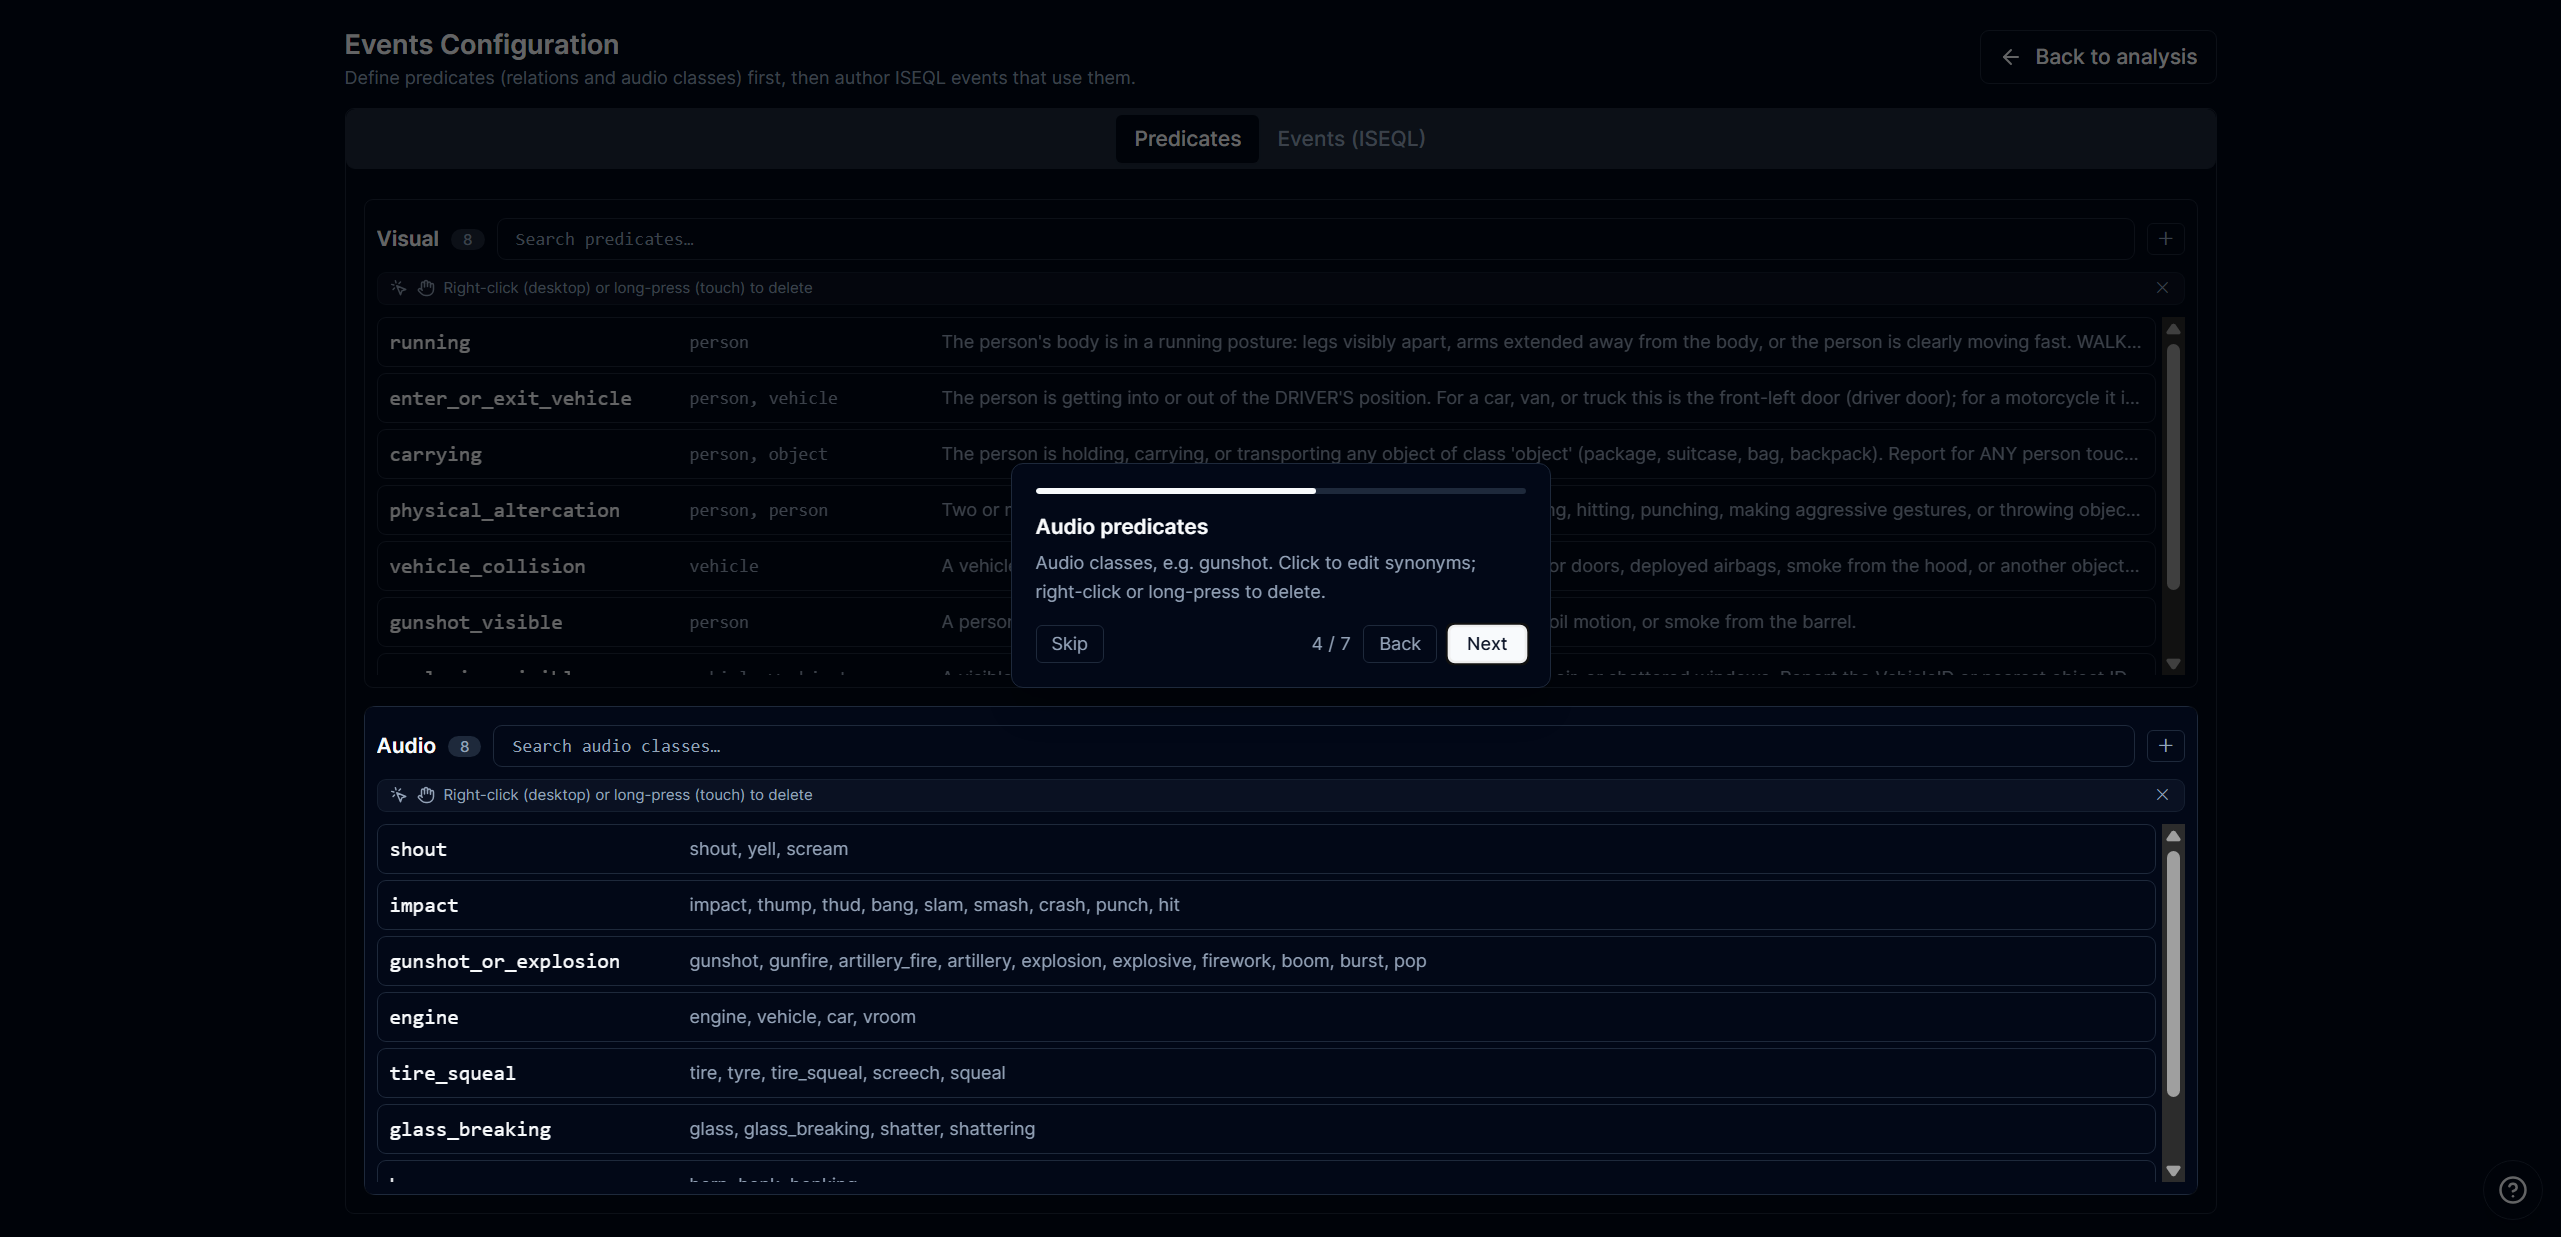
\includegraphics[width=0.92\textwidth]{Figures/appendix/cfg04_audio.png}
  \caption{Audio predicates: audio classes, e.g. gunshot.}
\end{figure}

\begin{figure}[H]
  \centering
  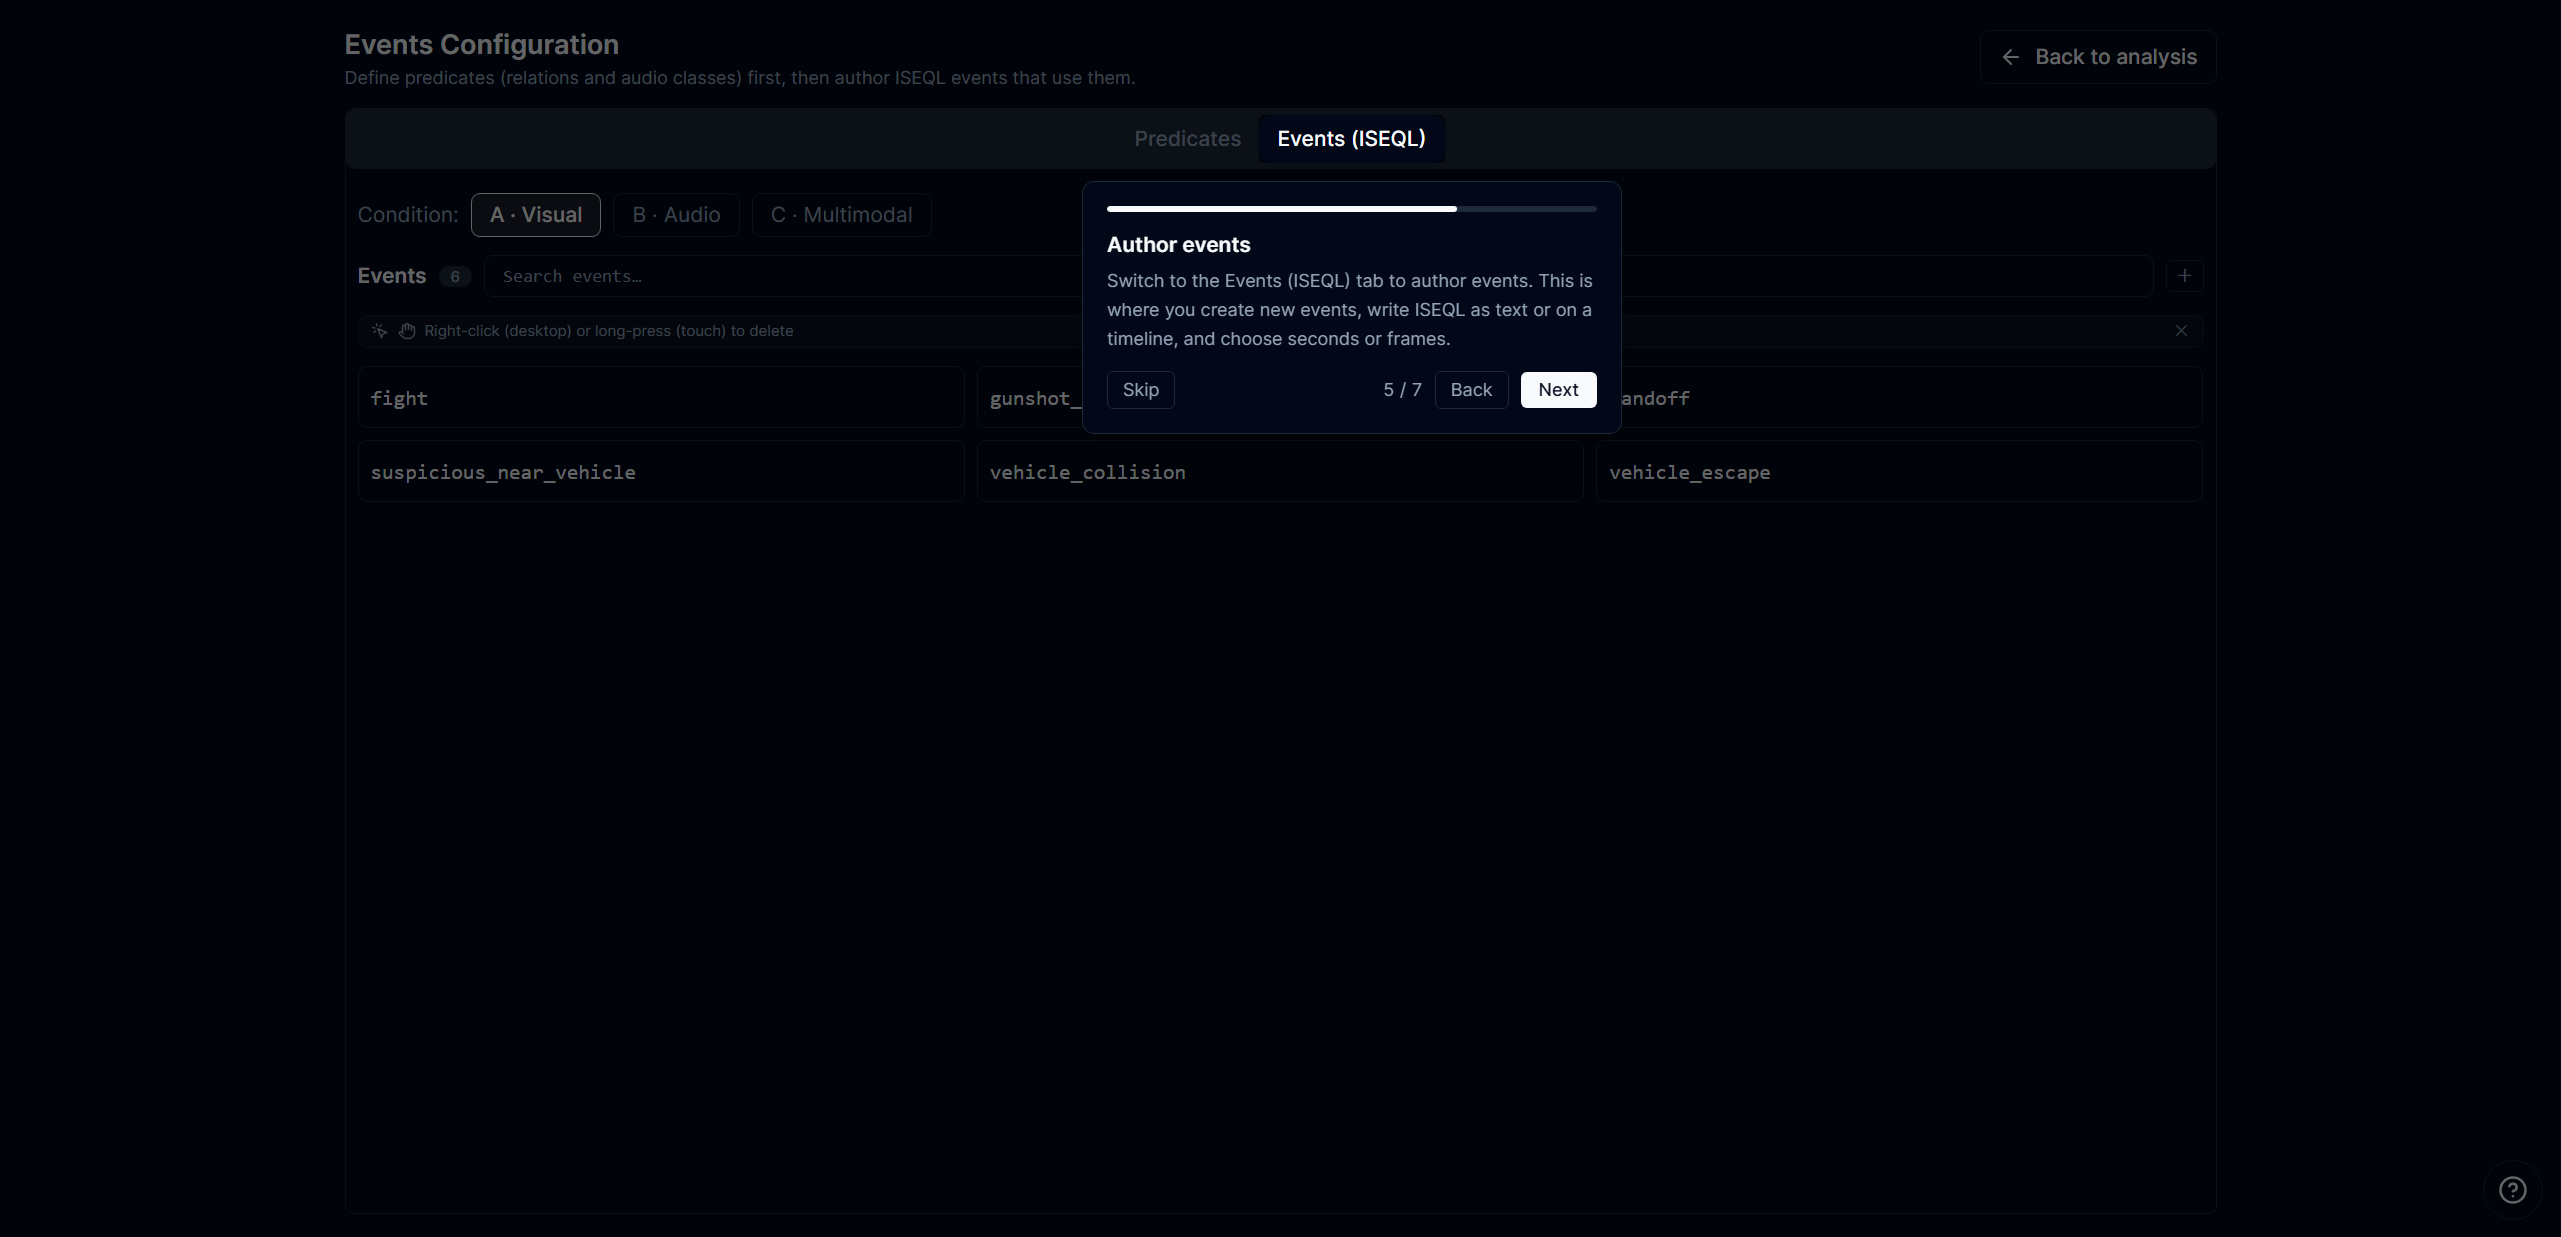
\includegraphics[width=0.92\textwidth]{Figures/appendix/cfg05_events_tab.png}
  \caption{Author events: switch to the Events (ISEQL) tab to author events.}
\end{figure}

\begin{figure}[H]
  \centering
  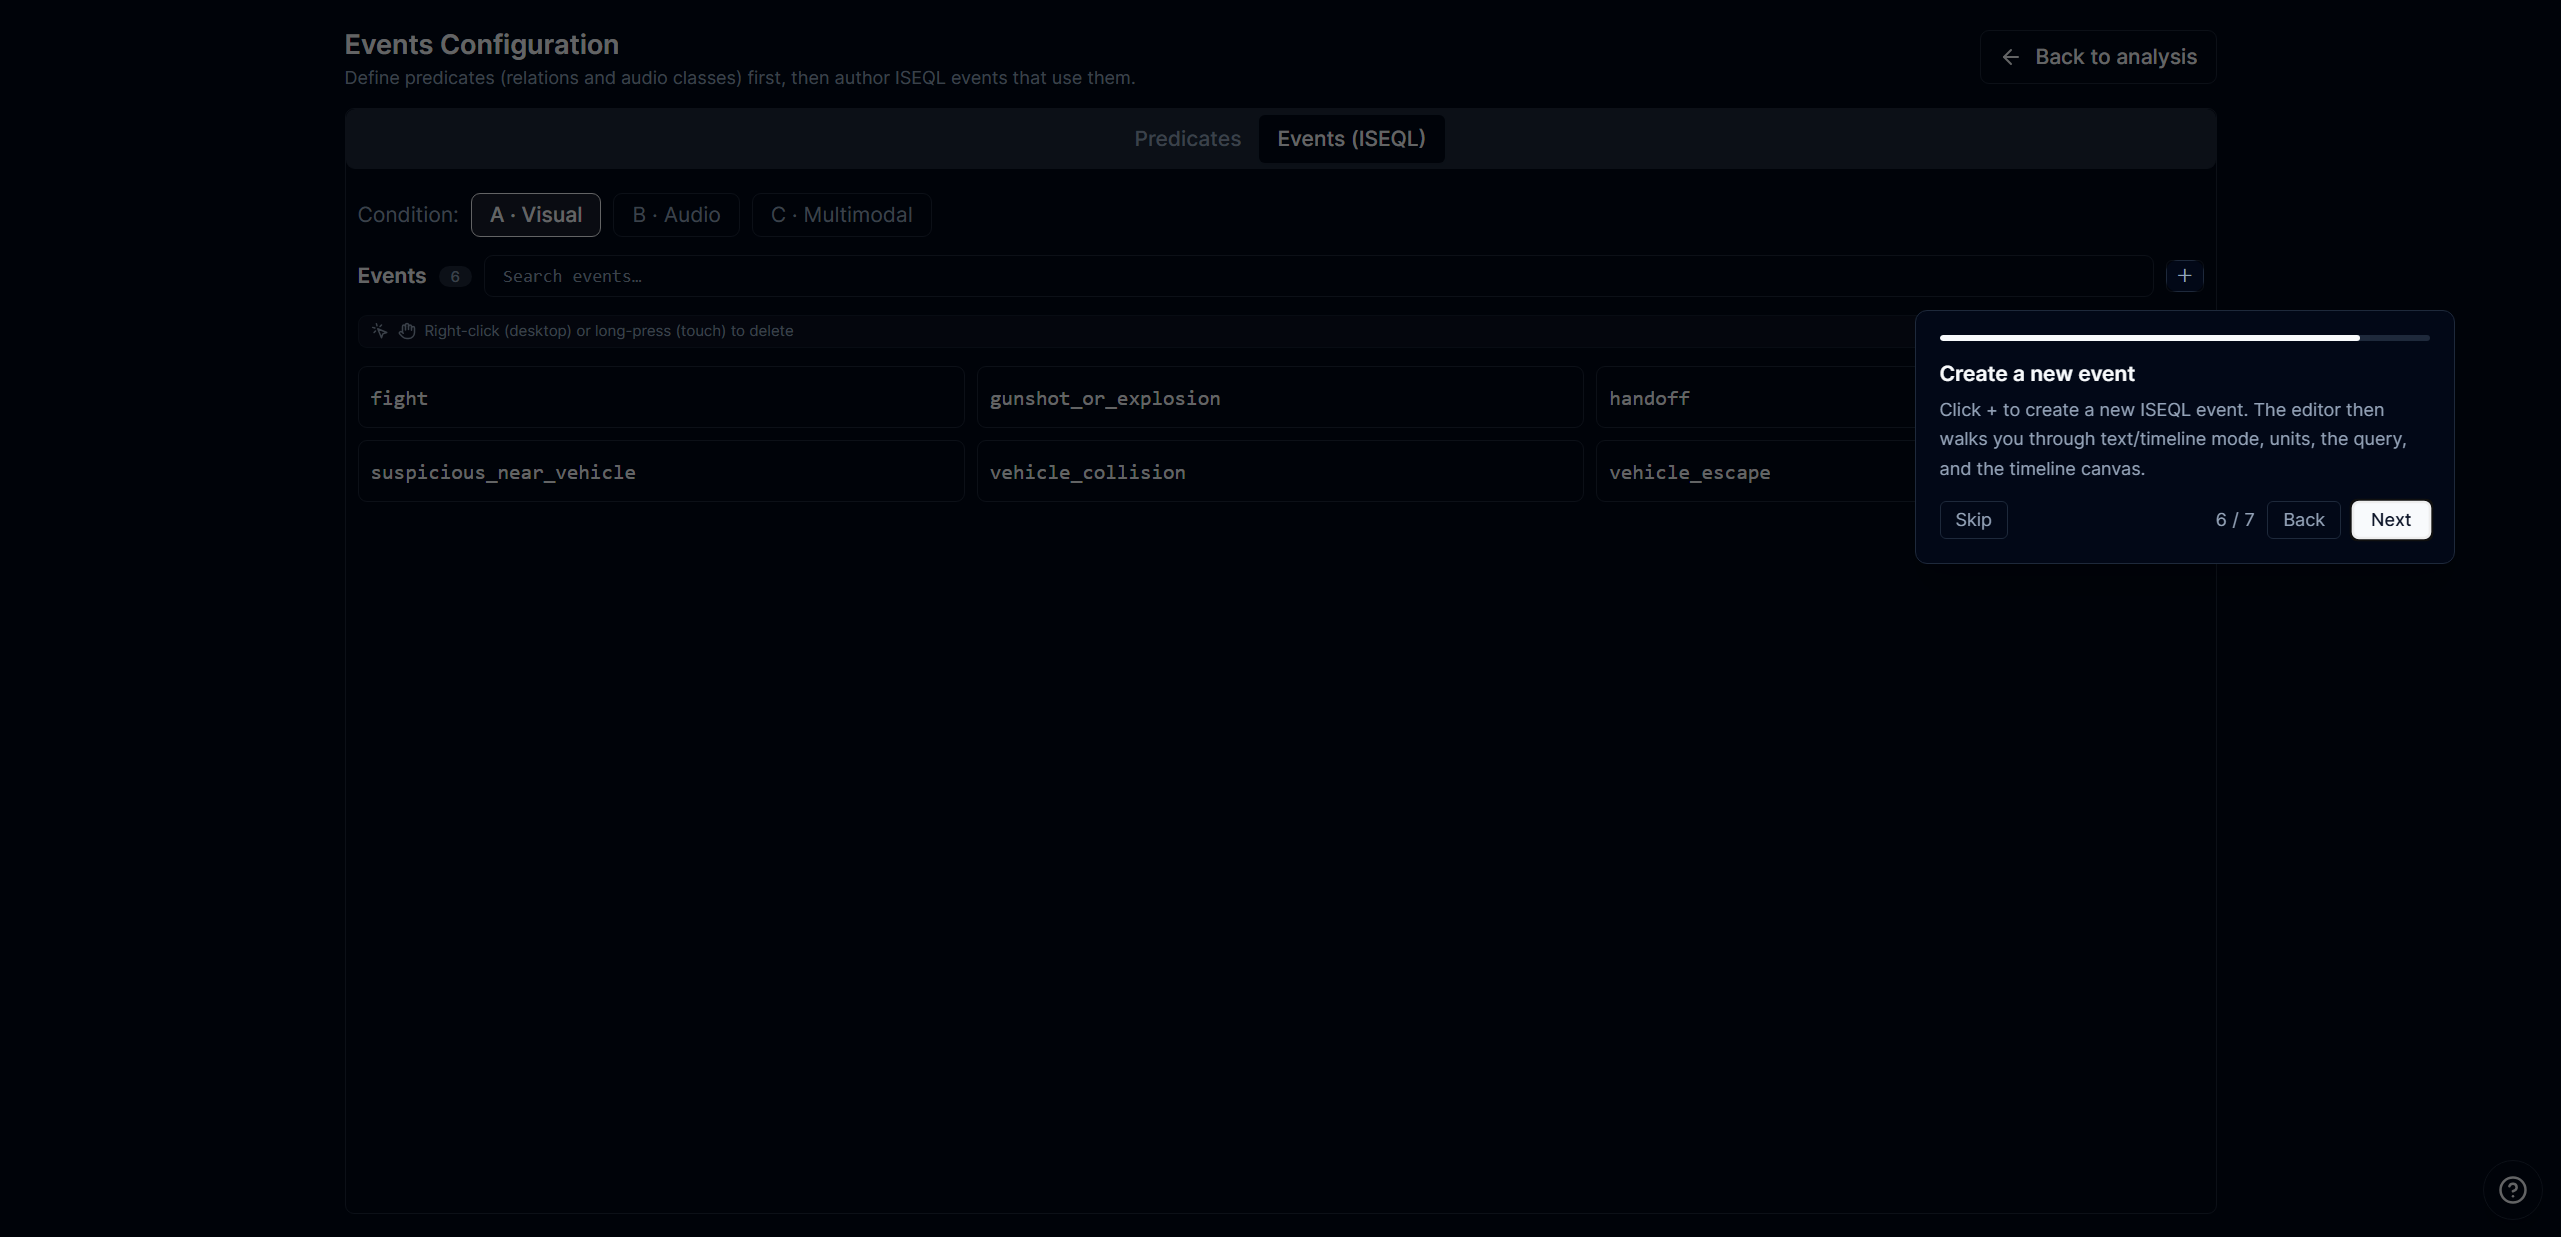
\includegraphics[width=0.92\textwidth]{Figures/appendix/cfg06_events_list.png}
  \caption{Event list: existing events appear here, click to edit.}
\end{figure}

\begin{figure}[H]
  \centering
  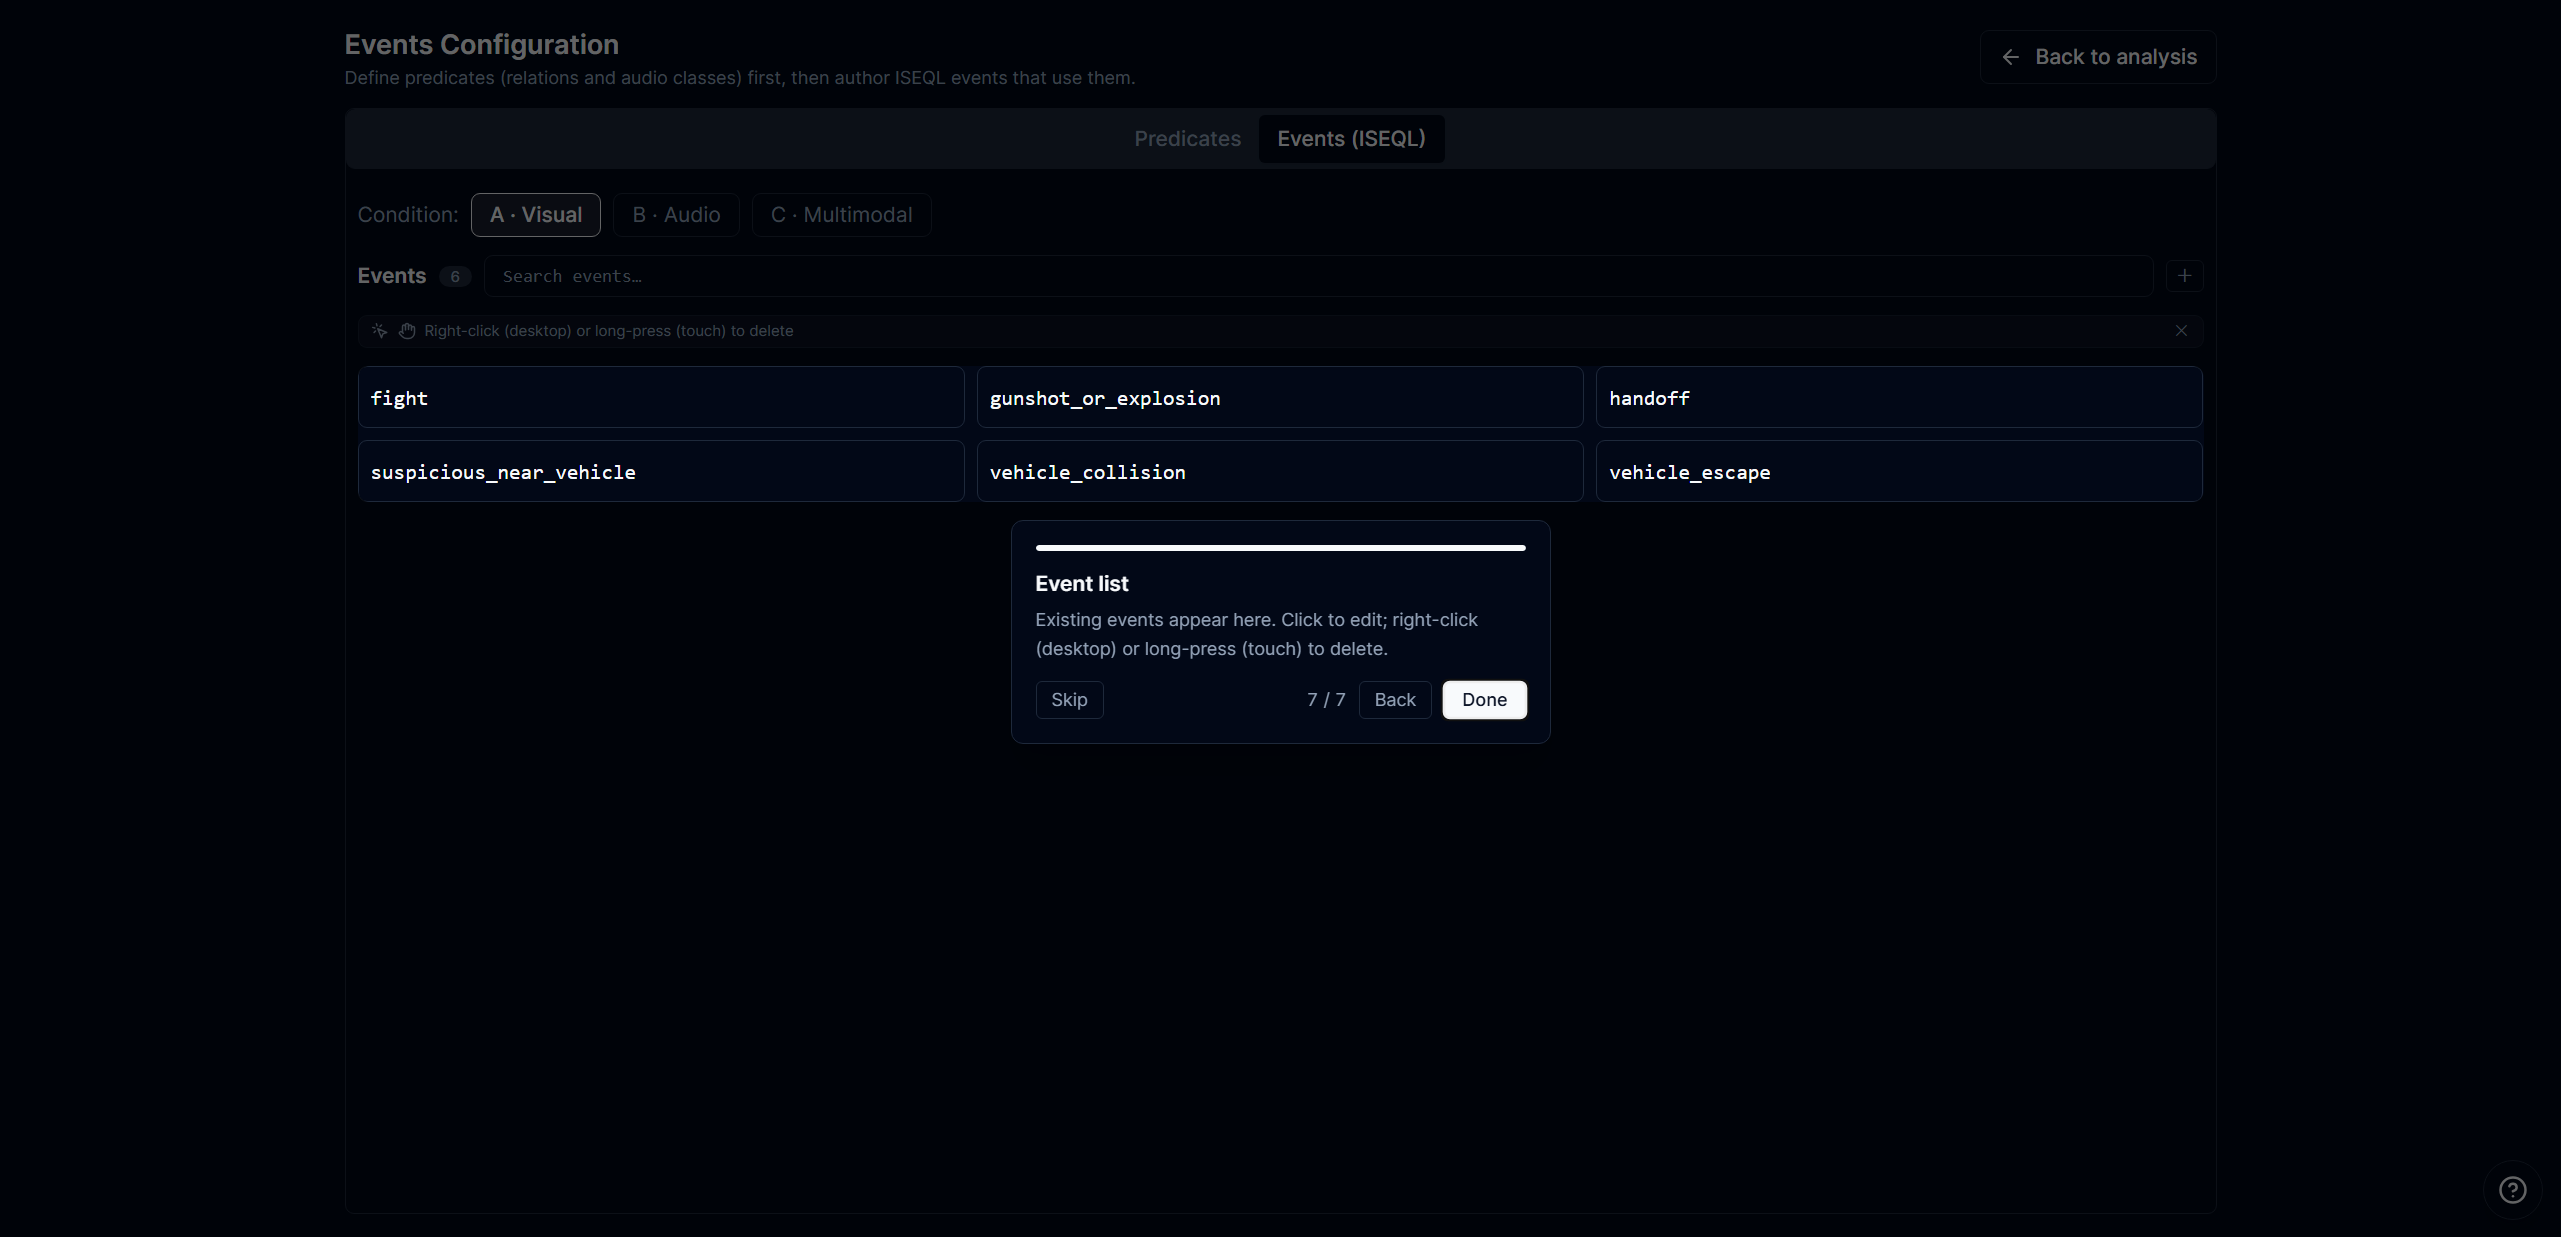
\includegraphics[width=0.92\textwidth]{Figures/appendix/cfg07_event_list_popup.png}
  \caption{Event list: right-click (desktop) or long-press (touch) to delete.}
\end{figure}

\begin{figure}[H]
  \centering
  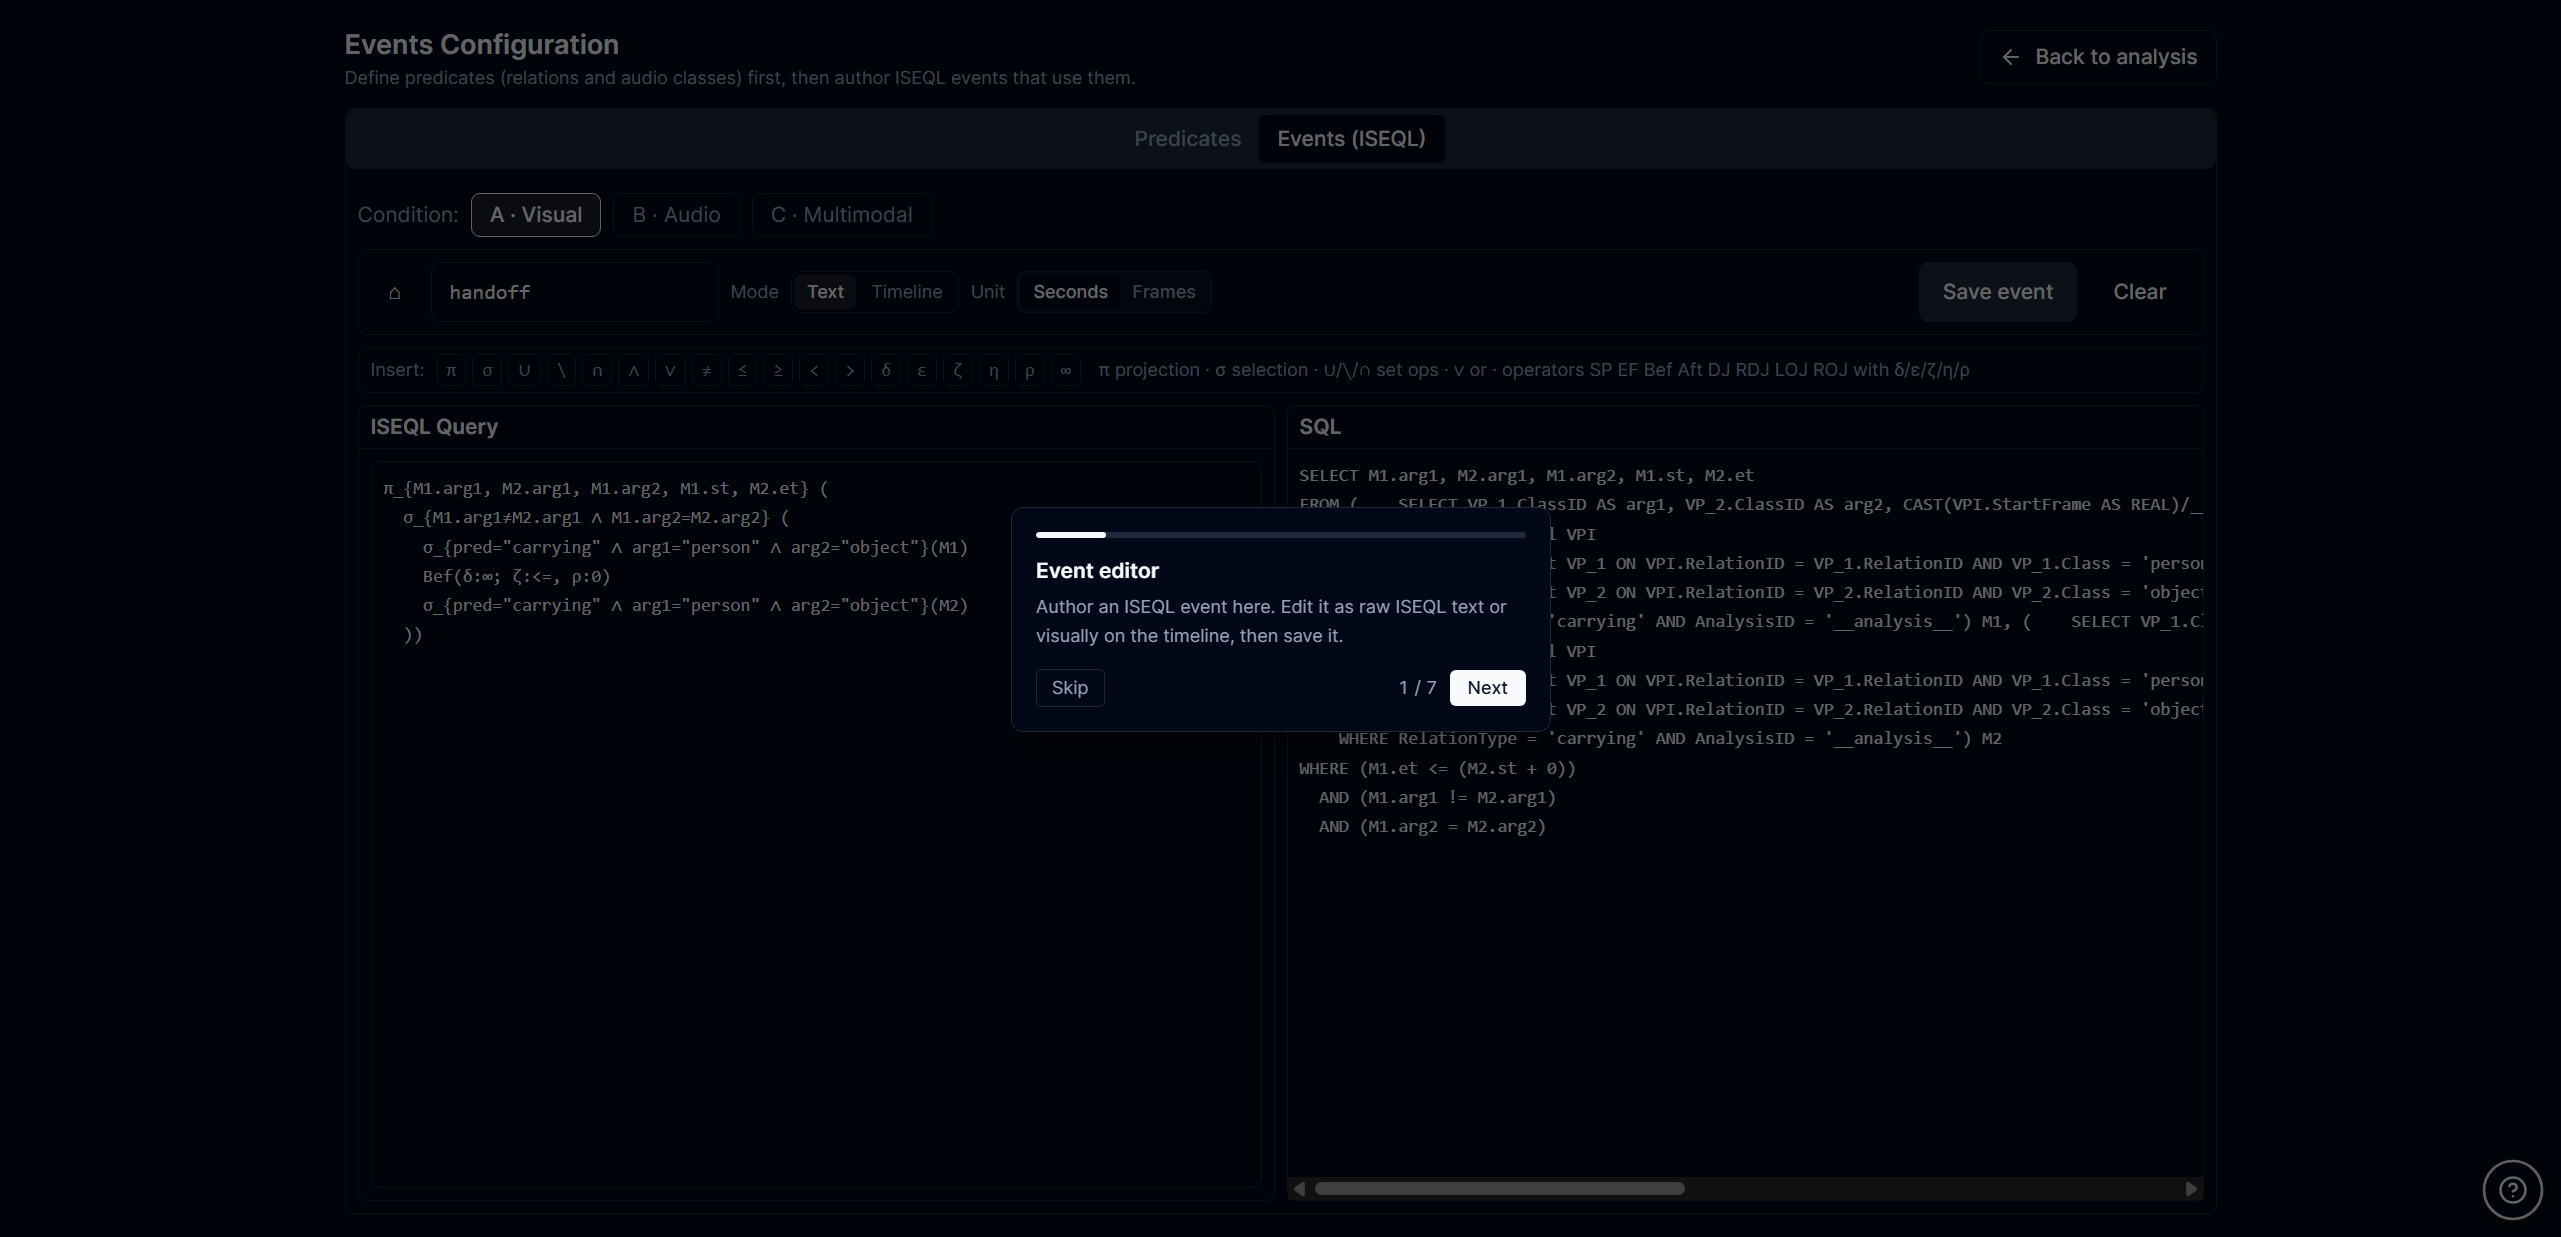
\includegraphics[width=0.92\textwidth]{Figures/appendix/cfg08_editor.png}
  \caption{Event editor: author an ISEQL event as raw text or visually on the timeline.}
\end{figure}

\begin{figure}[H]
  \centering
  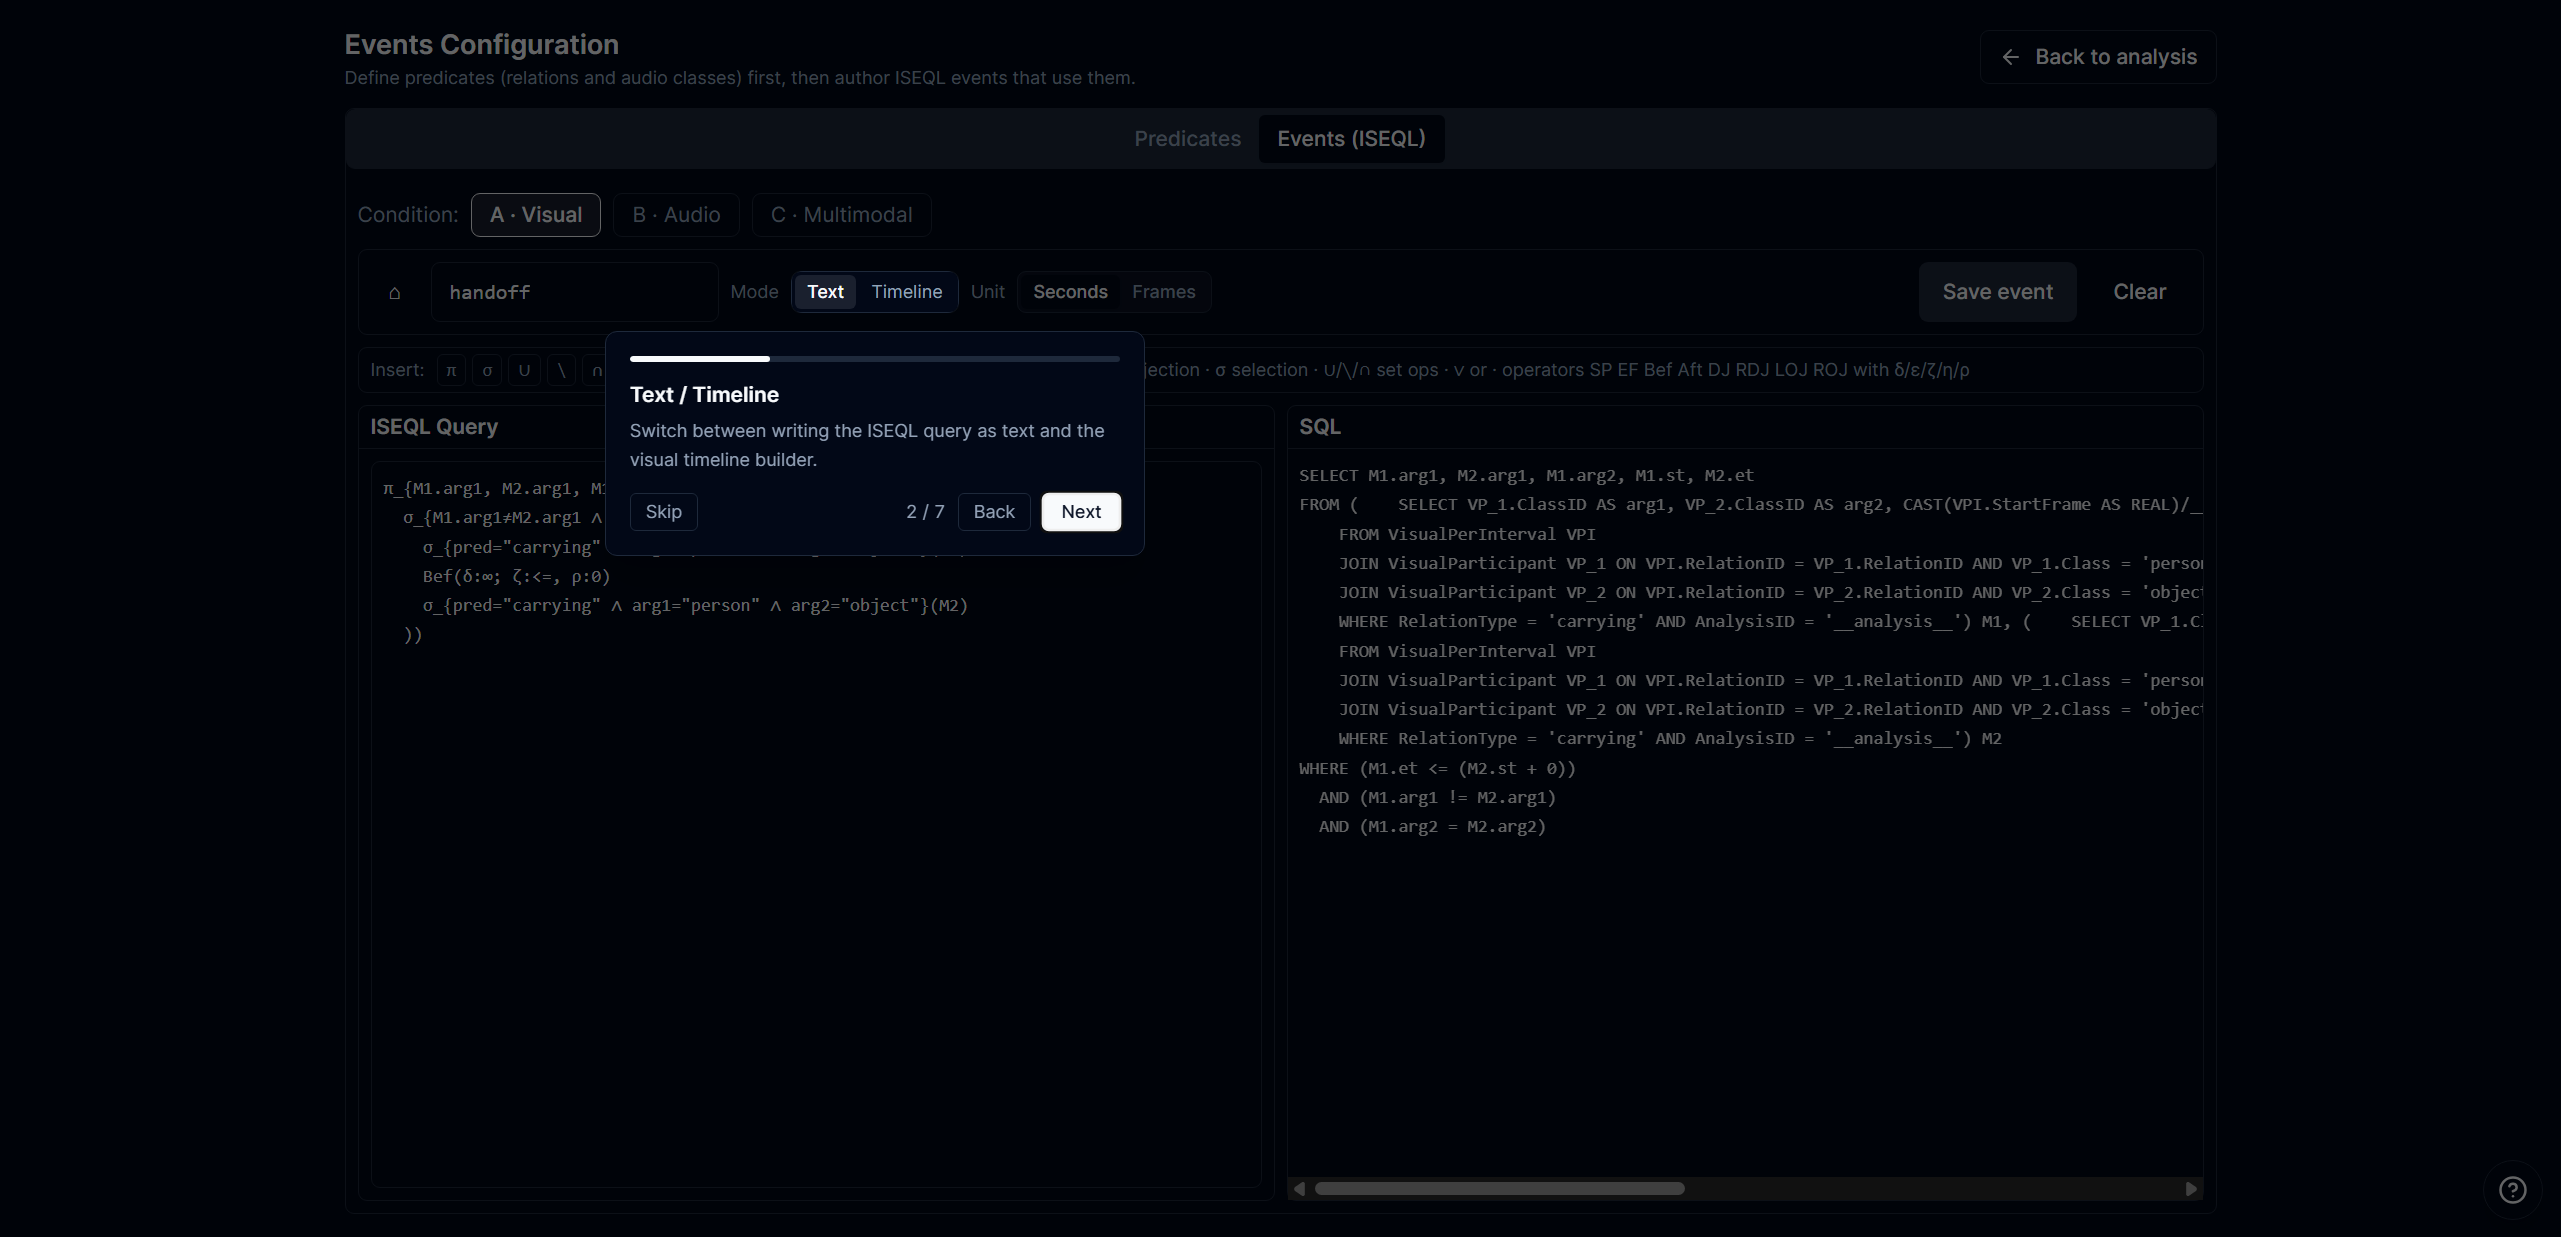
\includegraphics[width=0.92\textwidth]{Figures/appendix/cfg09_mode.png}
  \caption{Text / Timeline: switch between writing the ISEQL query as text and using the visual timeline builder.}
\end{figure}

\begin{figure}[H]
  \centering
  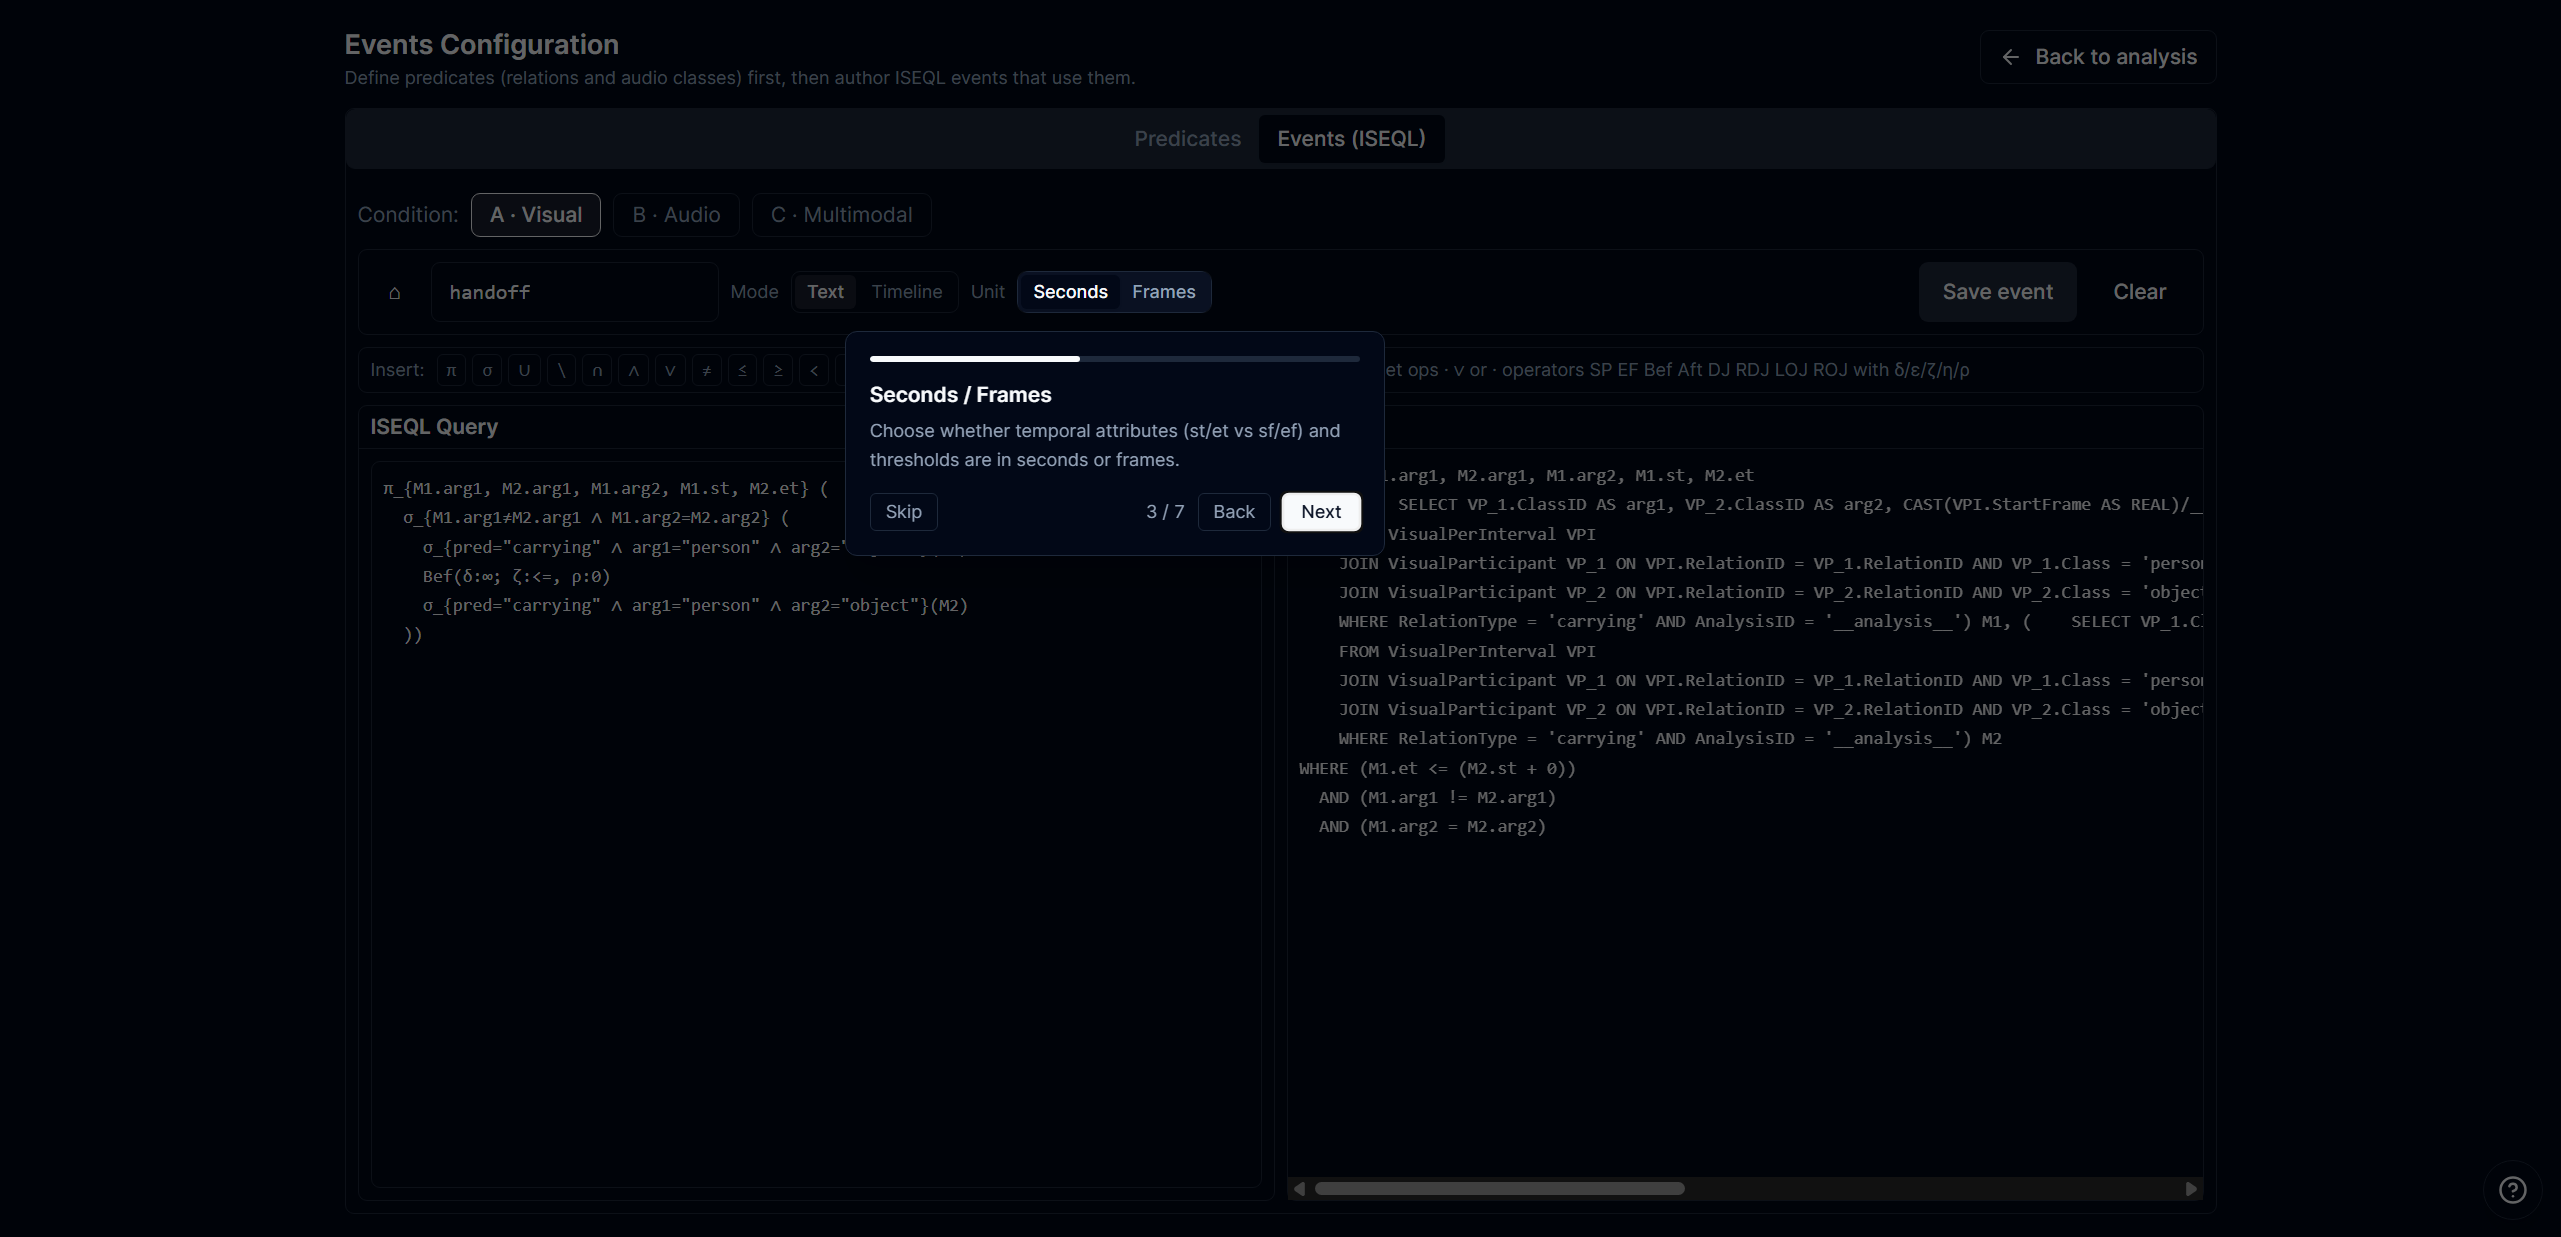
\includegraphics[width=0.92\textwidth]{Figures/appendix/cfg10_units.png}
  \caption{Seconds / Frames: choose whether temporal attributes (st/et vs sf/ef) are in seconds or frames.}
\end{figure}

\begin{figure}[H]
  \centering
  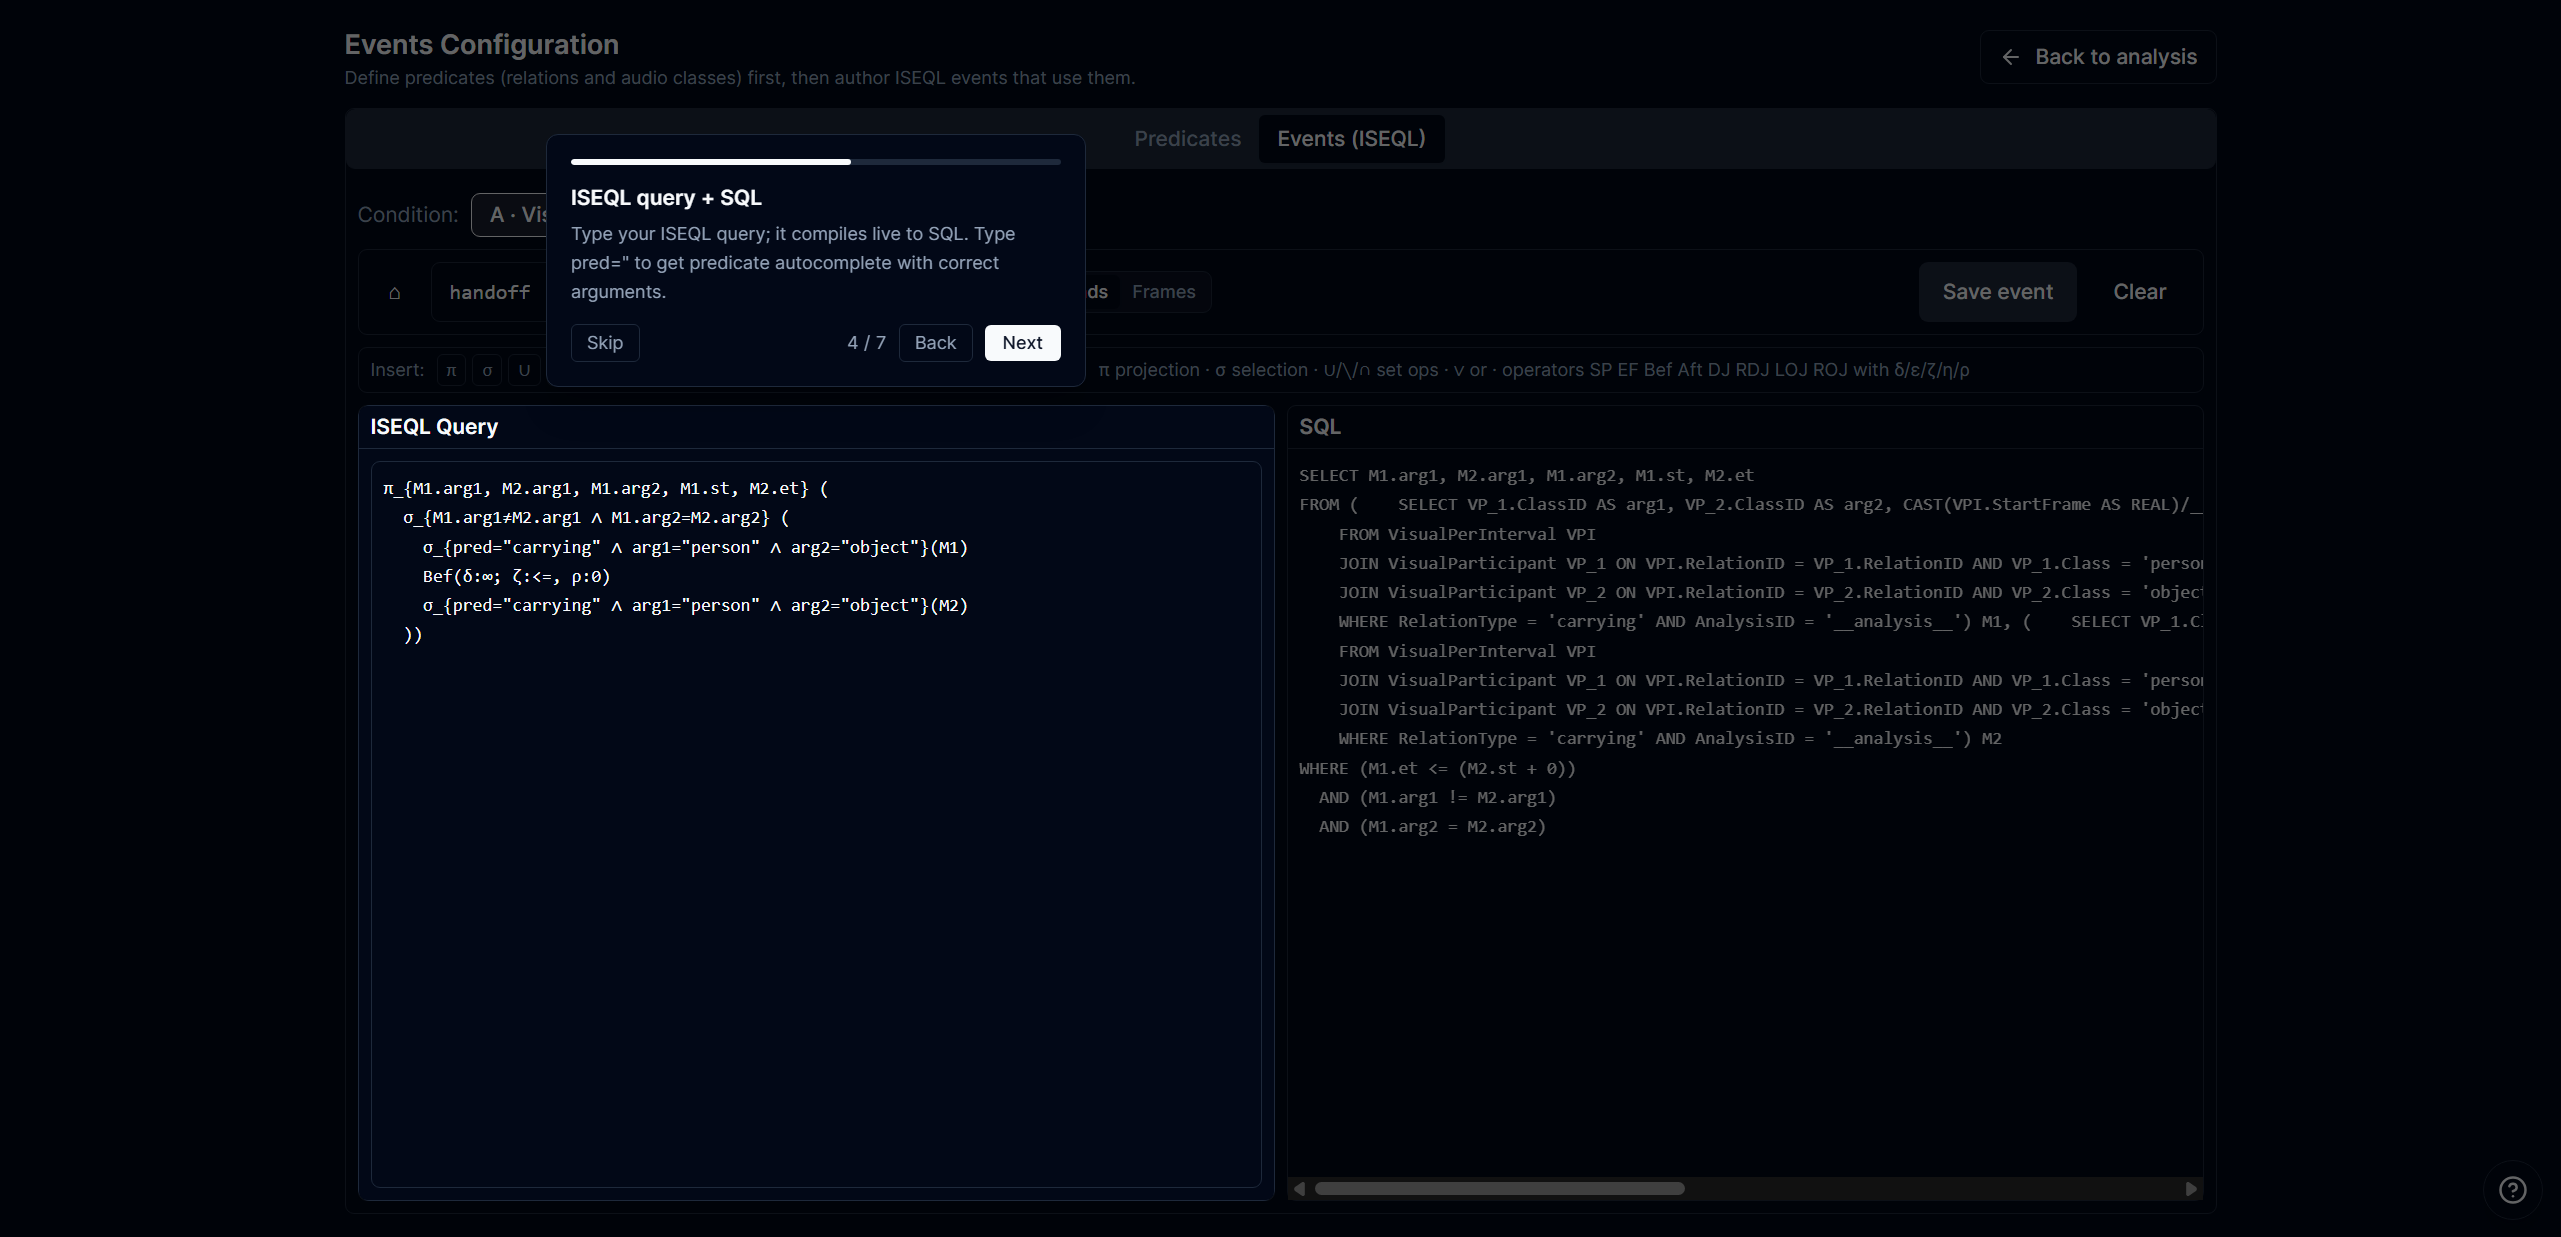
\includegraphics[width=0.92\textwidth]{Figures/appendix/cfg11_query_sql.png}
  \caption{ISEQL query + SQL: type the ISEQL query; it compiles live to SQL.}
\end{figure}

\begin{figure}[H]
  \centering
  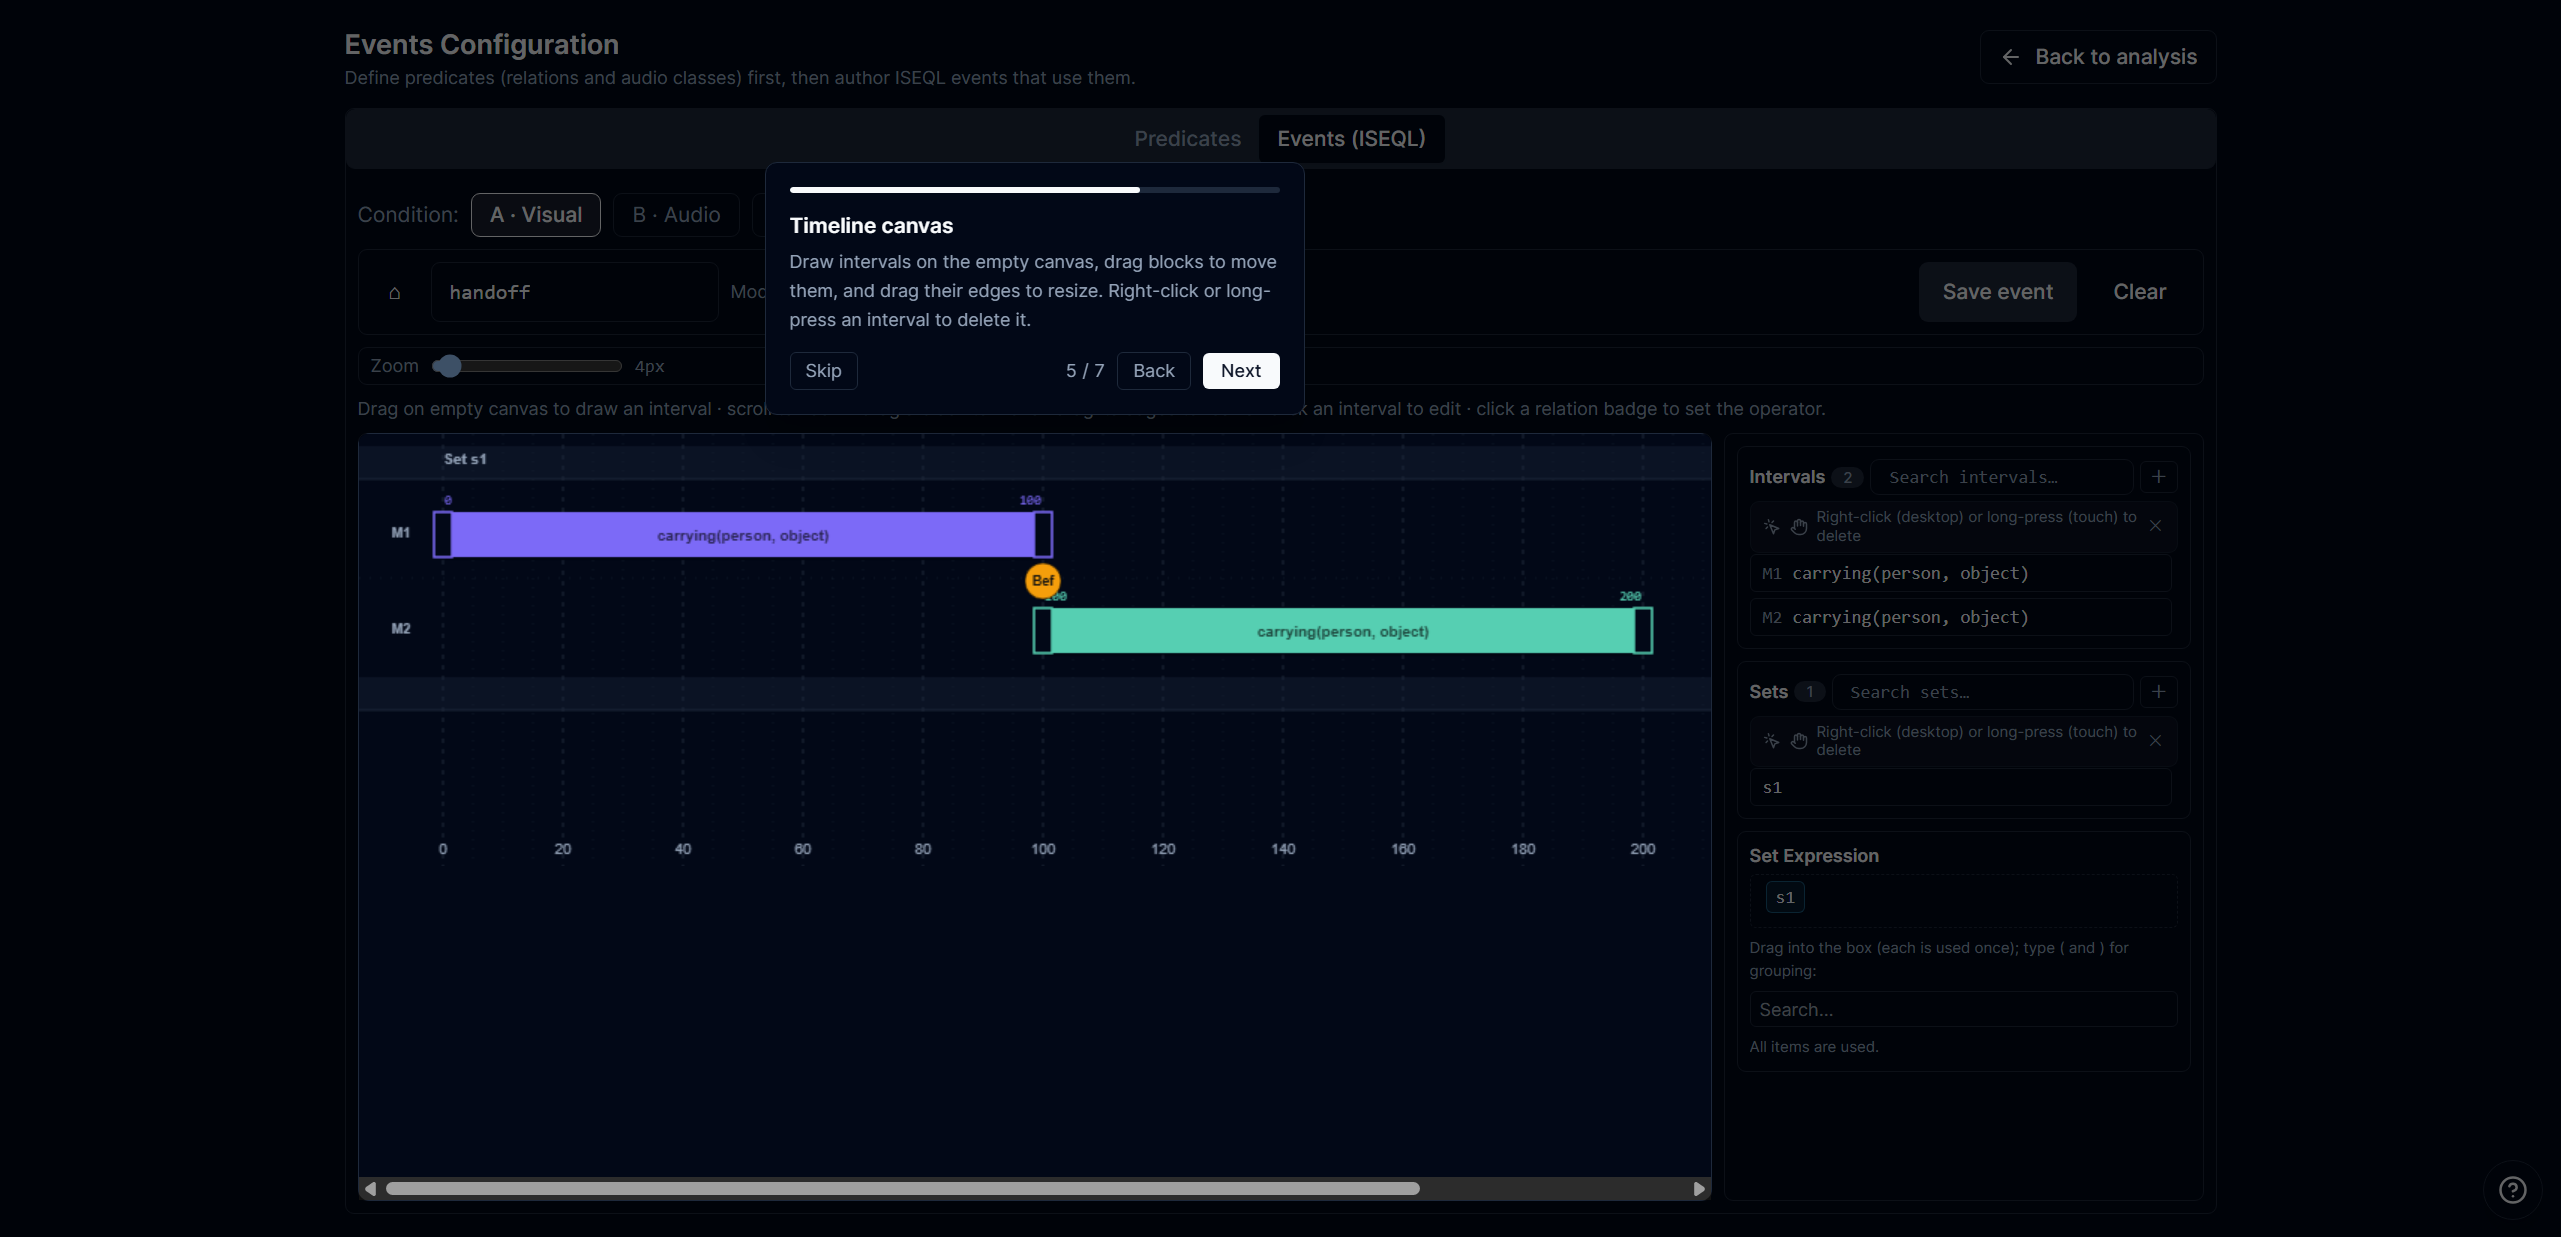
\includegraphics[width=0.92\textwidth]{Figures/appendix/cfg12_timeline.png}
  \caption{Timeline canvas: draw intervals, drag blocks to move them, and drag their edges to resize.}
\end{figure}

\begin{figure}[H]
  \centering
  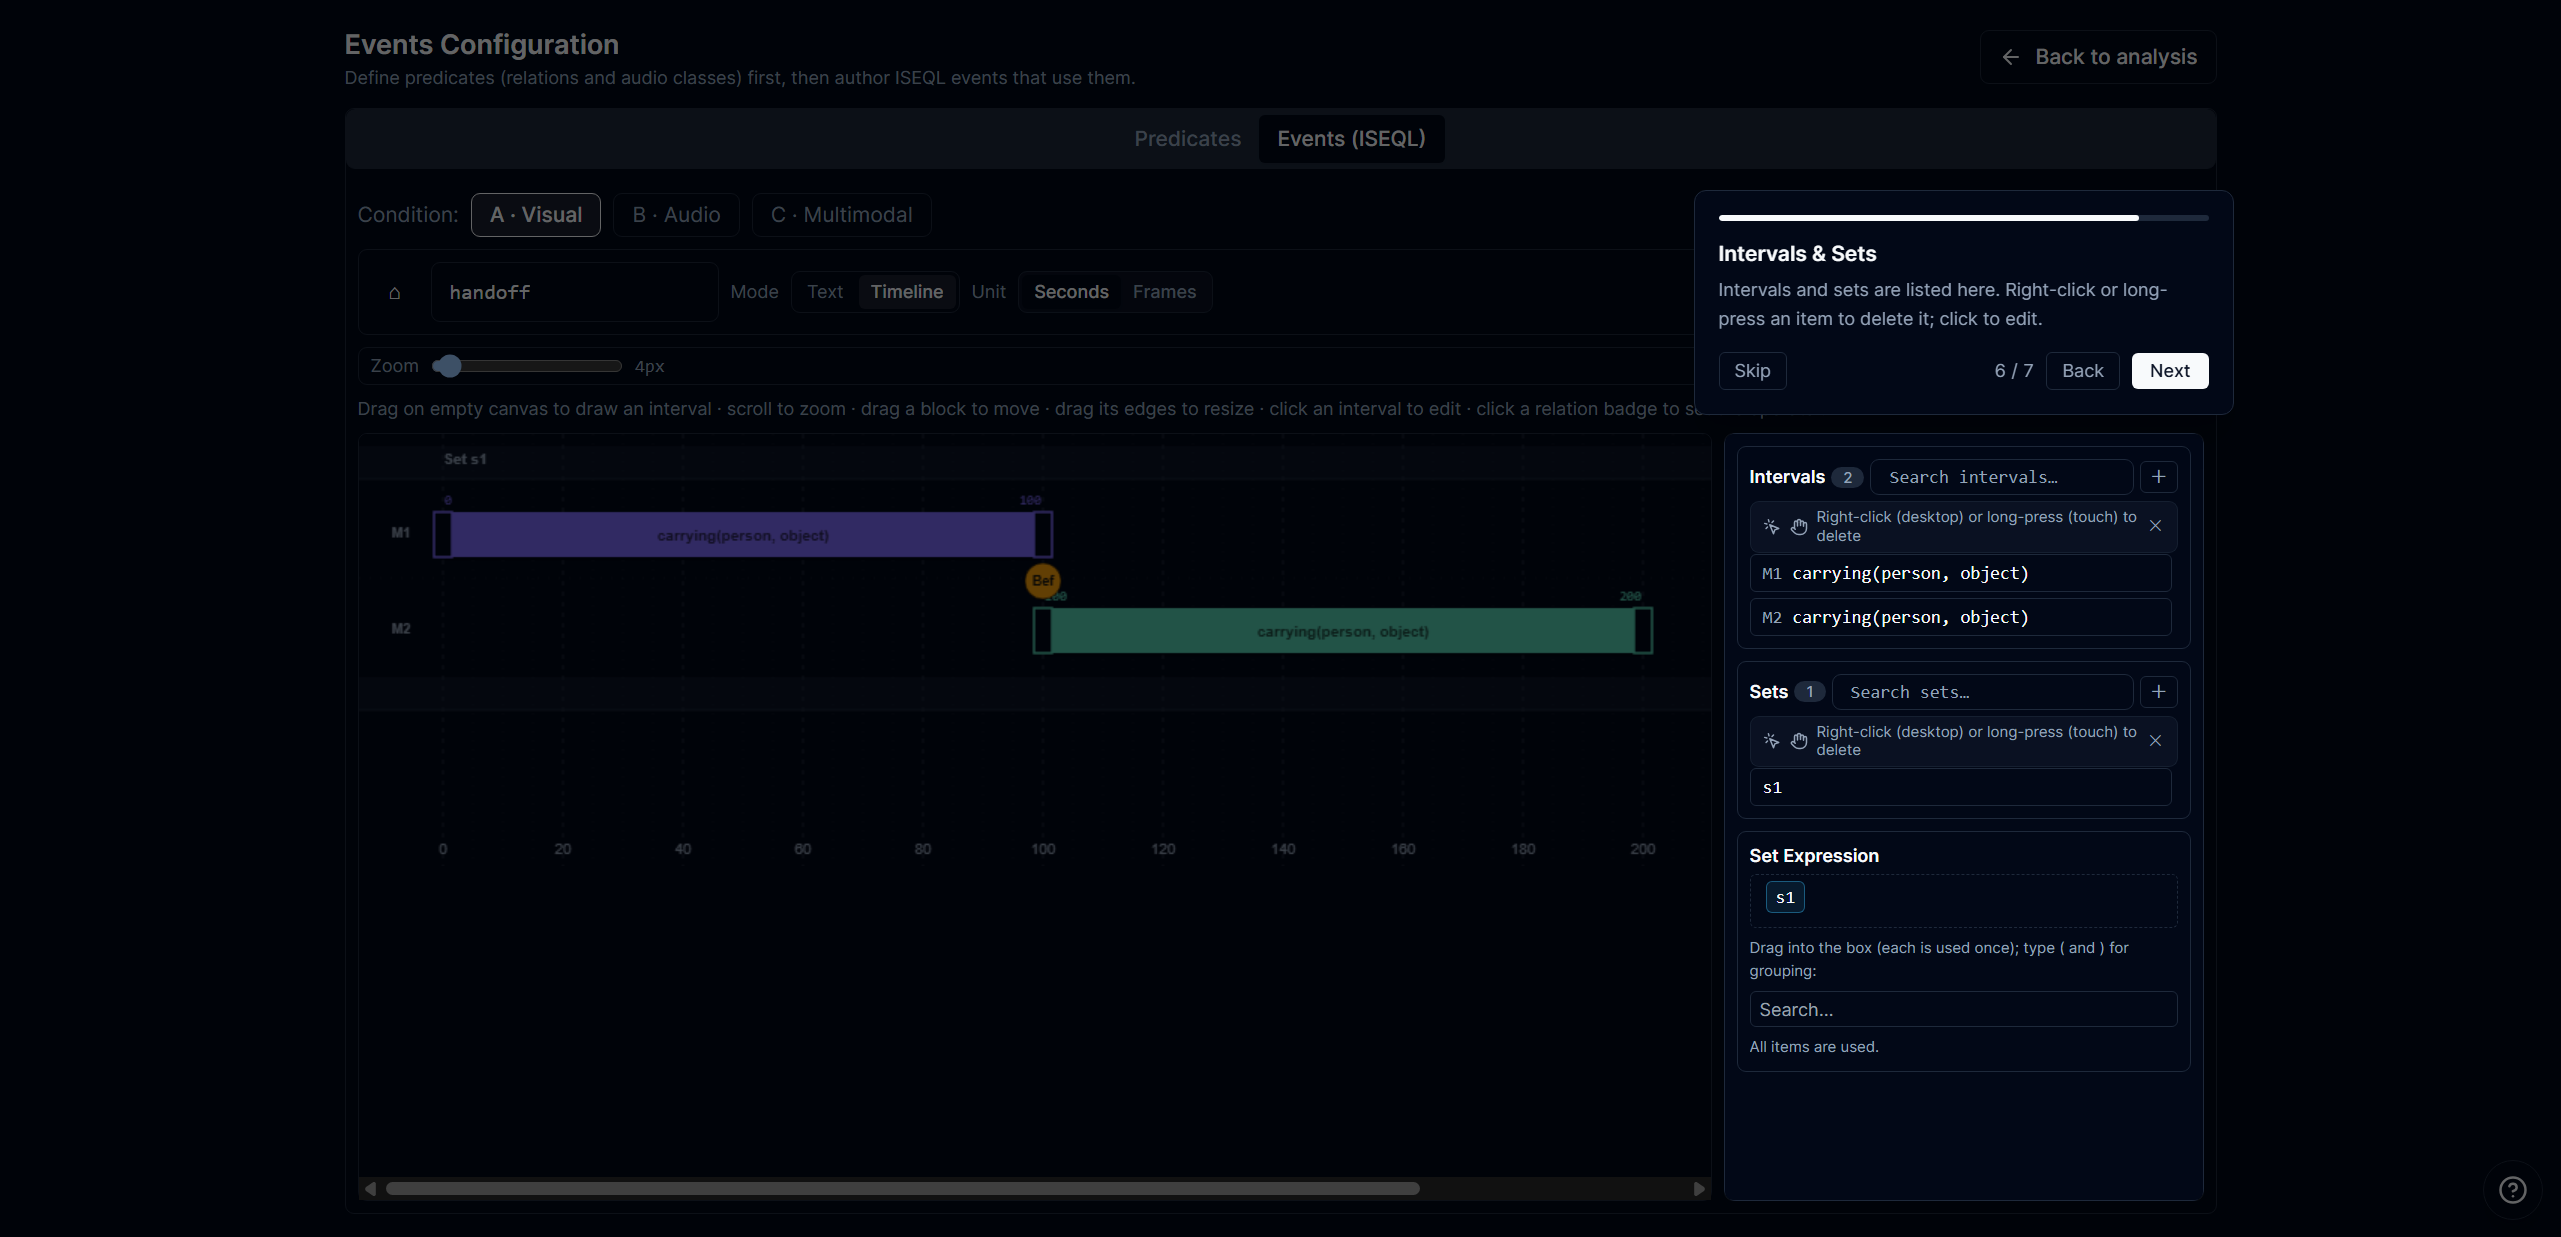
\includegraphics[width=0.92\textwidth]{Figures/appendix/cfg13_timeline_clean.png}
  \caption{Intervals and sets: intervals and sets are listed here; click an item to edit.}
\end{figure}

\begin{figure}[H]
  \centering
  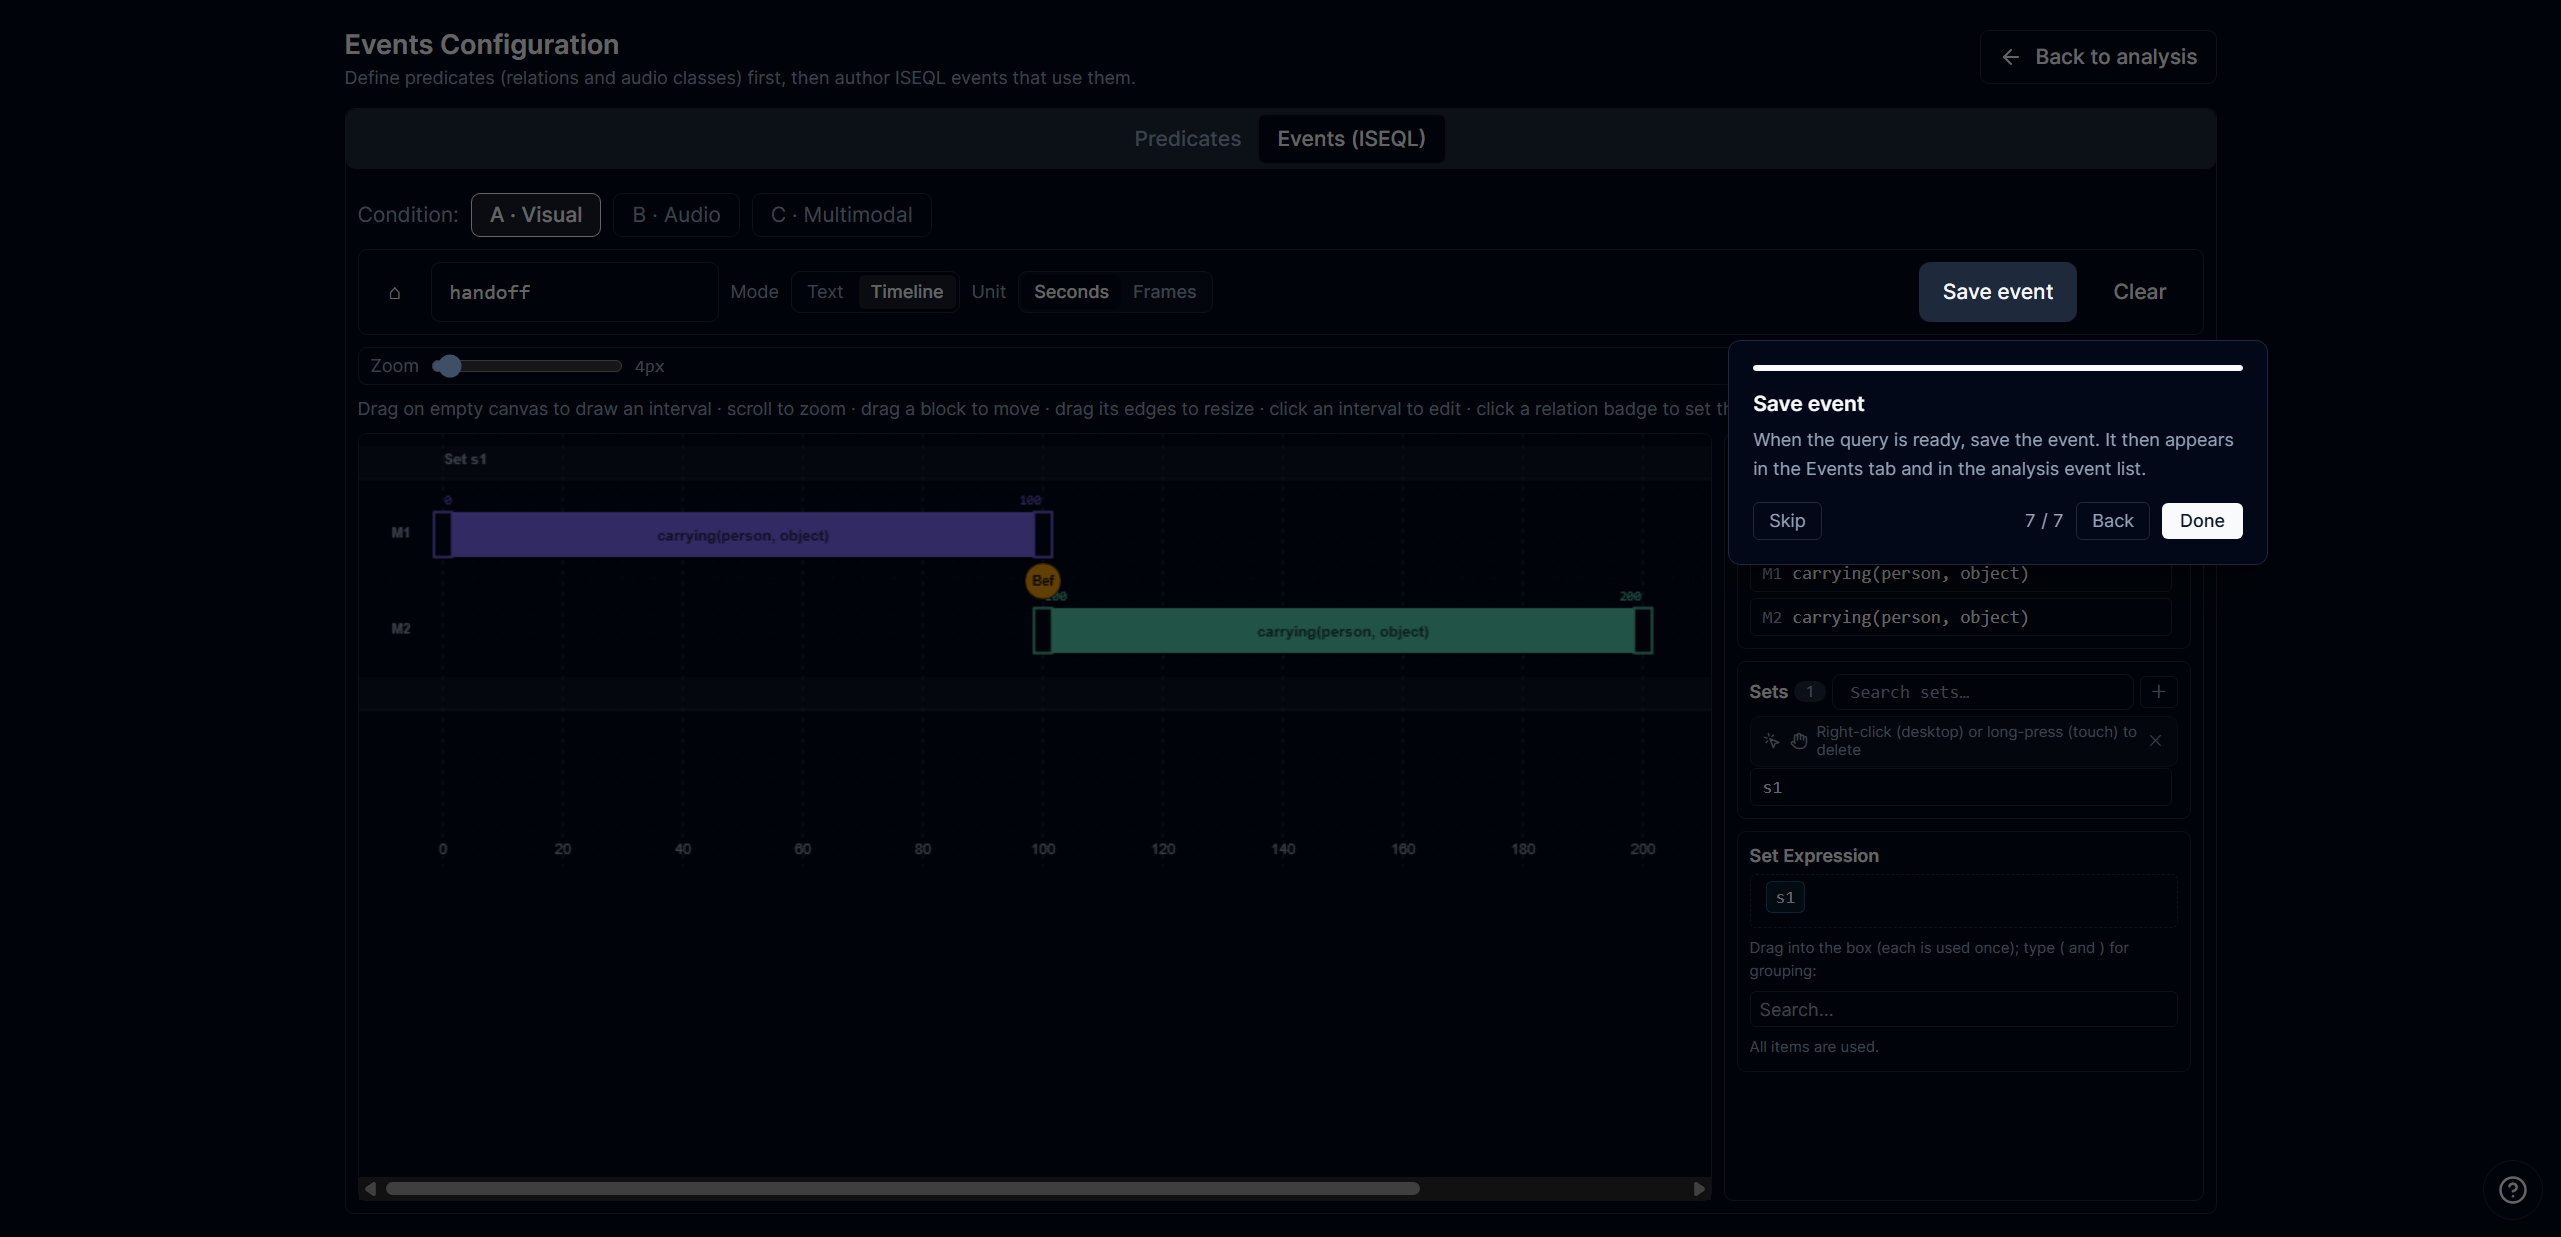
\includegraphics[width=0.92\textwidth]{Figures/appendix/cfg14_timeline_save.png}
  \caption{Save event: when the query is ready, save the event.}
\end{figure}

\section{Visual Only: Handoff}

This example runs condition A (visual only) with the Gemini 3.6 Flash VLM and object re-identification to detect the handoff event. The following figures show the analysis page and the object memory used to maintain consistent object identities.

\begin{figure}[H]
  \centering
  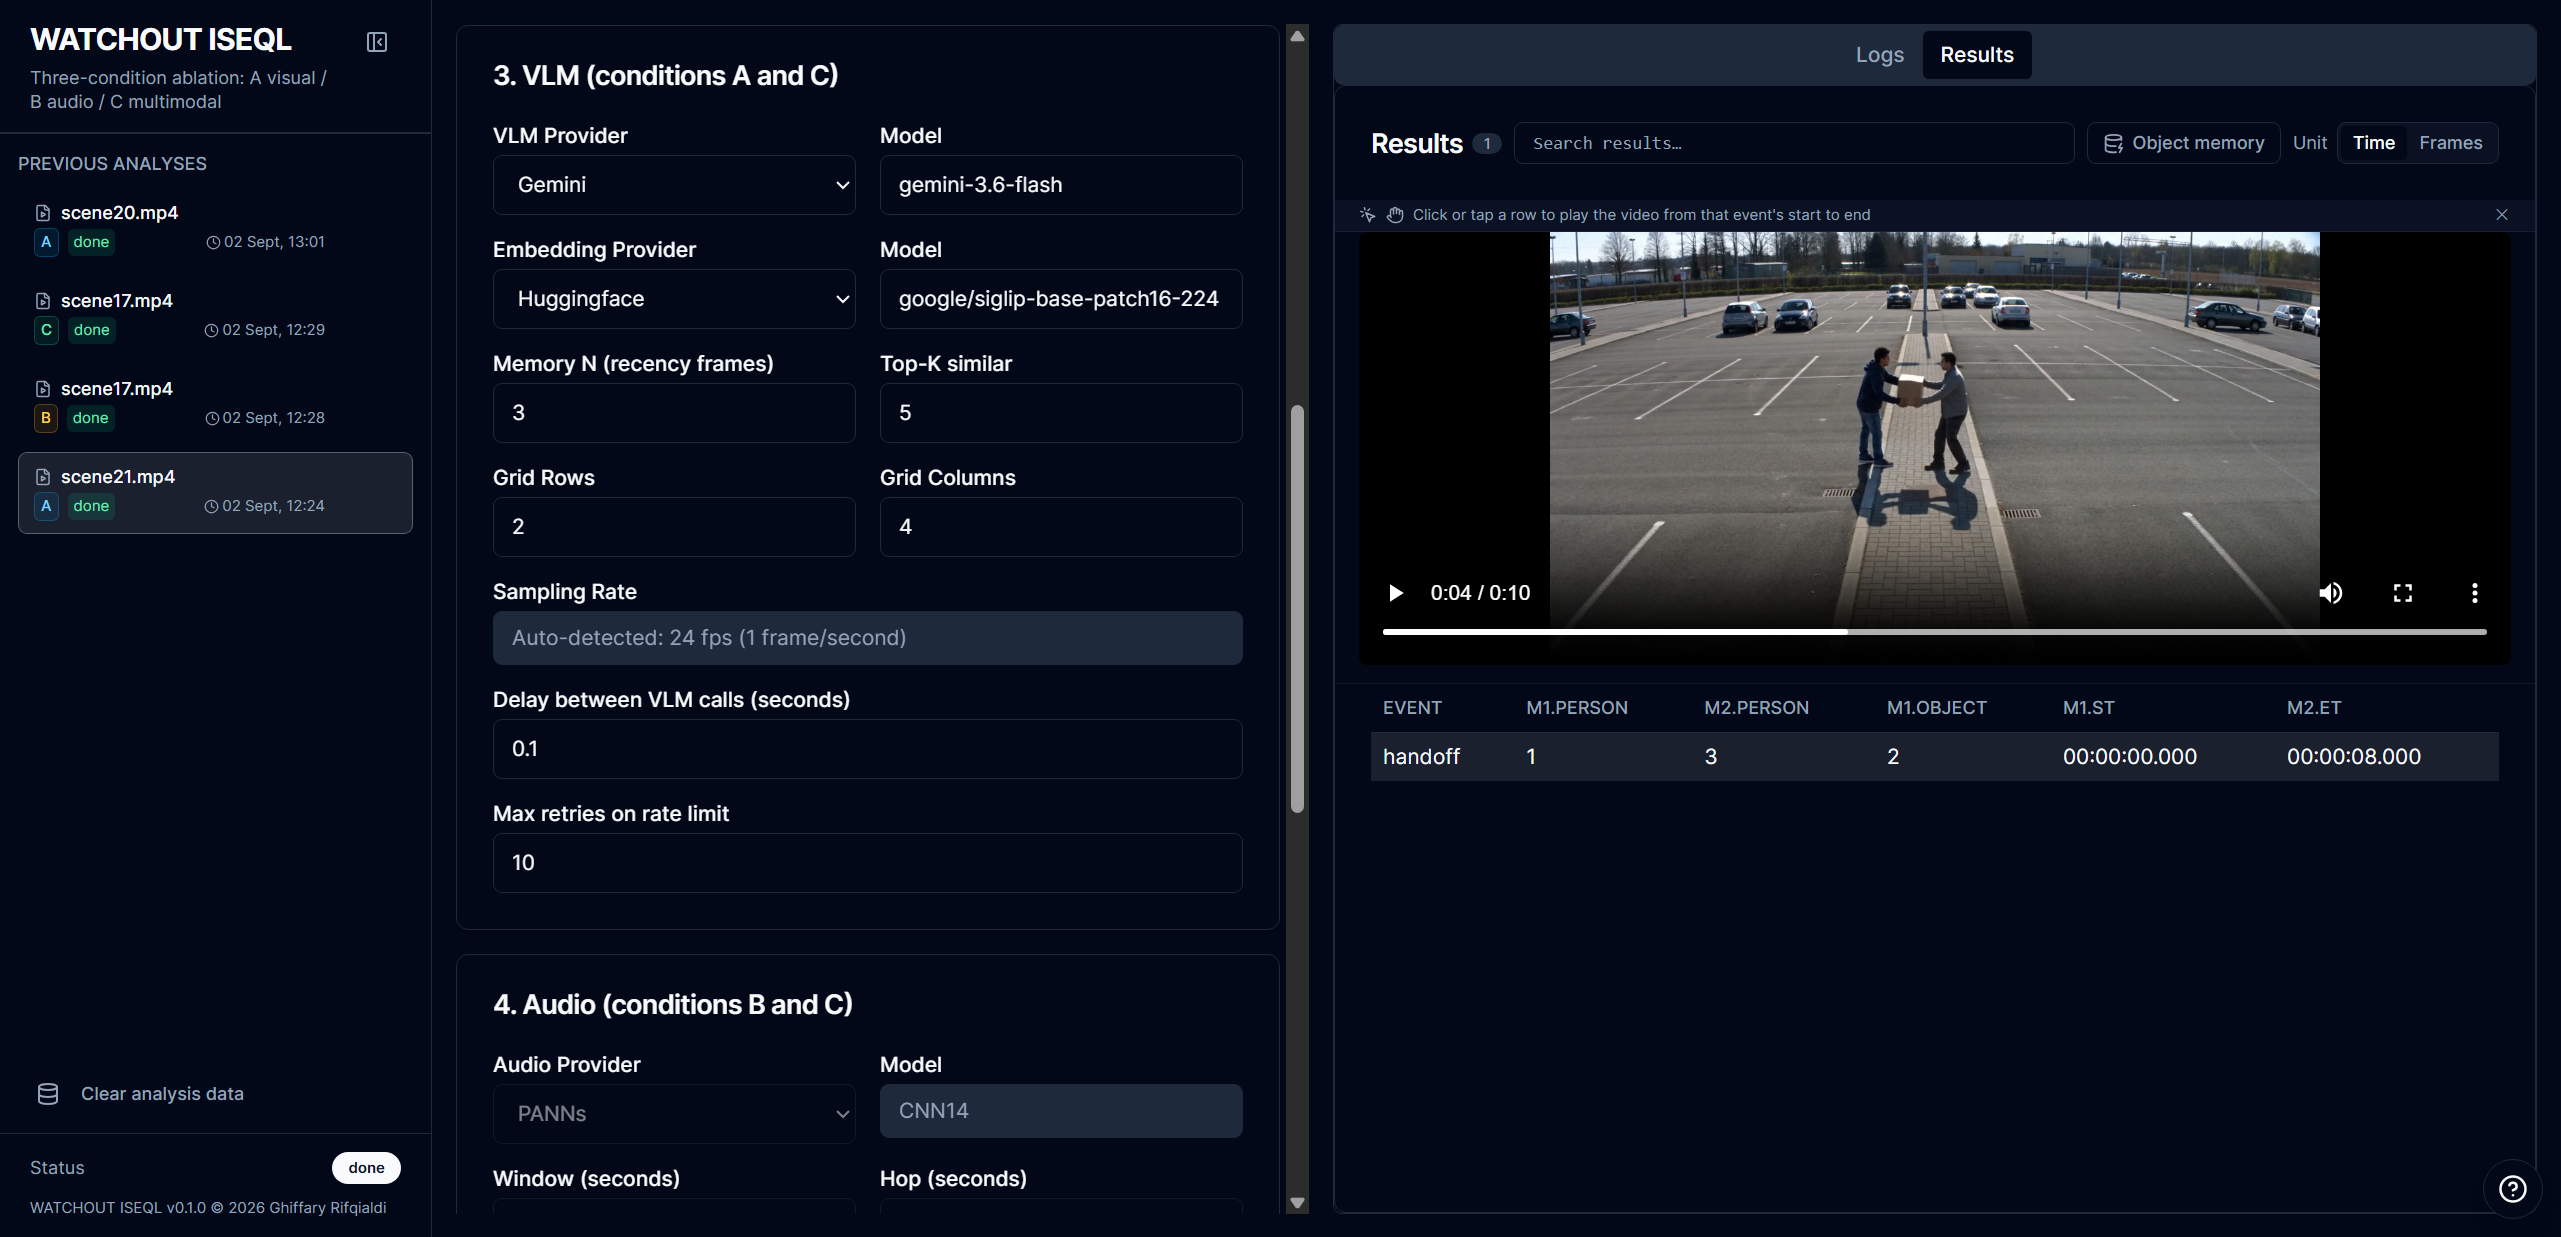
\includegraphics[width=0.92\textwidth]{Figures/appendix/va01_results.png}
  \caption{Visual only (handoff): the results report a handoff detection. The M1.PERSON, M2.PERSON and M1.OBJECT columns hold the persistent identities assigned by re-identification, so the exact people and object involved can be identified.}
\end{figure}

\begin{figure}[H]
  \centering
  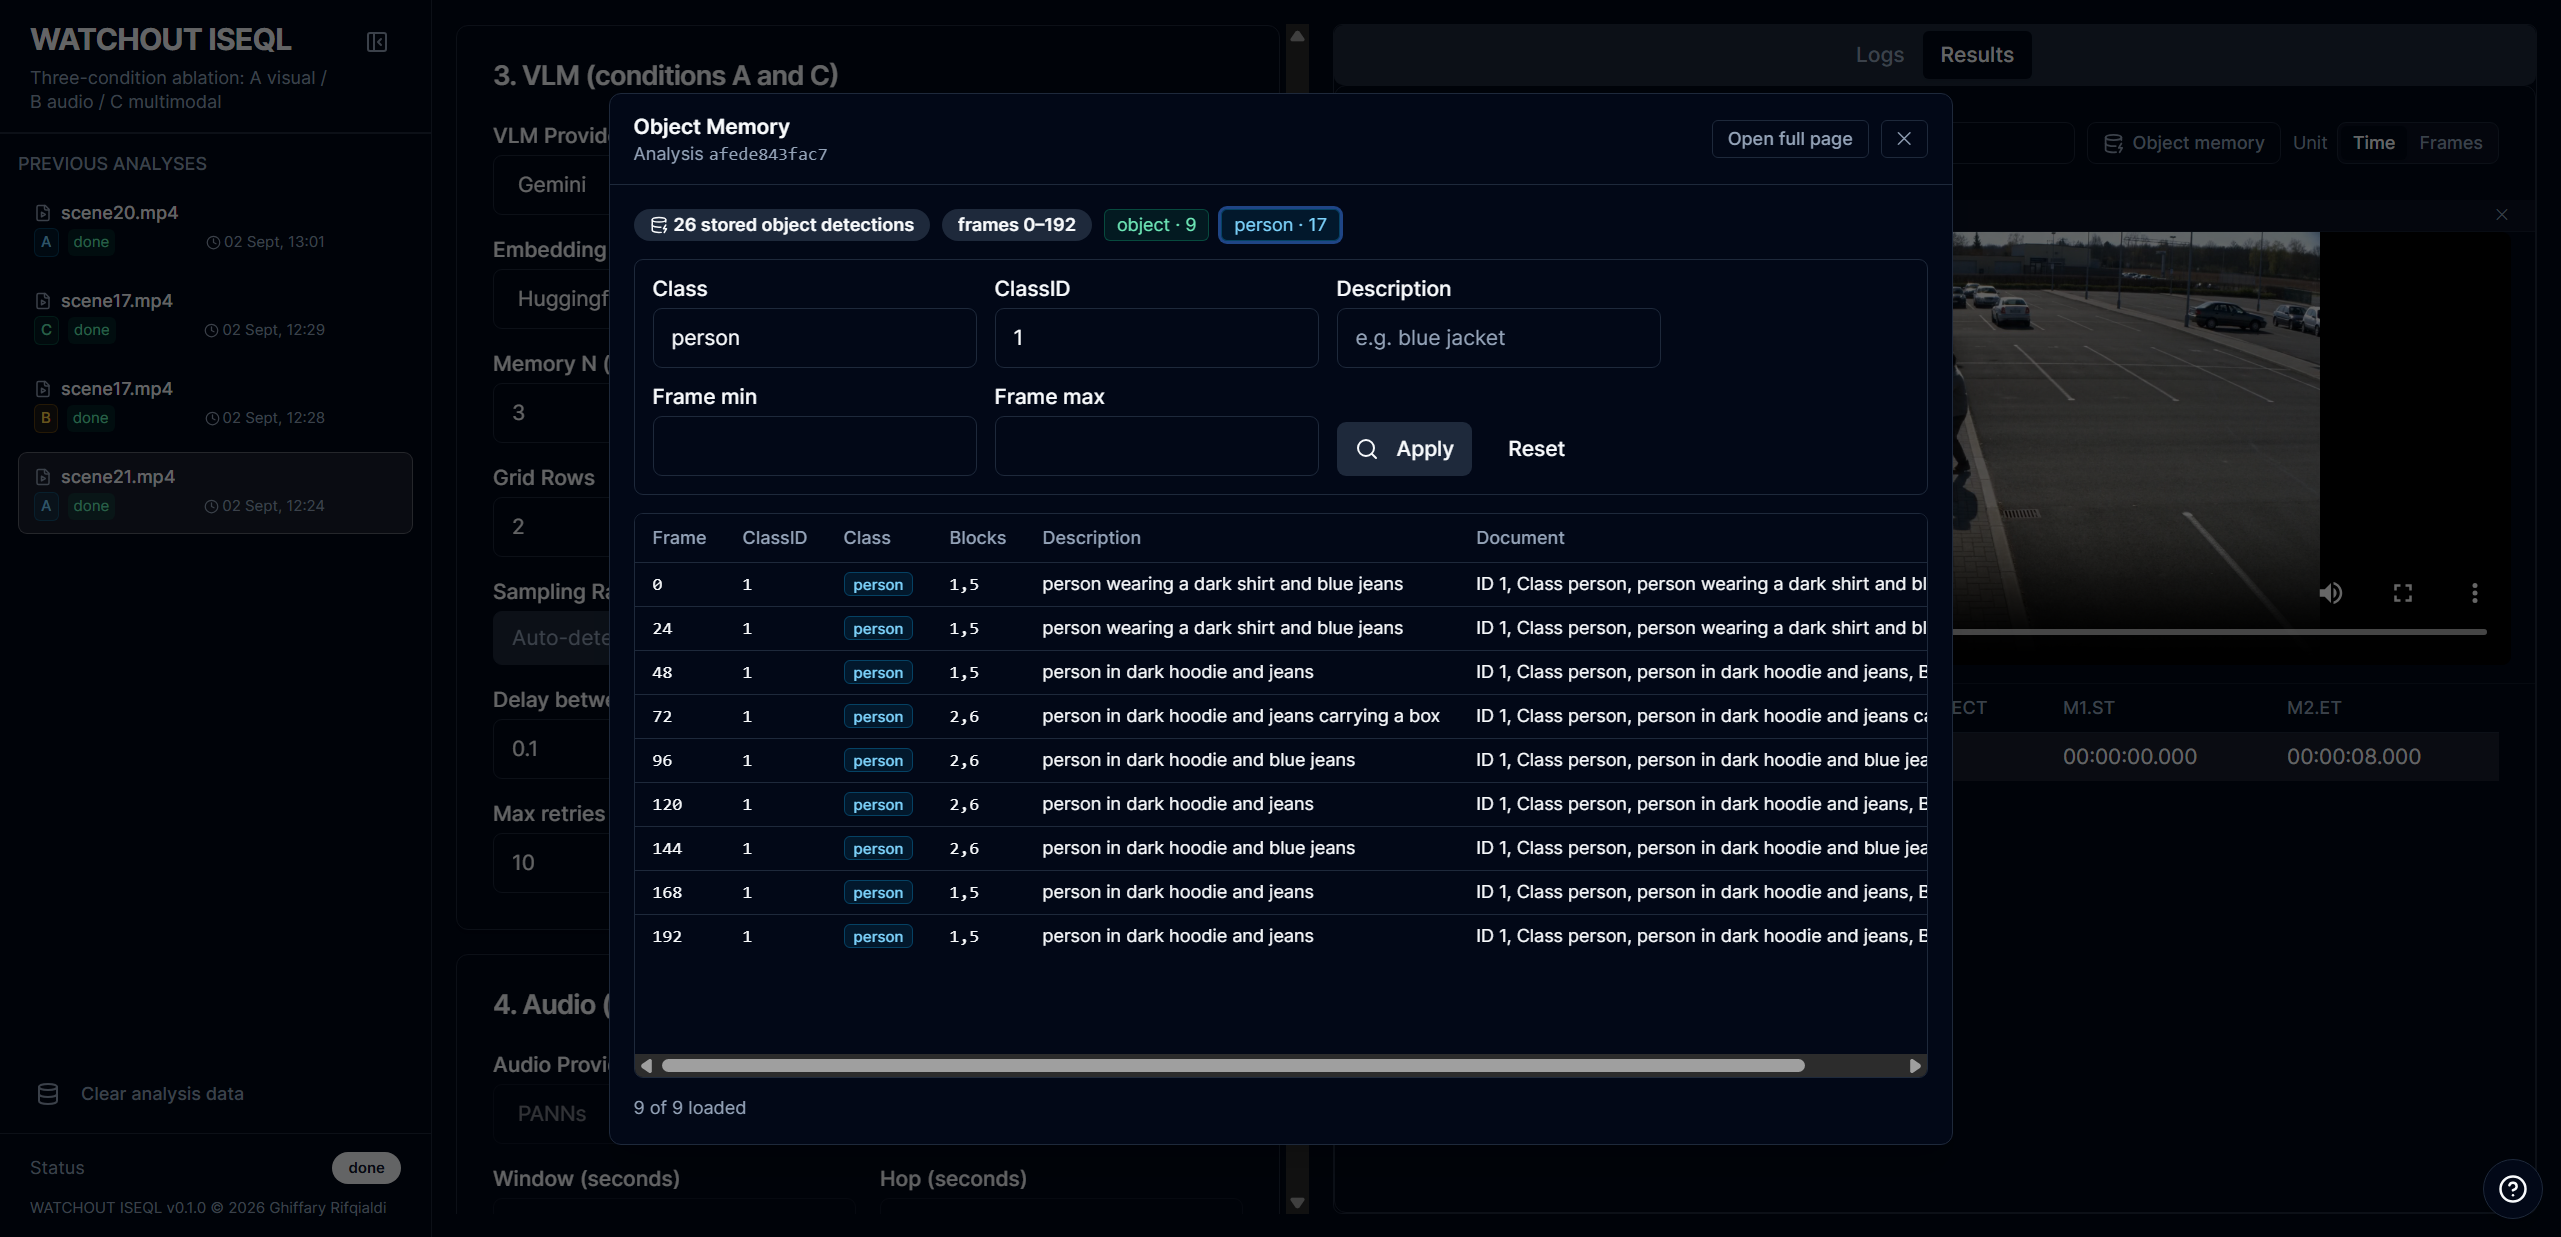
\includegraphics[width=0.92\textwidth]{Figures/appendix/va02_memory_person1.png}
  \caption{Object Memory (visual only, handoff example): person identity 1 (dark shirt); the M1.PERSON column in the result points to this identity, so the person is traceable across the video.}
\end{figure}

\begin{figure}[H]
  \centering
  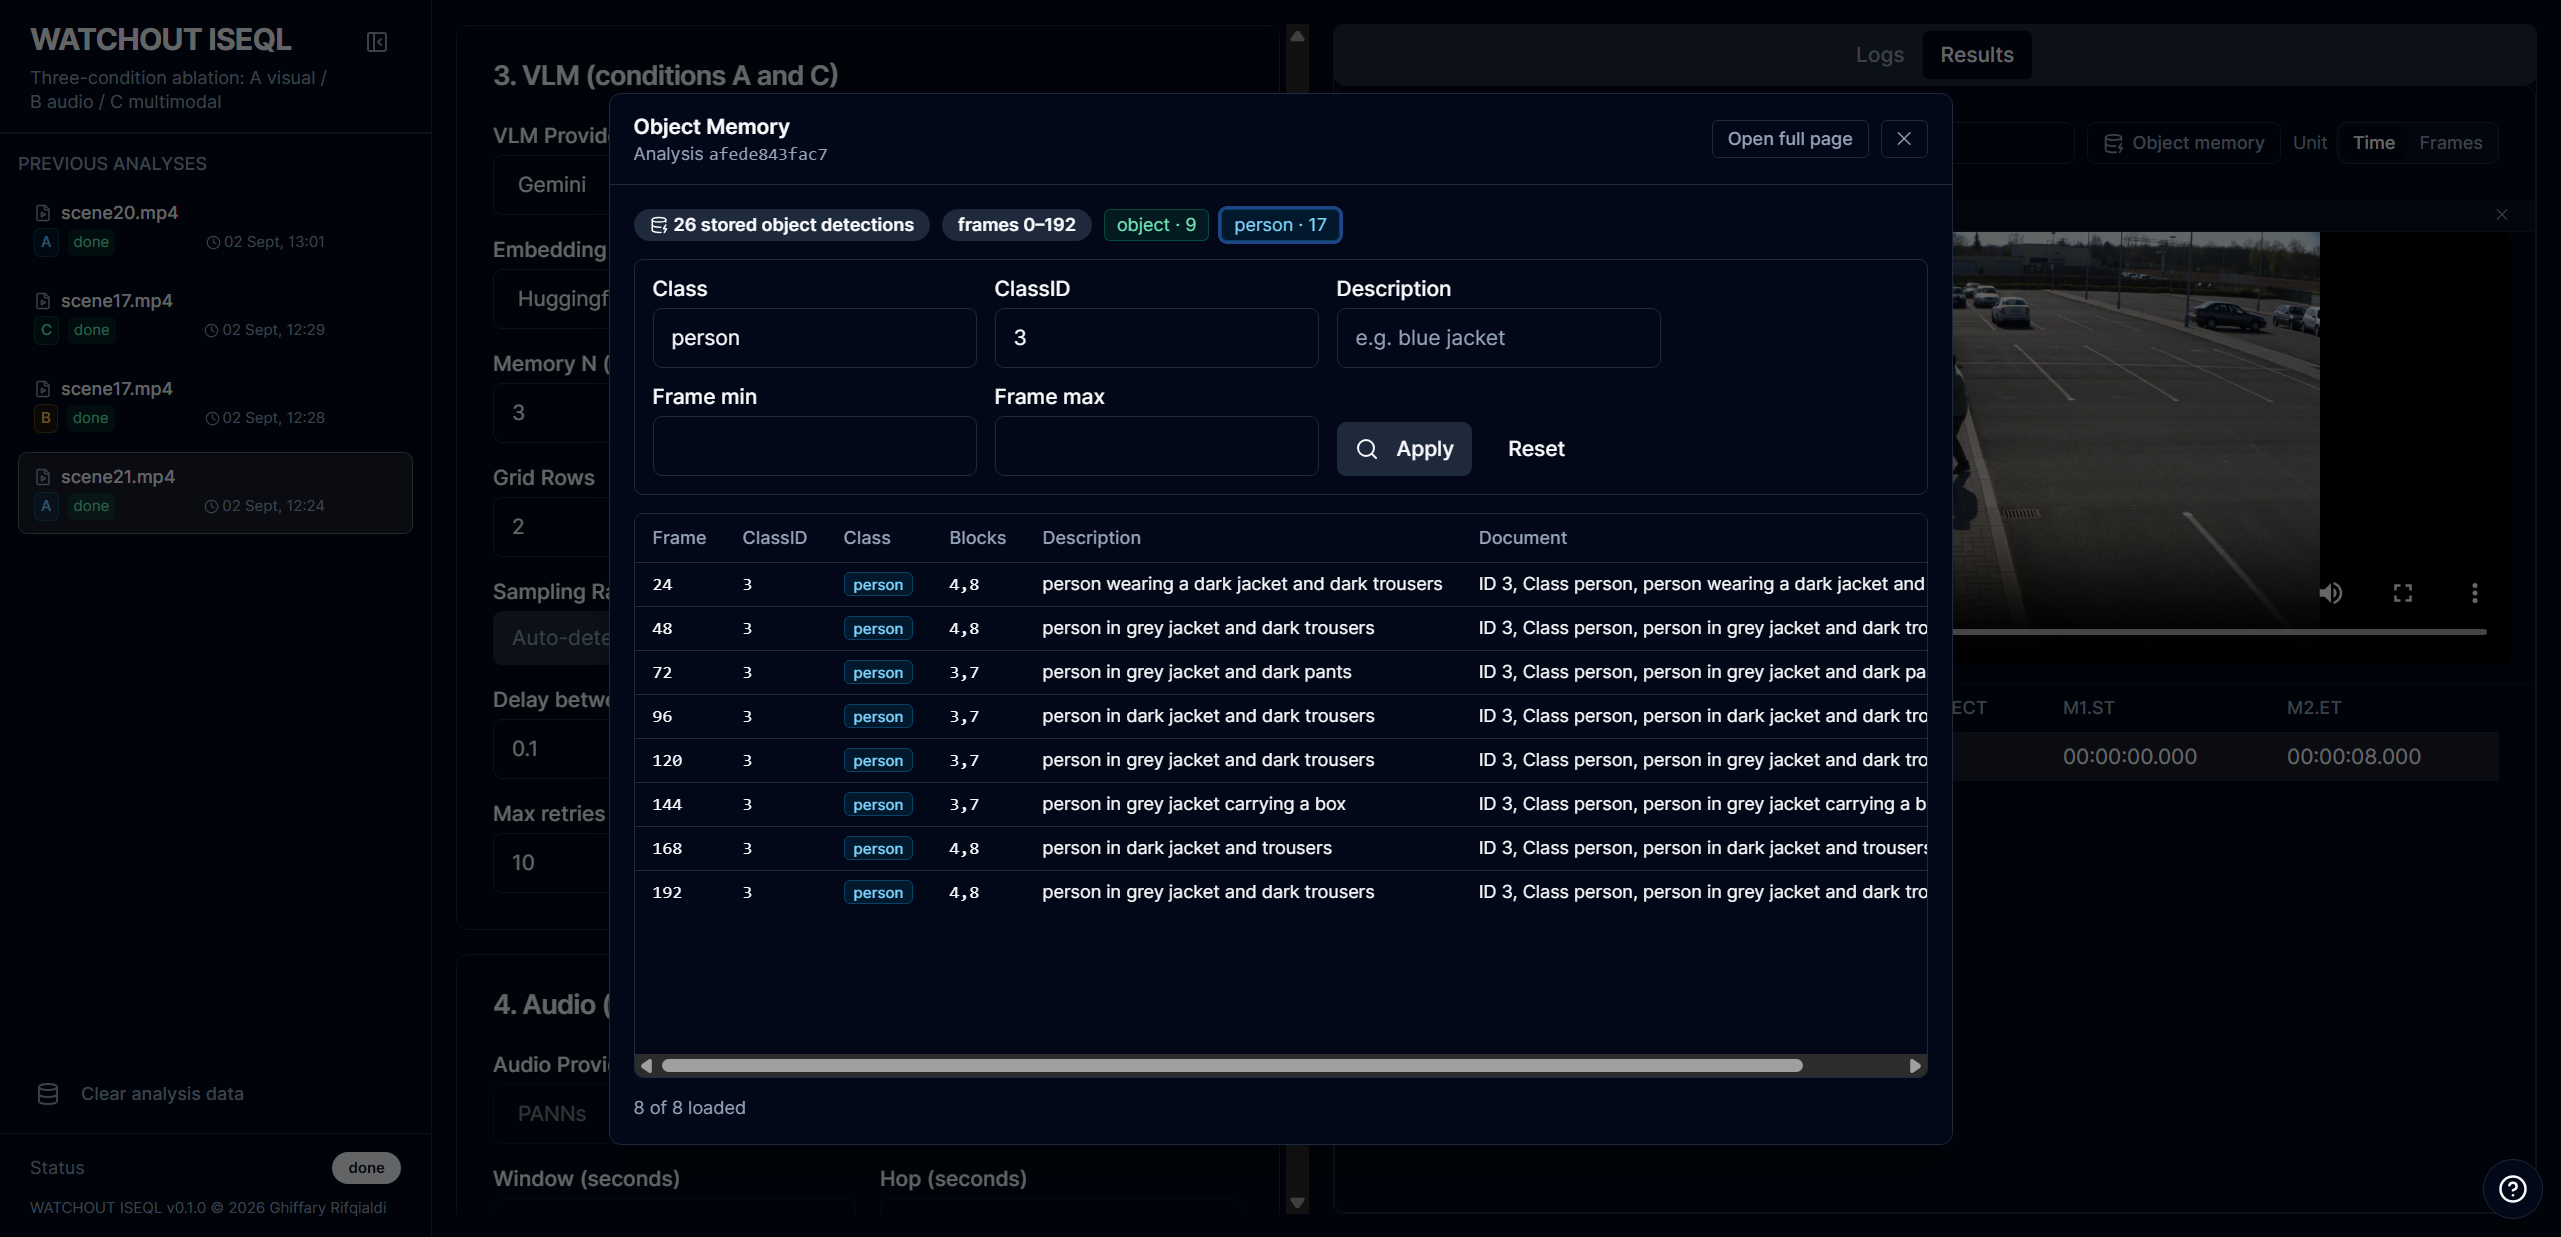
\includegraphics[width=0.92\textwidth]{Figures/appendix/va03_memory_person3.png}
  \caption{Object Memory (visual only, handoff example): person identity 3 (grey jacket); together with identity 1 this shows the handoff passed between two different people.}
\end{figure}

\begin{figure}[H]
  \centering
  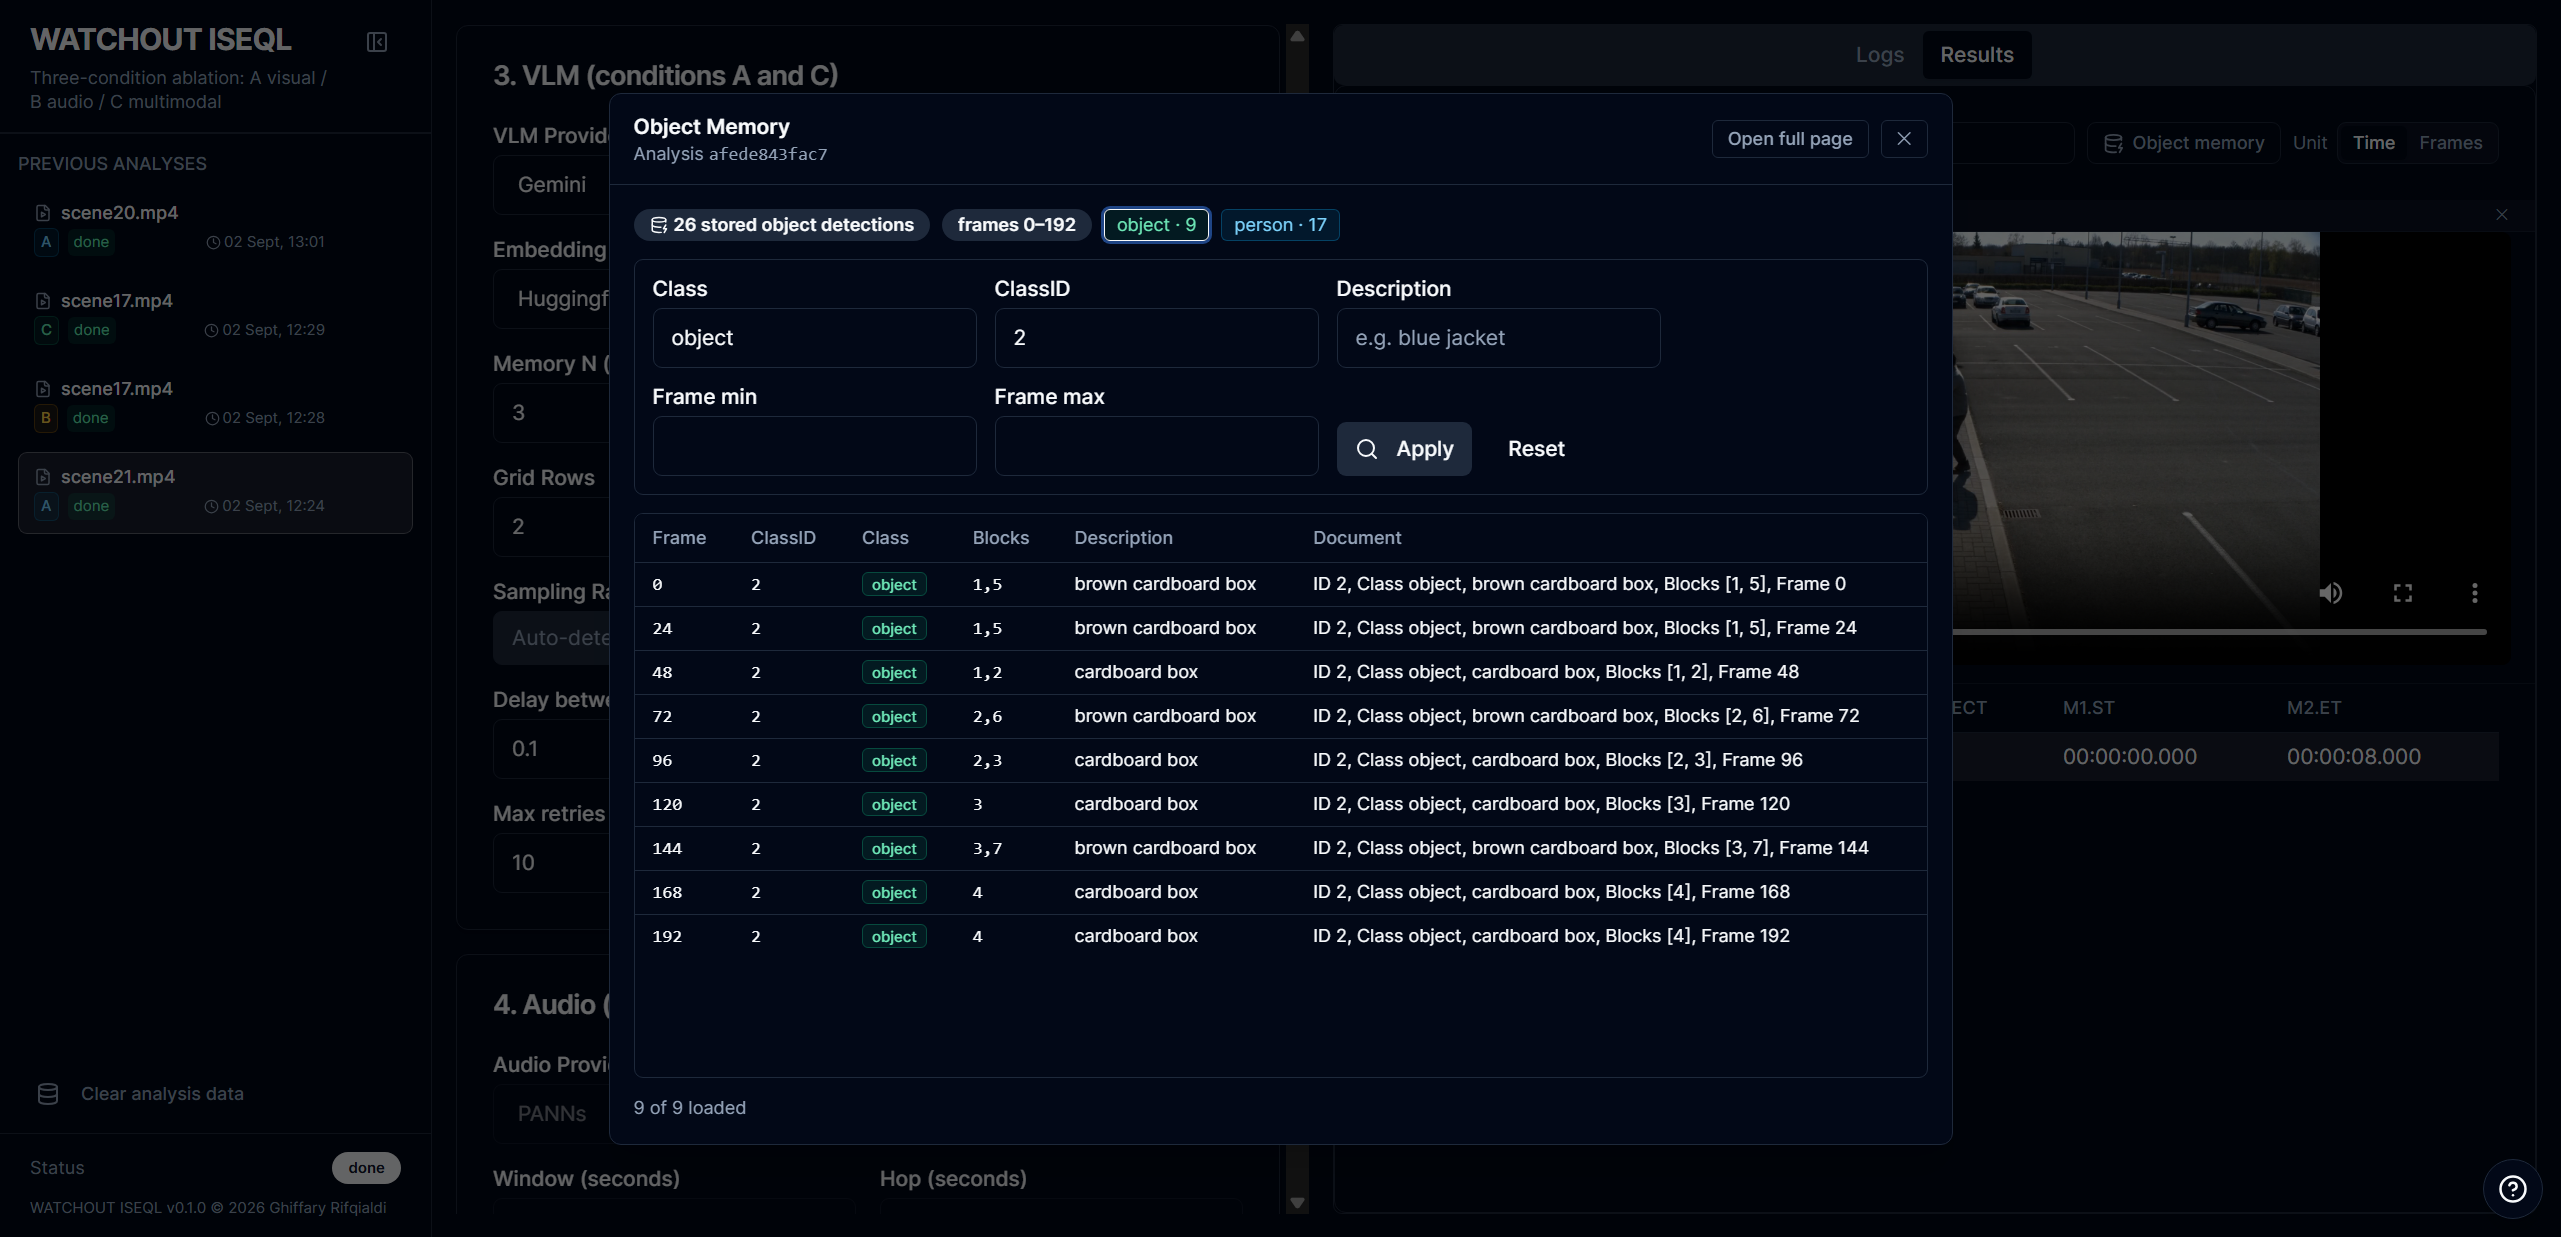
\includegraphics[width=0.92\textwidth]{Figures/appendix/va04_memory_object.png}
  \caption{Object Memory (visual only, handoff example): object identity 2 (brown cardboard box), the carried item referenced by the M1.OBJECT column, which changed hands between the two persons.}
\end{figure}

\section{Audio Only: Vehicle Collision}

This example runs condition B (audio only) through the Qwen2-Audio-7B LALM to detect the vehicle collision event from its audio signature.

\begin{figure}[H]
  \centering
  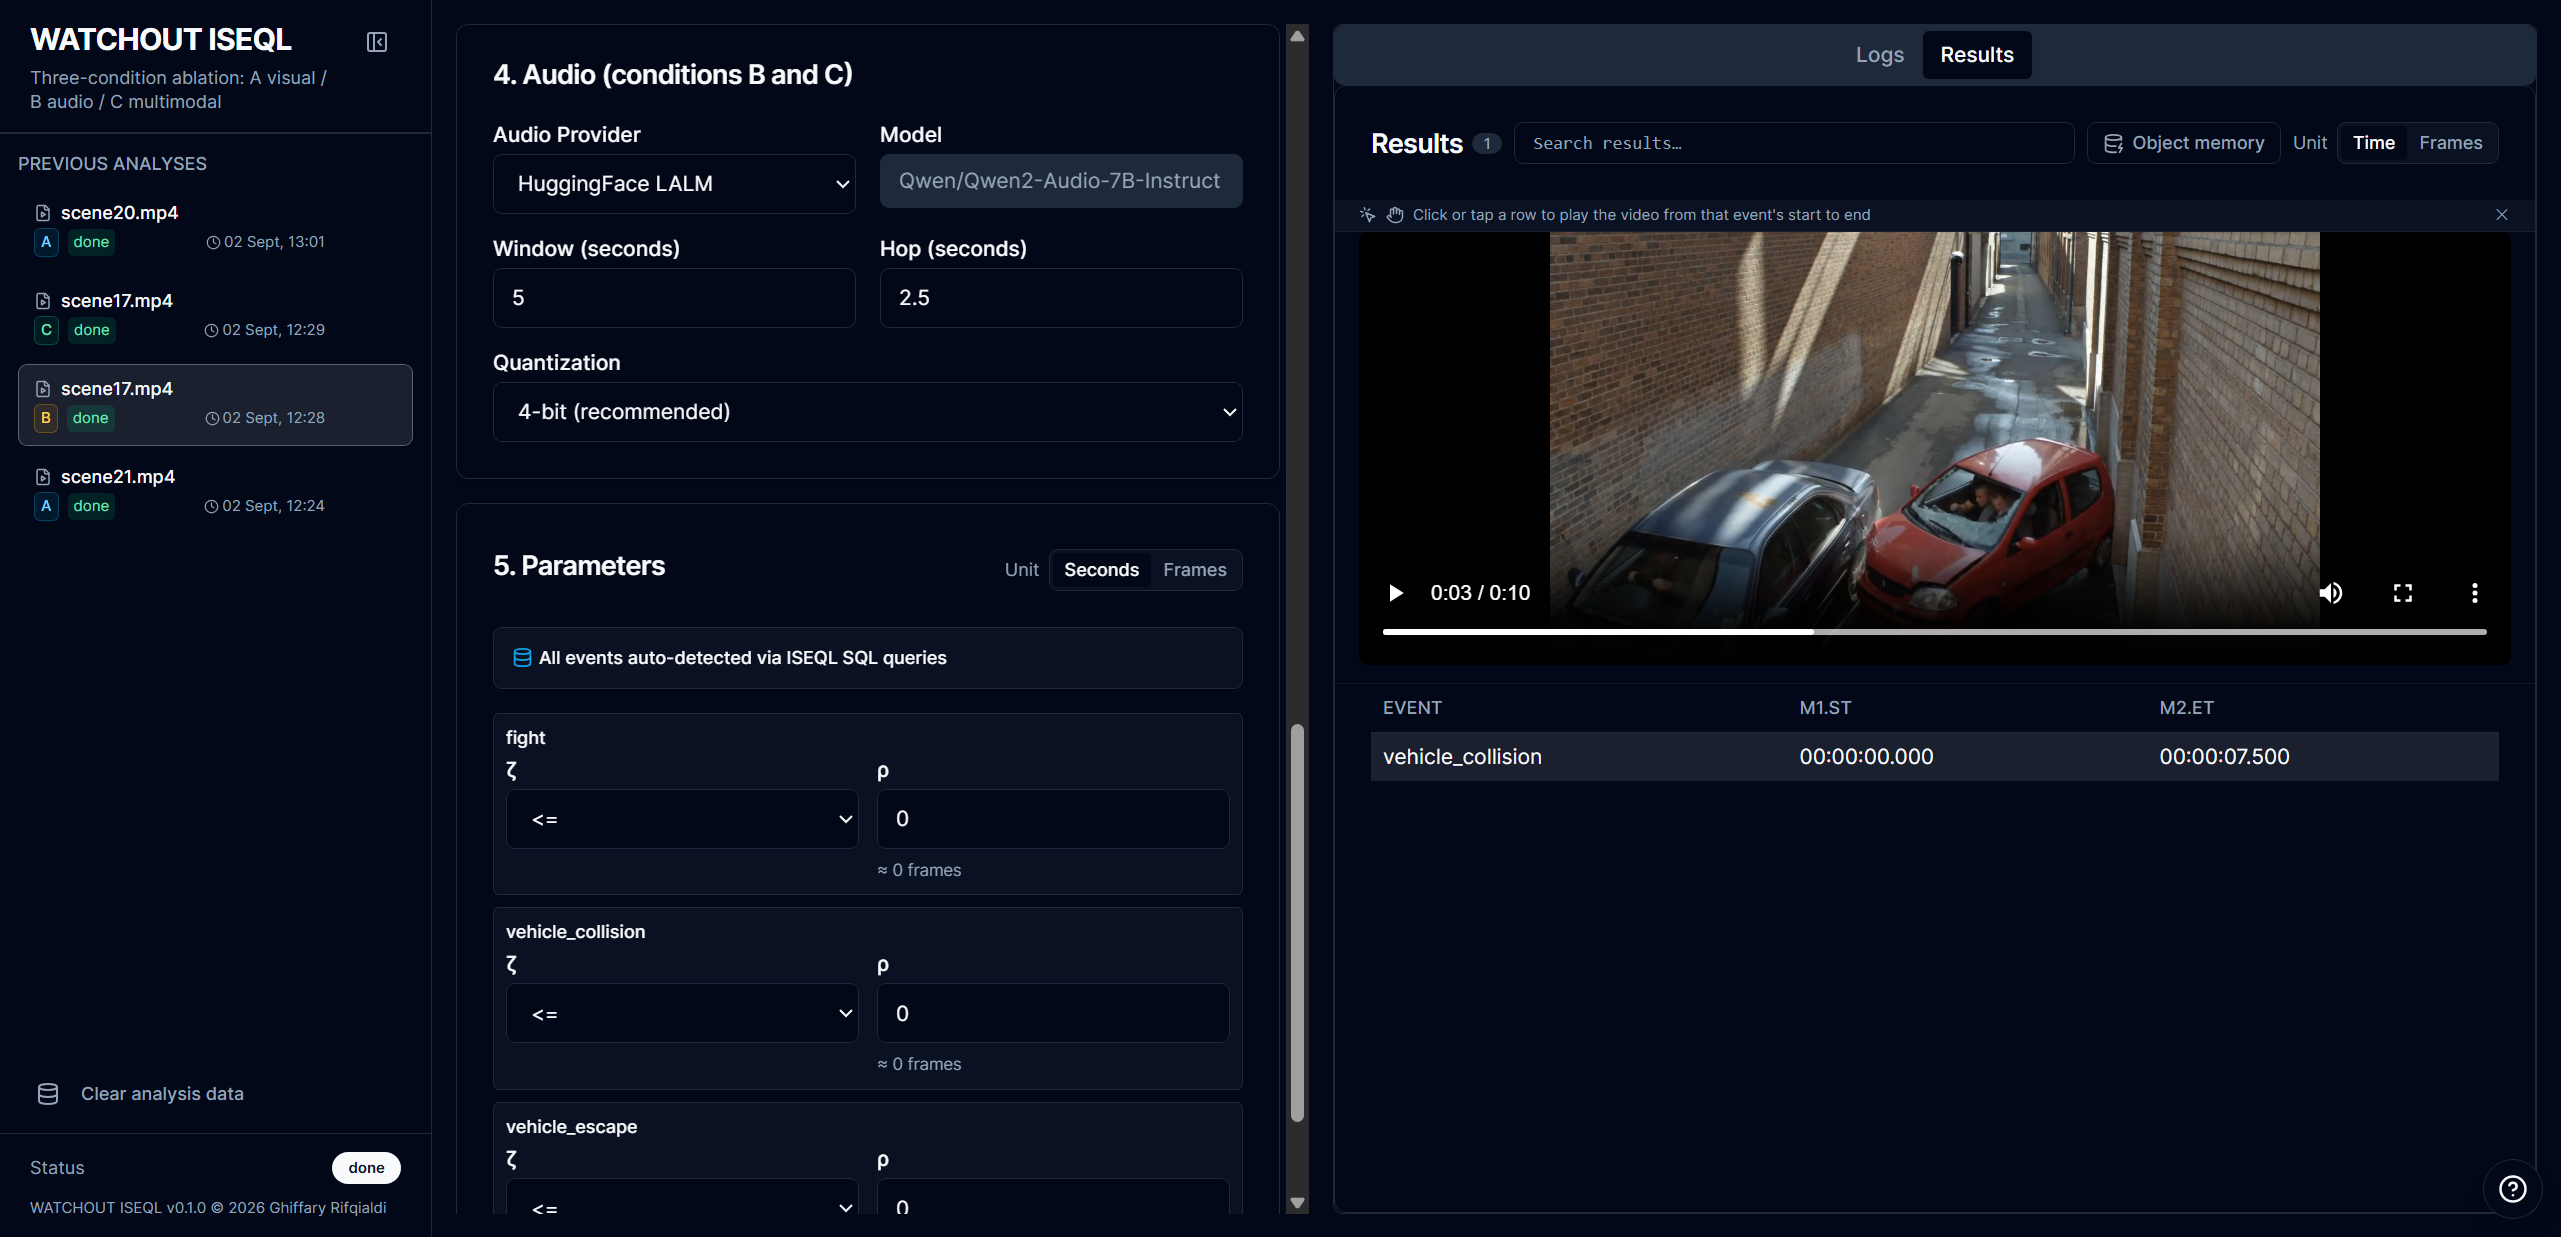
\includegraphics[width=0.92\textwidth]{Figures/appendix/ab01_results.png}
  \caption{Audio only (vehicle collision): the results report the vehicle collision detected from audio, with its start and end timestamps.}
\end{figure}

\section{Multimodal: Vehicle Collision}

This example runs condition C (multimodal), which combines the Gemini 3.6 Flash visual detection and the Qwen2-Audio-7B audio detection via set union, to detect the vehicle collision event using both modalities.

\begin{figure}[H]
  \centering
  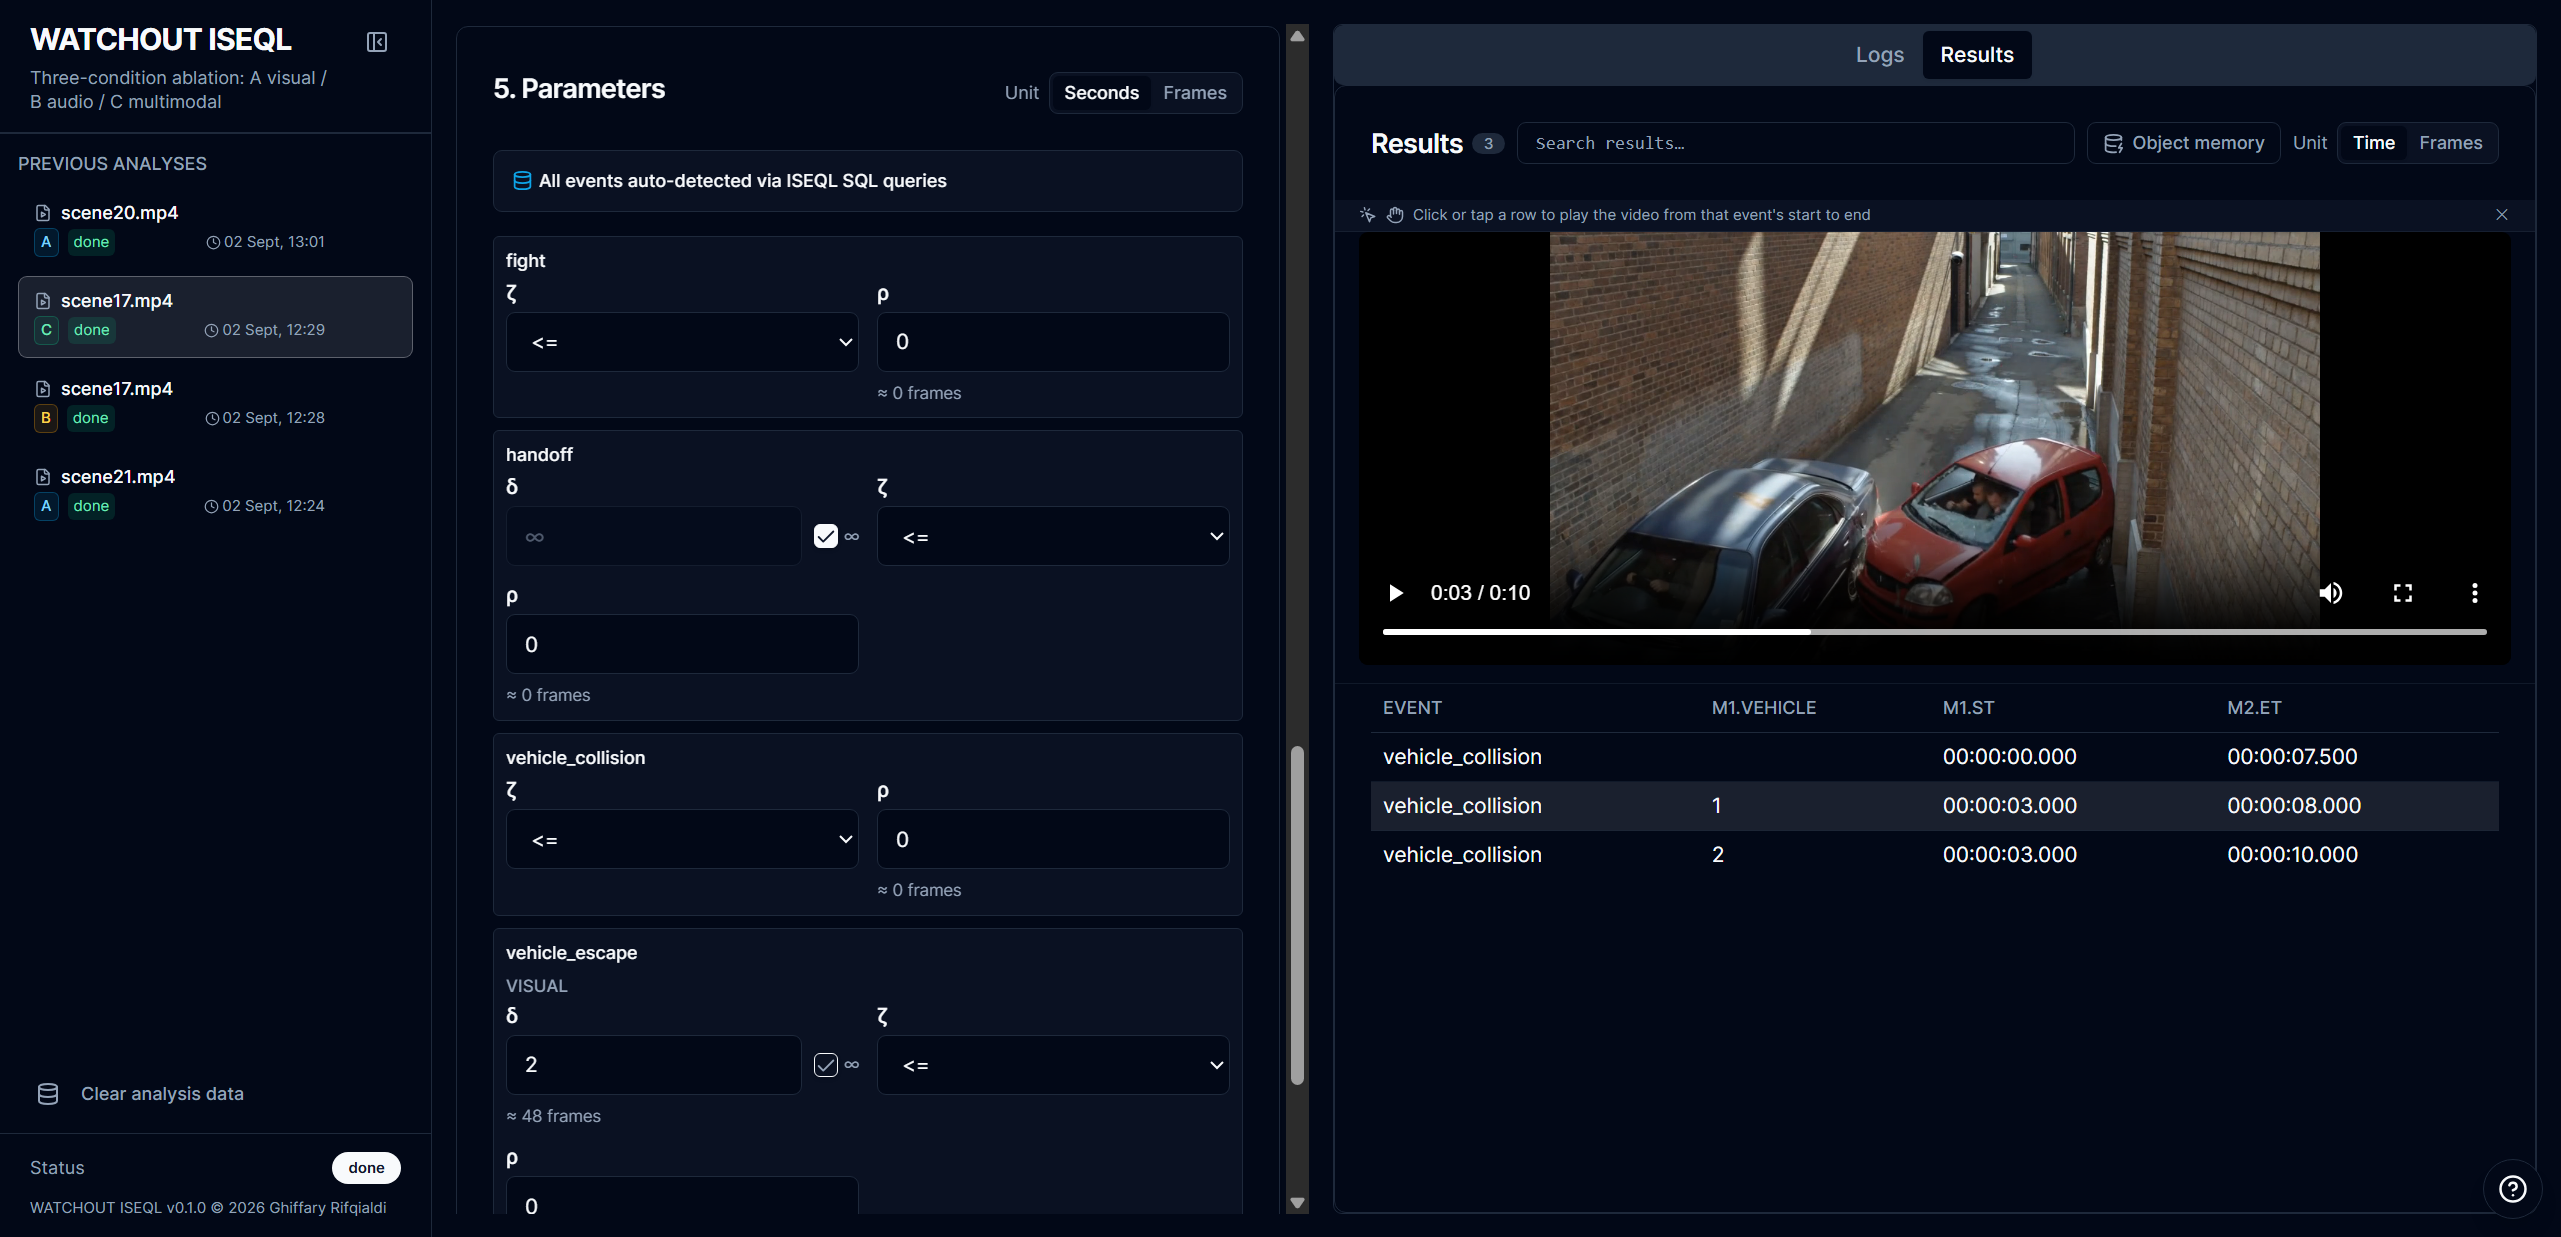
\includegraphics[width=0.92\textwidth]{Figures/appendix/mc01_results.png}
  \caption{Multimodal (vehicle collision): the results list the detected collisions with the M1.VEHICLE identity, so the specific vehicle involved can be identified across frames.}
\end{figure}

\begin{figure}[H]
  \centering
  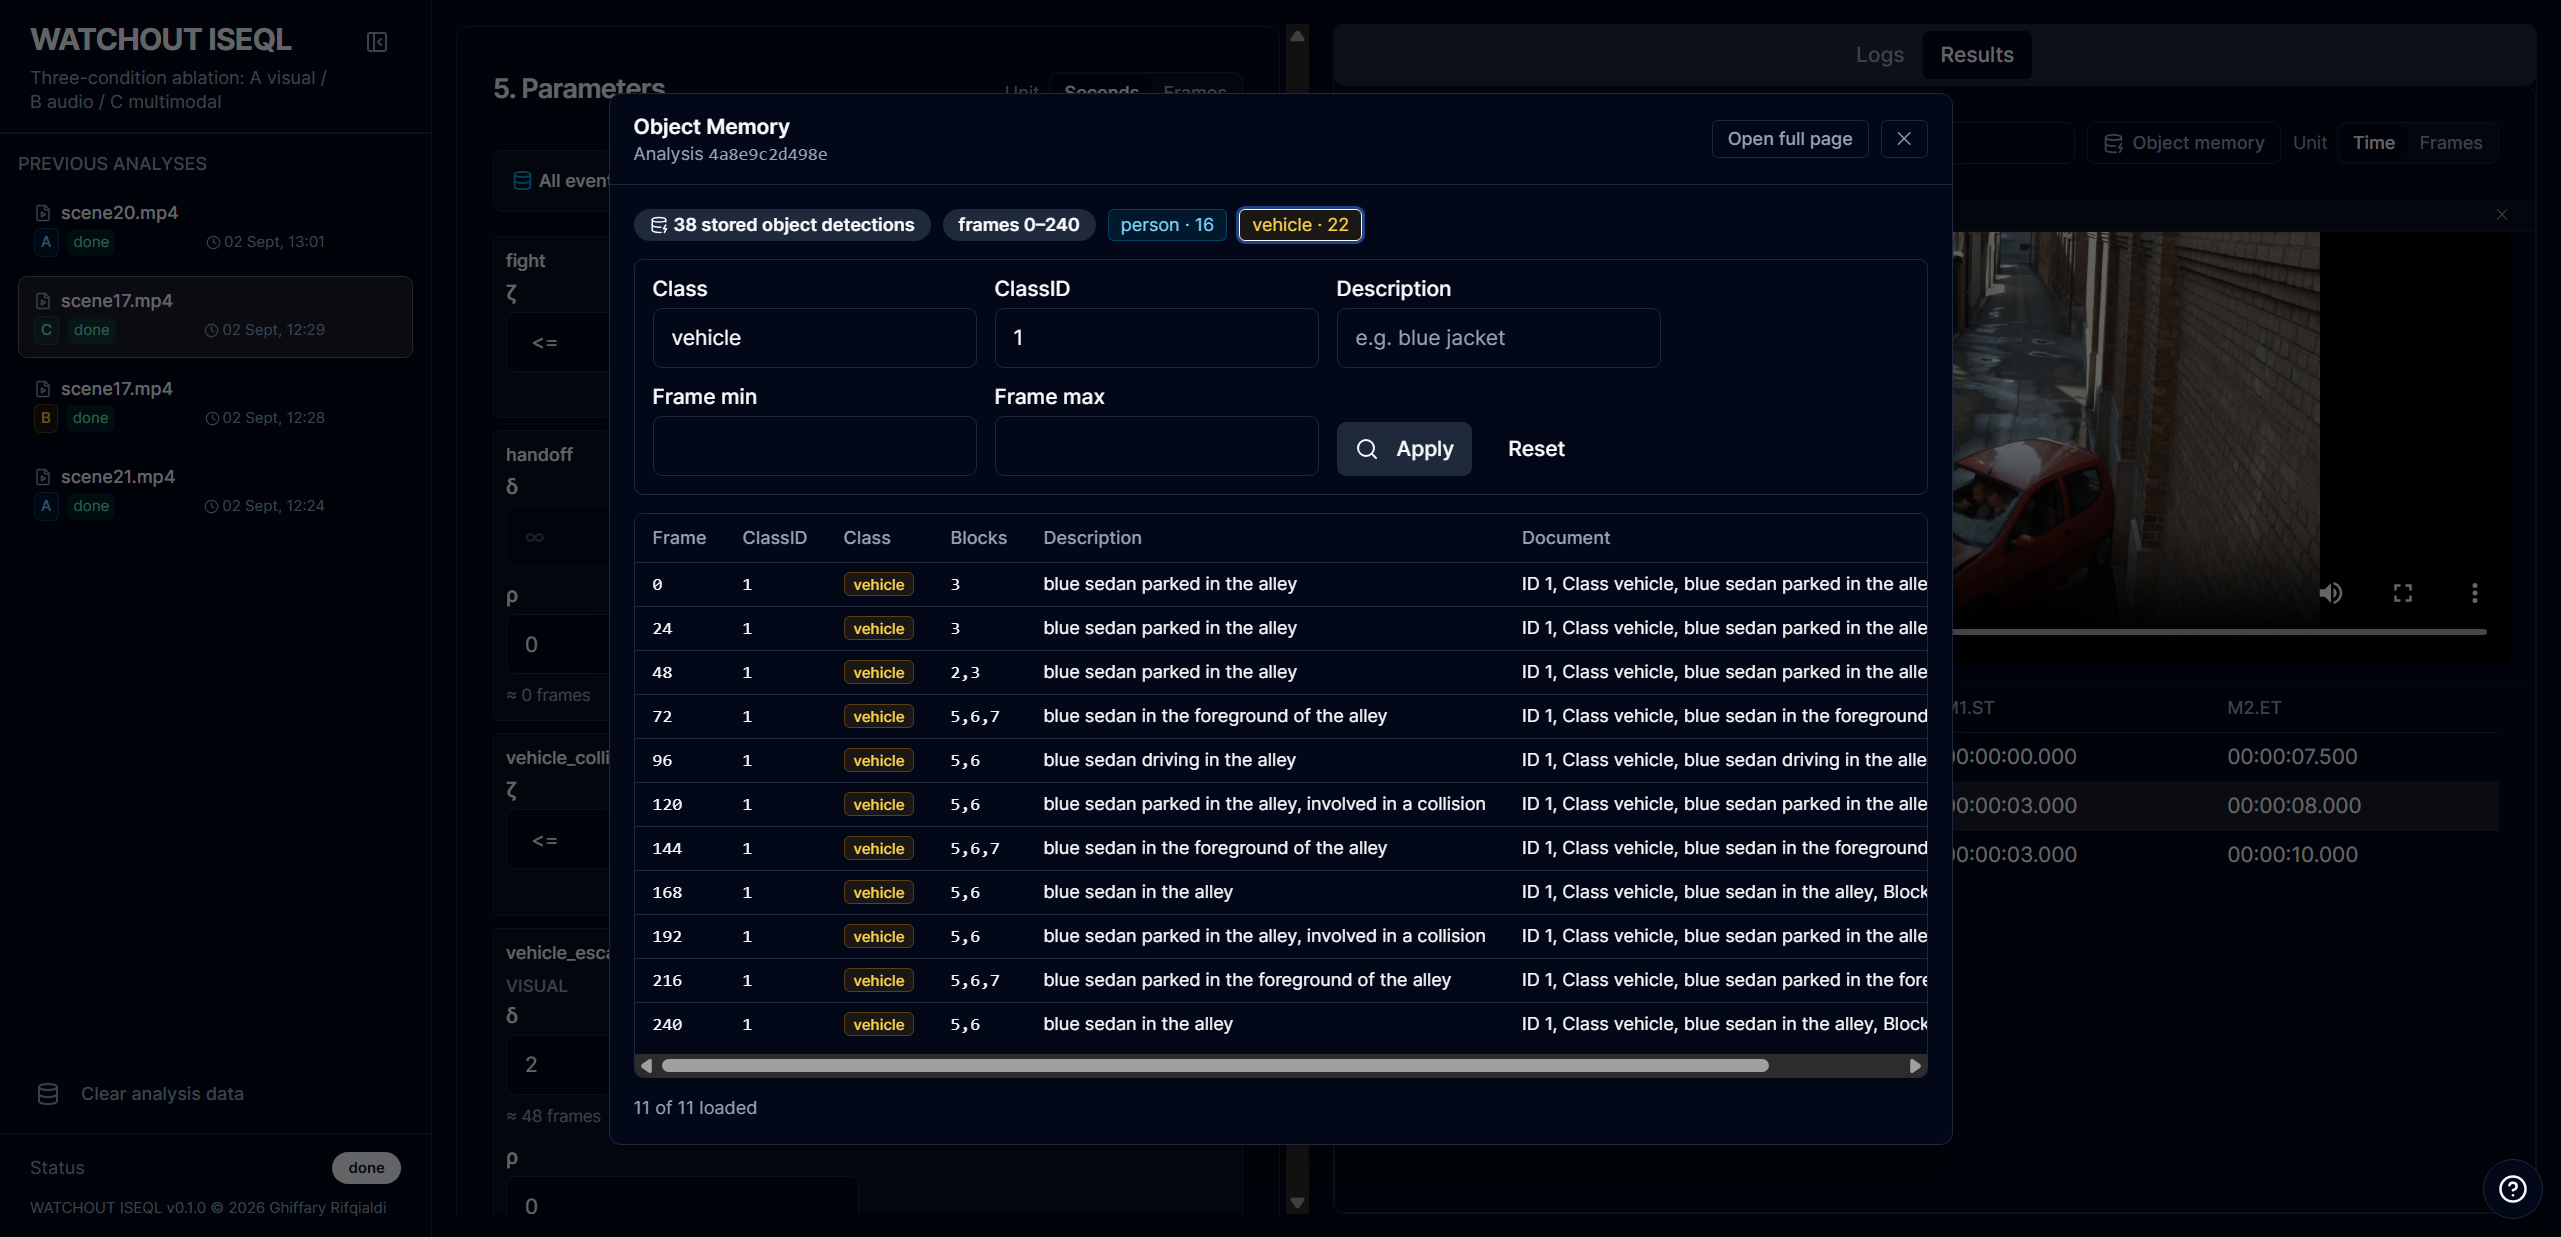
\includegraphics[width=0.92\textwidth]{Figures/appendix/mc02_memory_vehicle1.png}
  \caption{Object Memory (multimodal, vehicle collision example): vehicle identity 1 (red car); the M1.VEHICLE column in the result points to this vehicle.}
\end{figure}

\begin{figure}[H]
  \centering
  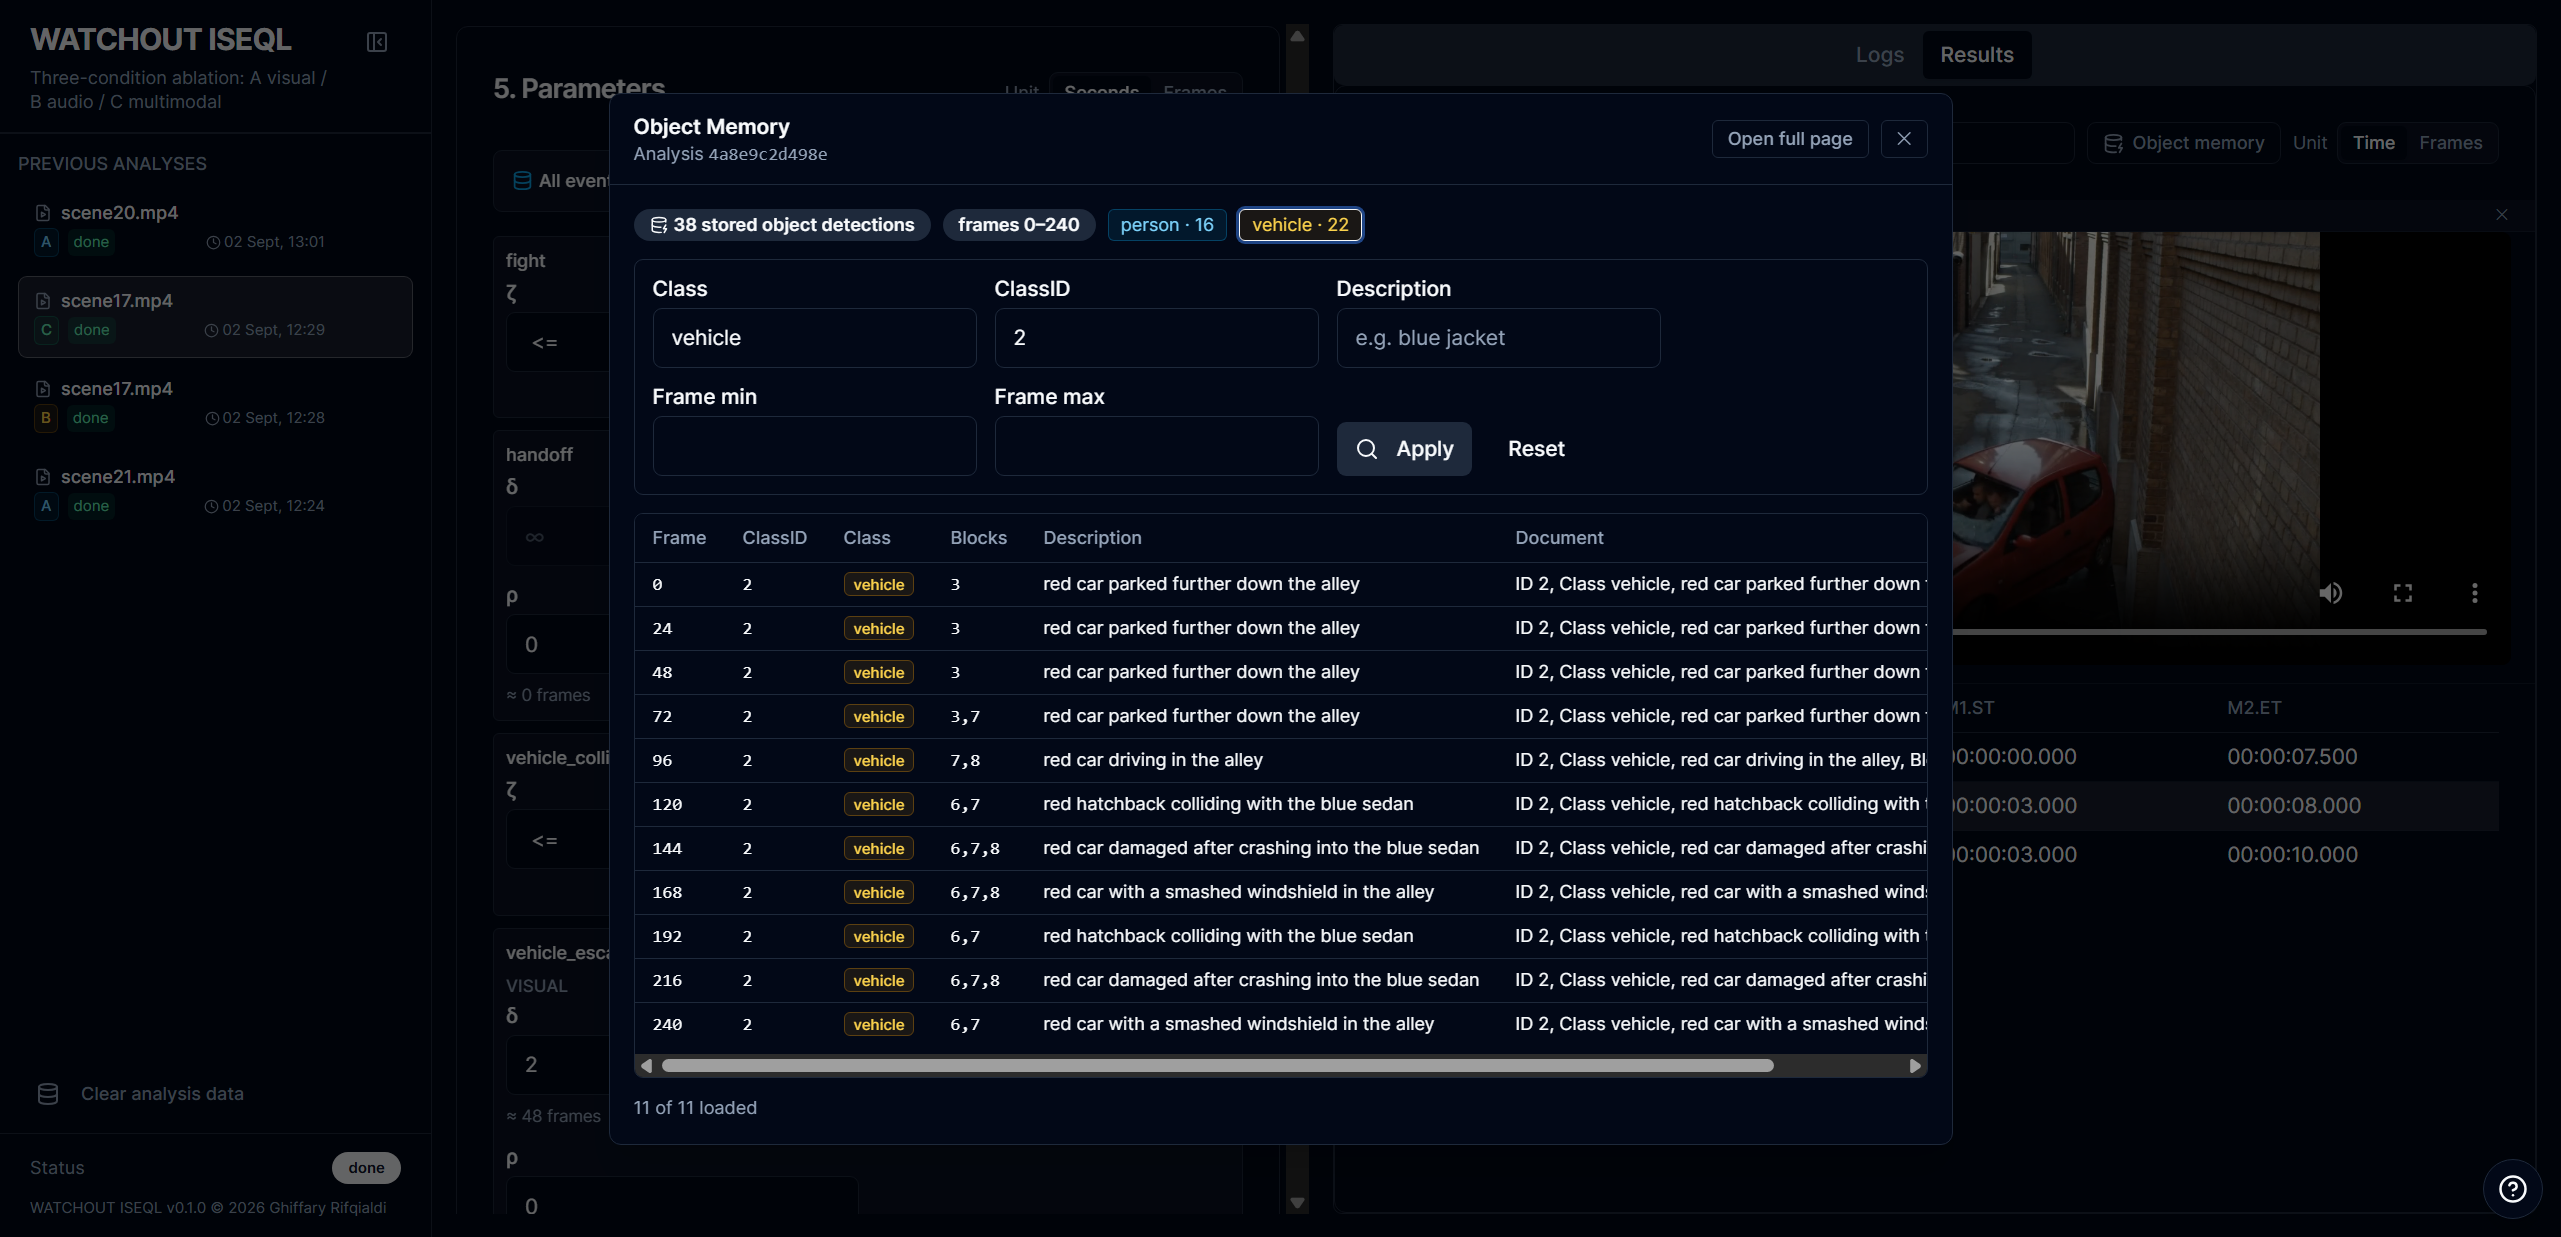
\includegraphics[width=0.92\textwidth]{Figures/appendix/mc03_memory_vehicle2.png}
  \caption{Object Memory (multimodal, vehicle collision example): vehicle identity 2 (a second car); the multimodal union reports both identities as separate detections.}
\end{figure}

%\include{Appendices/AppendixC}

%----------------------------------------------------------------------------------------
%  BIBLIOGRAPHY
%----------------------------------------------------------------------------------------

\printbibliography[heading=bibintoc]

%----------------------------------------------------------------------------------------

\end{document}
